\documentclass[handout]{beamer}\usepackage[]{graphicx}\usepackage[]{color}
%% maxwidth is the original width if it is less than linewidth
%% otherwise use linewidth (to make sure the graphics do not exceed the margin)
\makeatletter
\def\maxwidth{ %
  \ifdim\Gin@nat@width>\linewidth
    \linewidth
  \else
    \Gin@nat@width
  \fi
}
\makeatother

\definecolor{fgcolor}{rgb}{0.345, 0.345, 0.345}
\newcommand{\hlnum}[1]{\textcolor[rgb]{0.686,0.059,0.569}{#1}}%
\newcommand{\hlstr}[1]{\textcolor[rgb]{0.192,0.494,0.8}{#1}}%
\newcommand{\hlcom}[1]{\textcolor[rgb]{0.678,0.584,0.686}{\textit{#1}}}%
\newcommand{\hlopt}[1]{\textcolor[rgb]{0,0,0}{#1}}%
\newcommand{\hlstd}[1]{\textcolor[rgb]{0.345,0.345,0.345}{#1}}%
\newcommand{\hlkwa}[1]{\textcolor[rgb]{0.161,0.373,0.58}{\textbf{#1}}}%
\newcommand{\hlkwb}[1]{\textcolor[rgb]{0.69,0.353,0.396}{#1}}%
\newcommand{\hlkwc}[1]{\textcolor[rgb]{0.333,0.667,0.333}{#1}}%
\newcommand{\hlkwd}[1]{\textcolor[rgb]{0.737,0.353,0.396}{\textbf{#1}}}%
\let\hlipl\hlkwb

\usepackage{framed}
\makeatletter
\newenvironment{kframe}{%
 \def\at@end@of@kframe{}%
 \ifinner\ifhmode%
  \def\at@end@of@kframe{\end{minipage}}%
  \begin{minipage}{\columnwidth}%
 \fi\fi%
 \def\FrameCommand##1{\hskip\@totalleftmargin \hskip-\fboxsep
 \colorbox{shadecolor}{##1}\hskip-\fboxsep
     % There is no \\@totalrightmargin, so:
     \hskip-\linewidth \hskip-\@totalleftmargin \hskip\columnwidth}%
 \MakeFramed {\advance\hsize-\width
   \@totalleftmargin\z@ \linewidth\hsize
   \@setminipage}}%
 {\par\unskip\endMakeFramed%
 \at@end@of@kframe}
\makeatother

\definecolor{shadecolor}{rgb}{.97, .97, .97}
\definecolor{messagecolor}{rgb}{0, 0, 0}
\definecolor{warningcolor}{rgb}{1, 0, 1}
\definecolor{errorcolor}{rgb}{1, 0, 0}
\newenvironment{knitrout}{}{} % an empty environment to be redefined in TeX

\usepackage{alltt}

\usepackage{default}
\usepackage{animate} %need the animate.sty file 
\usepackage{graphicx}
%\graphicspath{{/home/sahir/Dropbox/jobs/laval/minicours/slides/}}
\usepackage{hyperref, url}
%\usepackage[round,sort]{natbib}   % bibliography omit 'round' option if you prefer square brackets
%\bibliographystyle{apalike}
\usepackage{biblatex}
\bibliography{bib.bib}
% Removes icon in bibliography
\setbeamertemplate{bibliography item}[text]

\usepackage[normalem]{ulem}

\setbeamertemplate{theorems}[numbered]



%\newtheorem{prop}{Proposition}
%\newenvironment{theoremc}[1]
%{\begin{shaded}\begin{theorem}[#1]}
%		{\end{theorem}\end{shaded}}
	
%\newtheorem{examplefirst}{Example}
%\newtheorem{examplesecond}{Example}
%\newenvironment<>{examplefirst}[1][]{%
%	\setbeamercolor{block title example}{bg=lightgray}%
%	\begin{example}#2[#1]}{\end{example}}
%\newenvironment<>{examplesecond}[1][]{%
%	\setbeamercolor{block title example}{fg=white,bg=blue!75!black}%
%	\begin{example}#2[#1]}{\end{example}}	

%\usepackage{amsthm}


\usepackage[figurename=Fig.]{caption}
\usepackage{subfig}
\usepackage{tikz, pgfplots,epsfig}
\usetikzlibrary{arrows,shapes.geometric}
\usepackage{color, colortbl,xcolor}
\definecolor{lightgray}{RGB}{200,200,200}
\definecolor{palegray}{RGB}{221,221,221}
\definecolor{myblue}{RGB}{0,89,179}
\usepackage{comment}
\setbeamercolor{frametitle}{fg=myblue}
\setbeamercolor{section in head/foot}{bg=myblue, fg=white}
\setbeamercolor{author in head/foot}{bg=myblue}
\setbeamercolor{date in head/foot}{bg=myblue}

\usepackage{shadethm}
%\colorlet{shadecolor}{blue!15}
\colorlet{shadecolor}{palegray}
%\setlength{\shadeboxrule}{.4pt}

\newshadetheorem{thm}{Theorem}
\newshadetheorem{defm}{Definition}
\newshadetheorem{exm}{Exercise}
\newshadetheorem{remarkm}{Remark}
%\definecolor{shadethmcolor}{HTML}{EDF8FF}
\definecolor{shadethmcolor}{RGB}{221,221,221}
%\definecolor{shaderulecolor}{HTML}{45CFFF}
\definecolor{shaderulecolor}{RGB}{0,89,179}
\setlength{\shadeboxrule}{.4pt}


\usepackage{array}
\newcolumntype{L}{>{\centering\arraybackslash}m{3cm}} % used for text wrapping in ctable
\usepackage{ctable}
\usepackage[utf8]{inputenc}
\usepackage{fontenc}
\usepackage{pifont}% http://ctan.org/pkg/pifont
\newcommand{\cmark}{\ding{51}}%
\newcommand{\xmark}{\ding{55}}%
\def\widebar#1{\overline{#1}}
\definecolor{whitesmoke}{rgb}{0.96, 0.96, 0.96}

\usepackage{amssymb}
\usepackage{amsmath}

\usepackage{bm}
\def\transpose{{\sf{T}}}
\def\E{{\skew0\bm{E}}}
\def\Xvec{{\skew0\bm{X}}}
\def\Xveca{{\skew0\bm{X}}_1}
\def\Xvecb{{\skew0\bm{X}}_2}

\def\Yvec{{\skew0\bm{Y}}}
\def\bmY{{\skew0\bm{Y}}}
\def\bmX{{\skew0\bm{X}}}
\def\bmy{{\skew0\bm{y}}}
\def\bmG{{\skew0\bm{G}}}
\def\bmS{{\skew0\bm{S}}}
\def\bmA{{\skew0\bm{A}}}
\def\bmB{{\skew0\bm{B}}}
\def\bmD{{\skew0\bm{D}}}
\def\bmI{{\skew0\bm{I}}}
\def\bmV{{\skew0\bm{V}}}
\def\bmU{{\skew0\bm{U}}}
\def\bv{{\skew0\bm{v}}}
\def\bw{{\skew0\bm{w}}}
\def\bmm{{\skew0\bm{m}}}
\def\bmzero{{\skew0\bm{0}}}
\def\bx{{\skew0\bm{x}}}
\def\xveca{{\skew0\bm{x}}_1}
\def\xvecb{{\skew0\bm{x}}_2}

\def\N{{\skew0\mathcal{N}}}
\def\T{{\small T}}

\def\mvec{{\skew0\bm{m}}}
\def\bmmu{{\skew0\bm{\mu}}}
\def\muvec{{\skew0\bm{\mu}}}
\def\balpha{{\skew0\bm{\alpha}}}
\def\bbeta{{\skew0\bm{\beta}}}
\def\bmtheta{{\skew0\bm{\theta}}}
\def\btheta{{\skew0\bm{\theta}}}

\def\cvec{{\skew0\mathbf{c}}}

\def\Xbar{\overline{X}}

\definecolor{lightgray}{rgb}{0.91,0.91,0.91}
\definecolor{purpleblue}{rgb}{0.50,0.50,1.00}



\usepackage{fontspec}
%\setsansfont{Fira Sans}
%\setmonofont{Fira Mono}
\setsansfont[ItalicFont={Fira Sans Light Italic},BoldFont={Fira Sans},BoldItalicFont={Fira Sans Italic}]{Fira Sans Light}
\setmonofont[BoldFont={Fira Mono Medium}]{Fira Mono}


\setbeamercolor{itemize item}{fg=myblue}
\setbeamertemplate{itemize item}[square]

\setbeamertemplate{navigation symbols}{\usebeamercolor[fg]{title in head/foot}\usebeamerfont{title in head/foot}\insertframenumber}
\setbeamertemplate{footline}{}

\newtheorem{proposition}[theorem]{Proposition}
\newtheorem{exercise}[theorem]{Exercise}

\titlegraphic{\hfill
\includegraphics[height=1cm]{mcgill_logo.png}}


%% You also use hyperref, and pick colors 
\hypersetup{colorlinks,citecolor=orange,filecolor=red,linkcolor=brown,urlcolor=blue}

\newcommand {\framedgraphiccaption}[2] {
	\begin{figure}
		\centering
		\includegraphics[width=\textwidth,height=0.8\textheight,keepaspectratio]{#1}
		\caption{#2}
	\end{figure}
}

\newcommand {\framedgraphic}[1] {
	\begin{figure}
		\centering
		\includegraphics[width=\textwidth,height=0.9\textheight,keepaspectratio]{#1}
	\end{figure}
}


\AtBeginSection[]{
	\begin{frame}
		\vfill
		\centering
		\begin{beamercolorbox}[sep=8pt,center,shadow=true,rounded=true]{title}
			\usebeamerfont{title}\insertsectionhead\par%
		\end{beamercolorbox}
		\vfill
	\end{frame}
}

\newcommand\Wider[2][3em]{%
	\makebox[\linewidth][c]{%
		\begin{minipage}{\dimexpr\textwidth+#1\relax}
			\raggedright#2
		\end{minipage}%
	}%
}



\newcommand{\blue}[1]{\textcolor{blue}{#1}}
\newcommand{\red}[1]{\textcolor{red}{#1}}
%\makeatother

\usepackage{xparse}
\NewDocumentCommand\mylist{>{\SplitList{;}}m}
{
	\begin{itemize}
		\ProcessList{#1}{ \insertitem }
	\end{itemize}
}
\NewDocumentCommand\mynum{>{\SplitList{;}}m}
{
	\begin{enumerate}
		\ProcessList{#1}{ \insertitem }
	\end{enumerate}
}
\newcommand\insertitem[1]{\item #1}

\newcommand\FrameText[1]{%
	\begin{textblock*}{\paperwidth}(0pt,\textheight)
		\raggedright #1\hspace{.5em}
\end{textblock*}}
\IfFileExists{upquote.sty}{\usepackage{upquote}}{}
\begin{document}
%\sffamily



%\title{Introduction to Regression Trees}
%\author{Sahir Bhatnagar \inst{1}}
%\author[shortname]{Sahir Rai Bhatnagar, PhD Candidate (Biostatistics) }
%\institute[shortinst]{Department of Epidemiology, Biostatistics and Occupational Health}

\title{$p$-values, Power and Sample Size}
\subtitle{JH Notes: Inference about a Population Mean ($\mu$)}
\author{Sahir Bhatnagar and James Hanley}
\institute{
	EPIB 607\\
	Department of Epidemiology, Biostatistics, and Occupational Health\\
	McGill University\\
	
	\vspace{0.1 in}
	
	\texttt{sahir.bhatnagar@mcgill.ca}\\
	\texttt{\url{https://sahirbhatnagar.com/EPIB607/}}}

%\date

\maketitle

\section{$p$-values}
\begin{frame}
\frametitle{$p$-values and statistical tests}


%\vspace{18pt}
\begin{defm}[$p$-value]
	A \textbf{probability concerning the observed data}, calculated under a \textbf{Null Hypothesis} assumption, i.e., assuming that the only factor operating is sampling or measurement variation. 
\end{defm}

\begin{itemize} 
	\item[\underline{Use}] To assess the evidence provided by the sample data
	in relation to a pre-specified claim or `hypothesis' concerning some parameter(s) or data-generating process. 
	\item[\underline{Basis}] As with a confidence interval, it makes use of the concept of a \textit{distribution}. 
	\item[\underline{Caution}] A $p$-value is NOT the probability that the null `hypothesis' is true
\end{itemize}
\end{frame}


\begin{frame}

\frametitle{Example 1 -- from \textit{Design of Experiments}, by R.A. Fisher}

\parindent 128pt
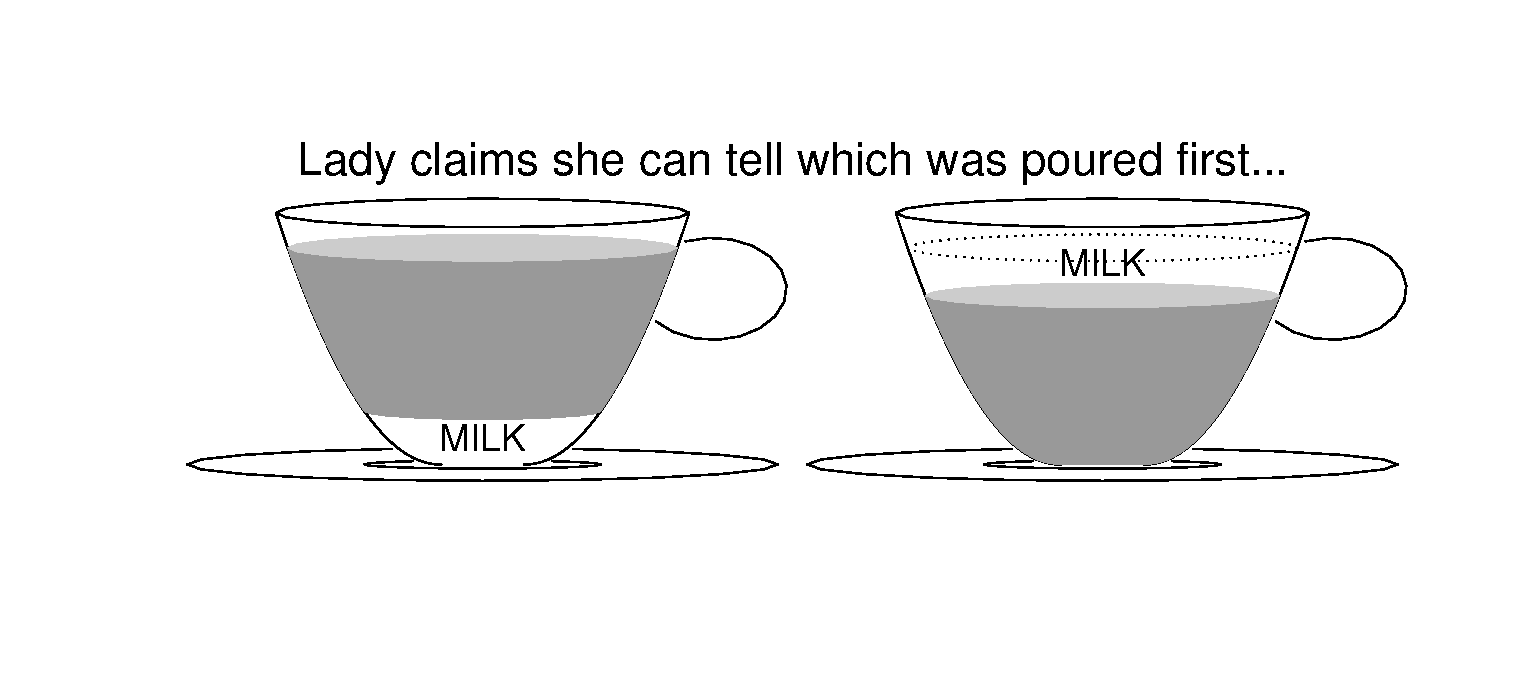
\includegraphics[width=1.8in]{TeaClaim.pdf}
\parindent 0pt

\begin{center}
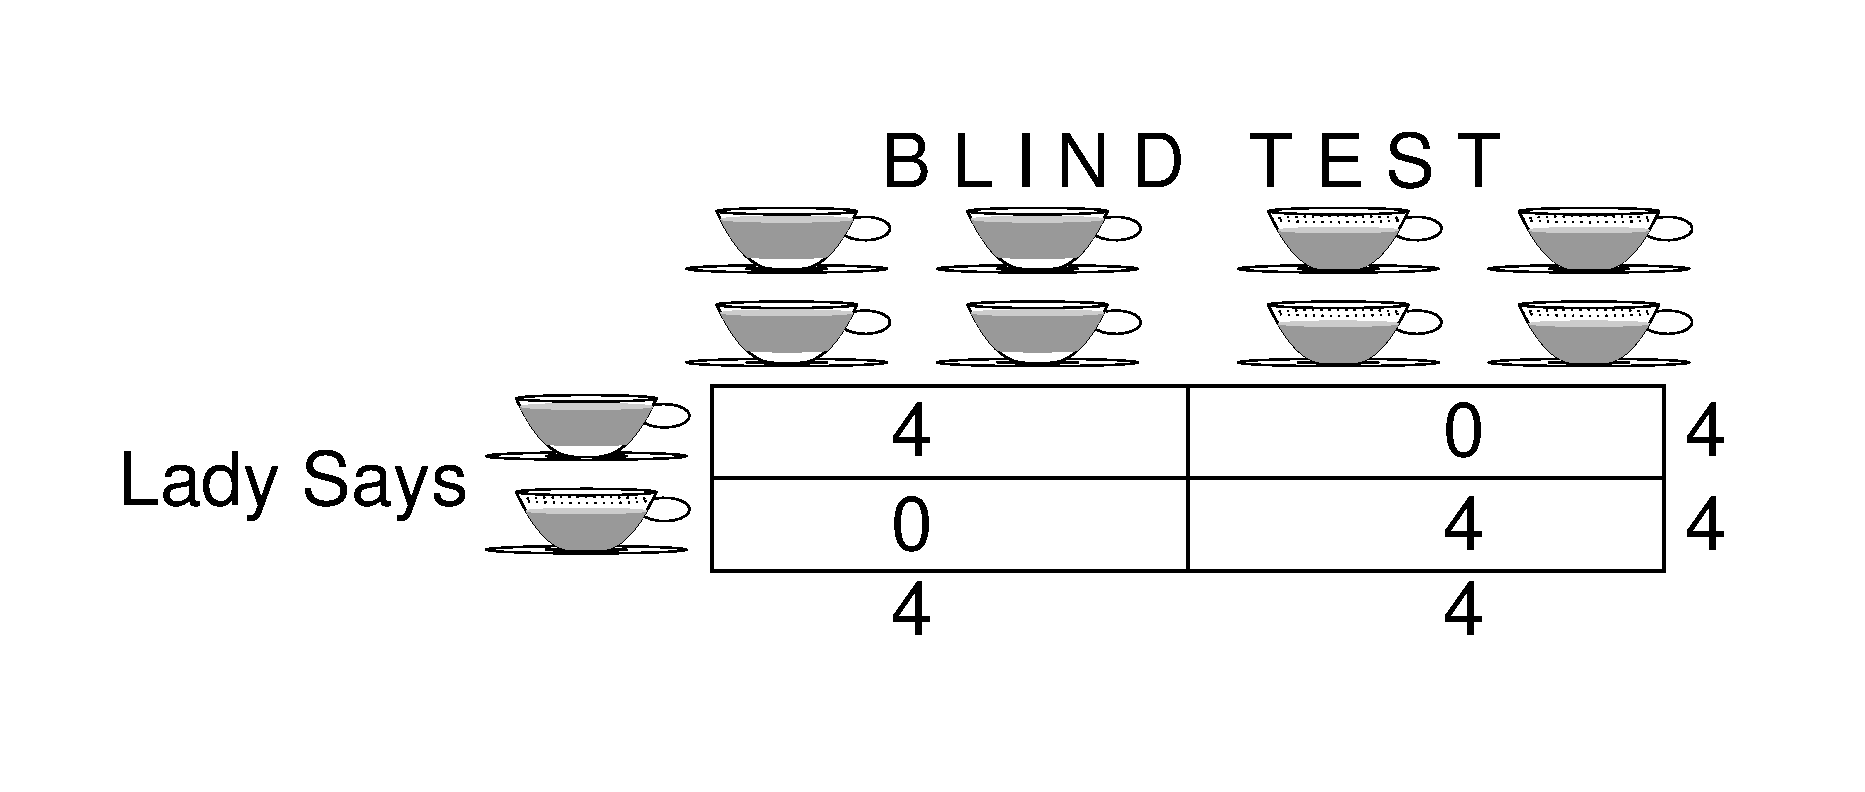
\includegraphics[width=3in]{BlindTest.pdf}
\end{center}
\blue{Null Hypothesis (H$_{null}$)}: she can not tell them apart, i.e., just guessing. \\ \ \\
\blue{Alternative Hypothesis (H$_{alt}$)}: she can. \\ \ \\ \pause

%\begin{scriptsize}
%	Blind test is equivalent to
%	being asked to say \textbf{which 4} of the following 8 Gaelic words  are the \textbf{correctly spelled}
%	ones. You are told that \textbf{4 are correctly spelled \& 4 are not}. 
%	\begin{center}
%		\begin{tabular}{c c c c  c c c c}
%			1&2&3&4&5&6&7&8\\
%			madra&olscoil&cathiar&tanga&doras&cluicha&f\'ear&b\'othar \\
%		\end{tabular}
%	\end{center} 
%\end{scriptsize}


\end{frame}

\begin{frame}
\frametitle{The evidence provided by the test}

\begin{footnotesize}
\begin{itemize}
\item
Rank possible test
results by  degree of evidence against H$_{null}$. 
\item ``$p$-value'' is the probability, calculated under null hypothesis, of
observing a result as  extreme as, or more extreme than, the one that was obtained/observed.
\begin{center}
	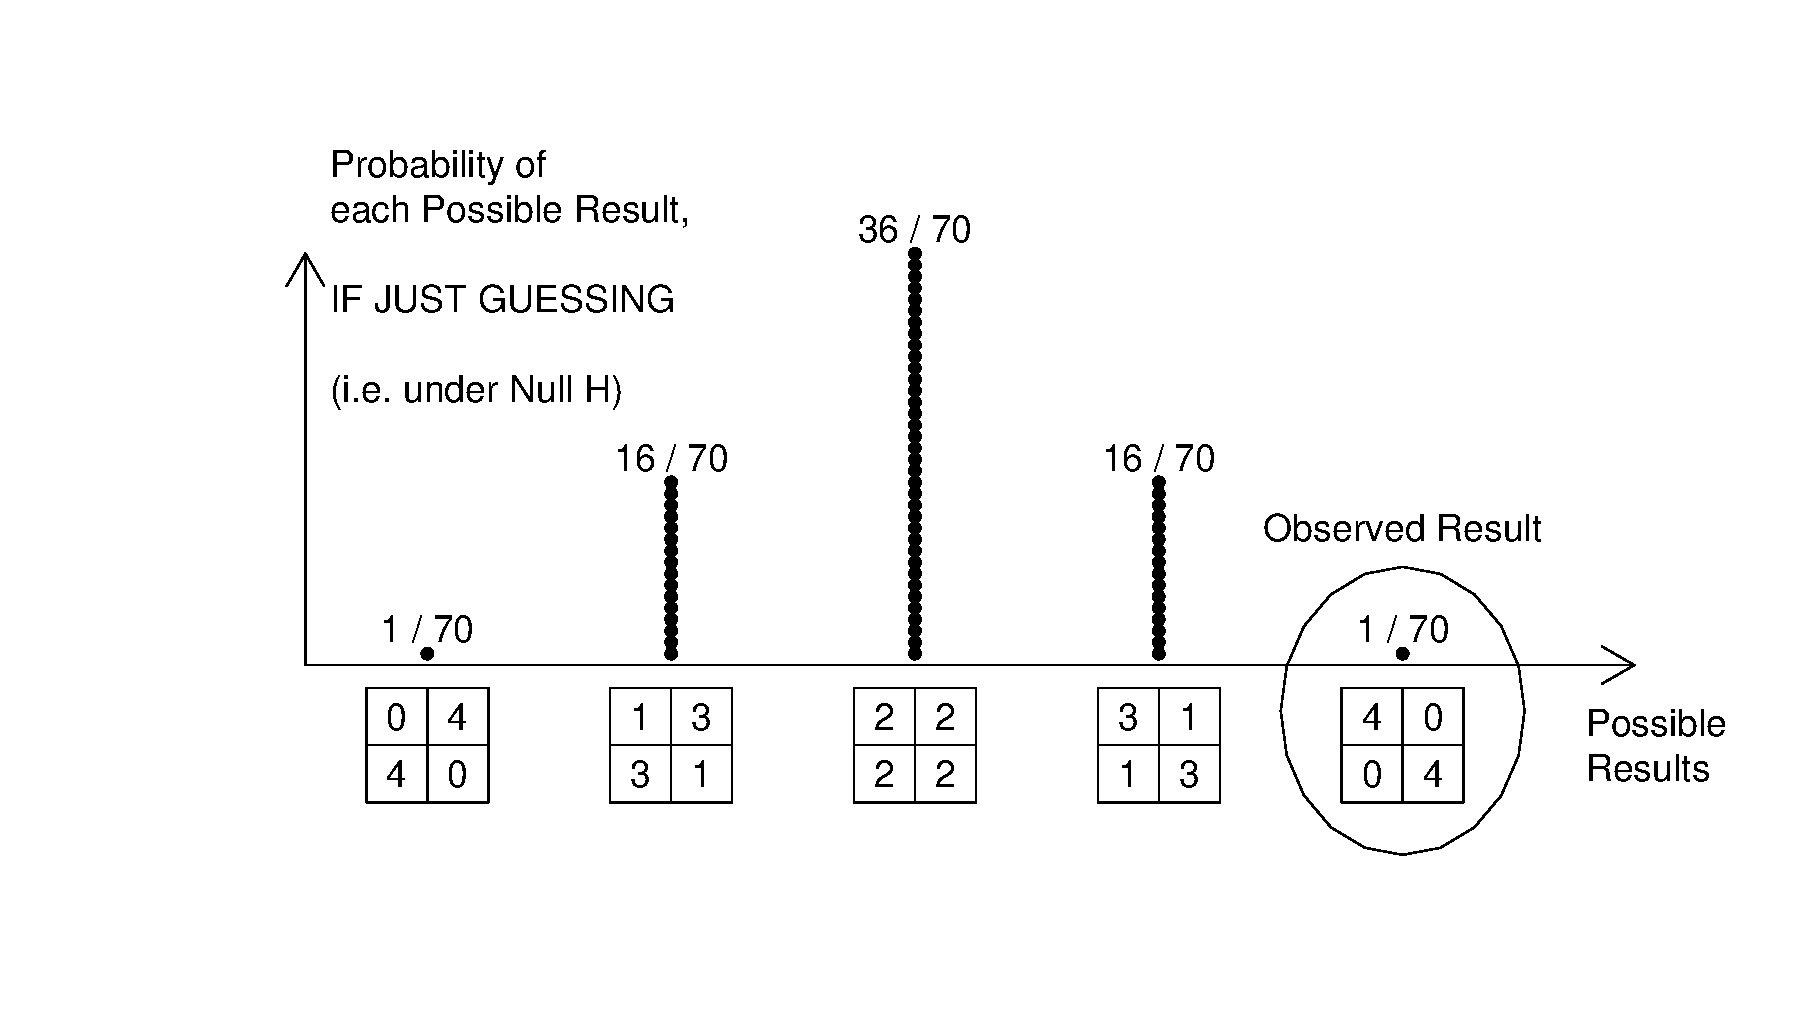
\includegraphics[width=2.5in]{ProbResults.pdf}
\end{center}
\pause
In this example, observed result is the most extreme, so
$$P_{value}=\textrm{Prob[correctly identifying all 4, IF merely guessing]} = 1/70 = 0.014.$$ \pause
\item
Interpretation of such data  often  rather simplistic, as if these \textit{data alone} should \textit{decide}:  i.e. if $P_{value} < 0.05,$ we \sout{`reject' H}$_{null}$; if $P_{value} > 0.05,$ we don't (or worse, we \sout{`accept' H}$_{null}$). Avoid such simplistic `conclusions'.

\end{itemize}
\end{footnotesize}
\end{frame}

\begin{frame}
\frametitle{Example 2 -- Preston-Jones vs. Preston-Jones, English House of Lords, 1949}

\underline{Divorce case:}

\vspace*{.3in}

\begin{itemize}
	\item Sole evidence of adultery was that a baby was born almost 50 weeks after husband had gone abroad on military service.  The appeal failed.
	\item To quote the court: 
	\begin{itemize}
		\item ``\textit{The appeal judges agreed that the limit of credibility had to be drawn somewhere, but on medical 
evidence 349 (days) while improbable, was scientifically possible.}''
	\end{itemize}
\end{itemize}



\end{frame}

\begin{frame}
\frametitle{Example 2 -- data collected from the 1970s}

	\begin{center}
		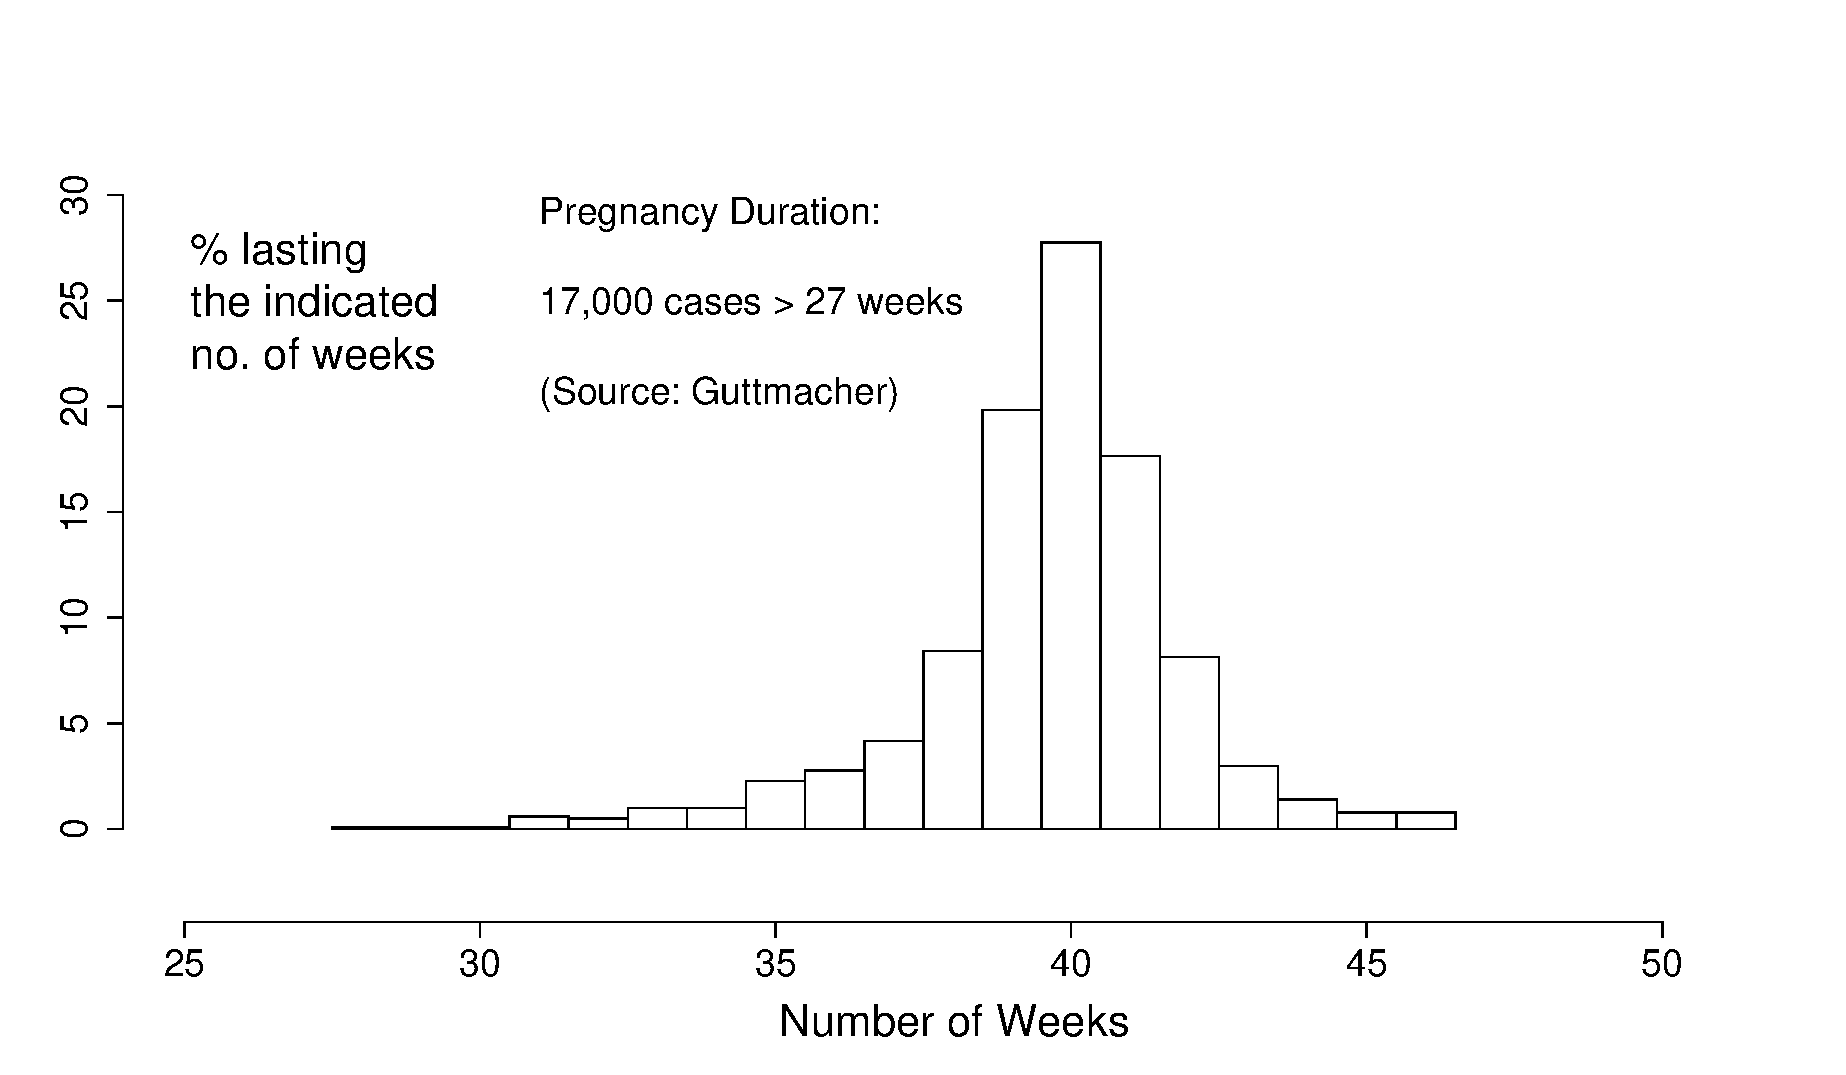
\includegraphics[width=3in]{PregnancyDuration.pdf}
	\end{center}
	
	\begin{itemize}
		\setlength\itemsep{.3em}
		\item $p$-value, calculated under ``Null'' assumption 
	that husband was father,  =  `tail area' or probability corresponding  to an observation
	of `50 or more weeks' in  above distribution 
	
	%\item Effectively asking: \textbf{What \% of reference distribution does observed value exceed?} \pause 
	\item Same system used to report how extreme a lab value is -- are told
	where value is located in distribution of values from  healthy (reference) population.
	\end{itemize} 
	

\end{frame}



\begin{frame}
\frametitle{$p$-value via the Normal (Gaussian) distribution.}

\begin{footnotesize}
\begin{itemize}
\item When judging extremeness of a sample mean or proportion (or  difference between 2 sample means or proportions) calculated from an amount of information that is sufficient for the Central Limit Theorem to apply, one can use Gaussian distribution to readily obtain the $p$-value.
\item Calculate how many standard errors of the statistic, $SE_{statistic},$ the statistic is from where null hypothesis states true value should be.  This ``number of SE's'' is in this situation referred to as a `$Z_{value}$.'
$$Z_{value} = \frac{statistic -  \textrm{its expected value under } H_{null} }{SE_{statistic}}.$$
$p$-value can then be obtained by determining what \% of values in a Normal distribution are as extreme or more extreme than this $Z_{value}.$
\item
If $n$ is small enough that value of $SE_{statistic},$ is itself subject to some 
uncertainty, one would instead refer the ``number of SE's'' to a more appropriate reference distribution, such as Student's $t$- distribution.
\end{itemize}

\end{footnotesize}
\end{frame}

\begin{frame}
\frametitle{More about the $p$-value}

%\begin{footnotesize}
\begin{itemize}
	\setlength\itemsep{.3em}
\item The $p$-value is a \textbf{probability concerning data}, \textbf{conditional on the Null Hypothesis being true}. \pause
\item \textbf{Naive (and not so naive) end-users sometimes interpret the $p$-value  as
the probability that Null Hypothesis is true}, \textit{conditional on -- i.e. given --  the data.} \pause
%\item Very few MDs mix up complement of specificity (i.e. probability of a `positive'  test result when in fact patient does not have disease in question) with positive predictive value (i.e. probability that a patient who has had a `positive'  test result does  have disease in question).
\begin{align*}
p_{value} & = P(\textrm{this or more extreme data}| H_0) \\
& \neq P(H_0|\textrm{this or more extreme data}).
\end{align*}
\item Statistical tests are often coded as statistically significant or not according to whether results are extreme or not with respect to a reference (null)  distribution.  But a test result  is just one piece of data, and needs to be considered \textit{along with  rest of evidence} before coming to a `conclusion.' \item \textbf{Likewise with statistical `tests': the $p$-value is just one more piece of \textit{evidence}, hardly enough to `conclude' anything}. 
%\item The probability that the DNA from the blood  of a randomly selected (innocent) person would match that from blood on crime-scene glove was 
%$p=10^{-17}$. \textit{Do not equate this} Prob[data $|$ innocent] \textit{with its transpose}:
%writing ``data'' as shorthand for ``this or more extreme data'', we need to be aware that 
%$$p_{value} = Prob[ \ data \  | \  H_0 ] \neq Prob[ \ H_0 \  |  \ data ].$$
\end{itemize}
%\end{footnotesize}
\end{frame}

\begin{frame}
\frametitle{The prosecutor's fallacy \footnote{{\tiny Who's the DNA fingerprinting pointing at? New Scientist, 1994.01.29, 51-52.}}}

 \begin{itemize}
 	\setlength\itemsep{1em}
 	\item A criminal leaves fifty thousand blood cells at the scene of a crime which is just barely enough to stain a handkerchief. 
 	\item A forensic scientist extracts DNA from the sample to create a ‘DNA fingerprint’. 
 	\item Its pattern resembles that of a suspect. 
 	\item The scientist calculates that the chance of a match between the sample and a random member of the public is one in a million. How incriminating is this evidence?
 \end{itemize}

\end{frame}

\begin{frame}
\frametitle{The prosecutor's fallacy}

	
	\begin{itemize}
		\item Statistician Peter Donnelly opened a new area of debate, remarking that 

\begin{itemize}
	 	\setlength\itemsep{1em}
	\item \blue{Forensic evidence answers the question}: ``What is the probability that the defendant's DNA profile matches that of the crime sample, assuming that the defendant is innocent?''
			
	\item \blue{While the jury must try to answer the question}: ``What is the probability that the defendant is 		innocent, assuming that the DNA profiles of the defendant and the crime sample match?'' 
\end{itemize}
\pause 
		\item
		The error in mixing up these two probabilities 
		is called ``\textbf{the prosecutor's fallacy},'' 
		and it is suggested that newspapers regularly 
		make this error. 
		\item
		Donnelly's testimony convinced the judges 
		that the case before them involved an example of this and they 
		ordered a retrial.
	\end{itemize}

\end{frame}

\begin{frame}
\frametitle{The prosecutor's fallacy in a game of poker}

\begin{itemize}
		\setlength\itemsep{1em}
		\item  Imagine the judges were playing a game of poker with the Archbishop of Canterbury. 
		\item If the Archbishop were to deal a royal flush on the first hand, one might suspect him of cheating. 
		\item The probability of the Archbishop dealing a royal flush on any one hand, assuming he is an honest card player, is about 1 in 70 000. 
		\item But if the judges were asked whether the Archbishop was honest, given that he had just dealt a royal flush, they would be likely to quote a probability greater than 1 in 70 000. \pause 
		\item The first probability is analogous to the answer of the forensic scientist's
		question, and the second probability analogous to the answer of the jury's
		question. 
\end{itemize}

\end{frame}


\begin{frame}
\frametitle{(Intimate) Relationship between $p$-value and CI}
\begin{center}
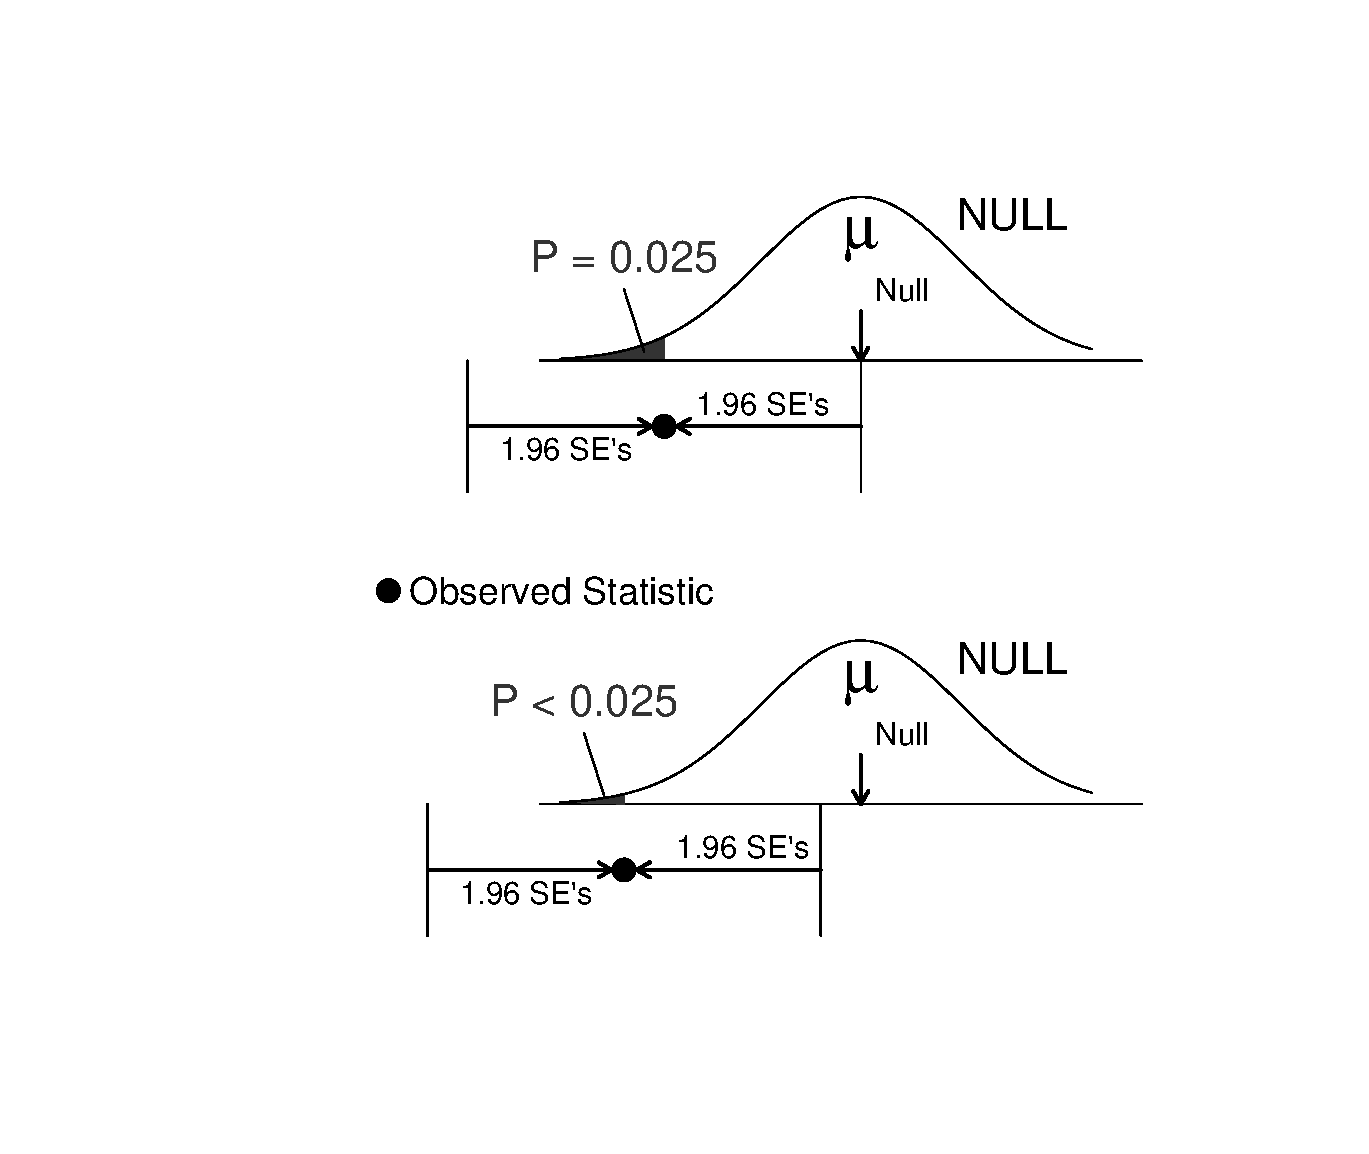
\includegraphics[width=1.65in]{P-CI.pdf}
\end{center} 
\begin{footnotesize}
\begin{itemize}
\item
(Upper graph) If upper limit of 95\% CI\textit{ just touches} null value, then
the 2 sided $p$-value is 0.05 (or 1 sided $p$-value is 0.025). \pause
\item
(Lower graph) If upper limit \textit{excludes} null value, then
the 2 sided $p$-value is less than 0.05 (or 1 sided $p$-value is less than 0.025). \pause
\item
(Graph not shown) If  CI \textit{includes} null value, then the 2-sided $p$-value is greater than (the conventional) 0.05, and thus observed statistic is ``not statistically significantly different'' from hypothesized null value. 
\end{itemize}
\end{footnotesize}
\end{frame}

\begin{frame}
\frametitle{Don't be overly-impressed by $p$-values}
\begin{itemize}
	\setlength\itemsep{0.5em}
\item
$p$-values and `significance tests' widely misunderstood and misused.
\item
Very large or very small $n$'s can influence what is or is not `statistically significant.'
\item
Use CI's instead.
\item
\textit{Pre study} power calculations (the chance that results will be `statistically significant', as a
function of the true underlying difference) of some help.
\item
\textit{post-study} (i.e., \textit{after the data have `spoken'}), a CI is much more relevant,
as it focuses on magnitude \& precision, not on a probability calculated under H$_{null}.$
\end{itemize}
\end{frame}

\section{Applications}


\begin{frame}
\frametitle{Do infant formula samples $\downarrow$ dur$^{n.}$ of breastfeeding?\footnote{{\footnotesize Bergevin Y, Dougherty C, Kramer MS. Lancet. 1983 1(8334):1148-51}}}



Randomized Clinical Trial (RCT) which withheld free formula samples [given by baby-food companies to breast-feeding mothers leaving Montreal General Hospital with their newborn infants] from a random half of those studied.

\begin{scriptsize}
\begin{center}
\begin{tabular}{|c c c c c| l|}
\hline
& \multicolumn{2}{c}{Mothers}  & & & \\
At 1 month & given & not given & Total  & $ \ $ &  \\
& sample & sample & & & \textbf{Conclusion...} \\ 
\hline
Still Breast & 175 & 182 & 357 & & \\ 
feeding & (\textbf{\textit{77\%}}) & (\textbf{\textit{84\%}}) & (80.4\%) & 
& P=0.07. So, ...  \\ 
& & & & & the difference is   \\
Not Breast & 52 & 35 & 87  &  &  ``Not Statistically \\ 
feeding &  & & & &  Significant" at 0.05 level  \\
\hline
Total & 227 & 217 &  444 & & \\
\hline
\end{tabular}
\end{center}
\end{scriptsize}

\begin{center}
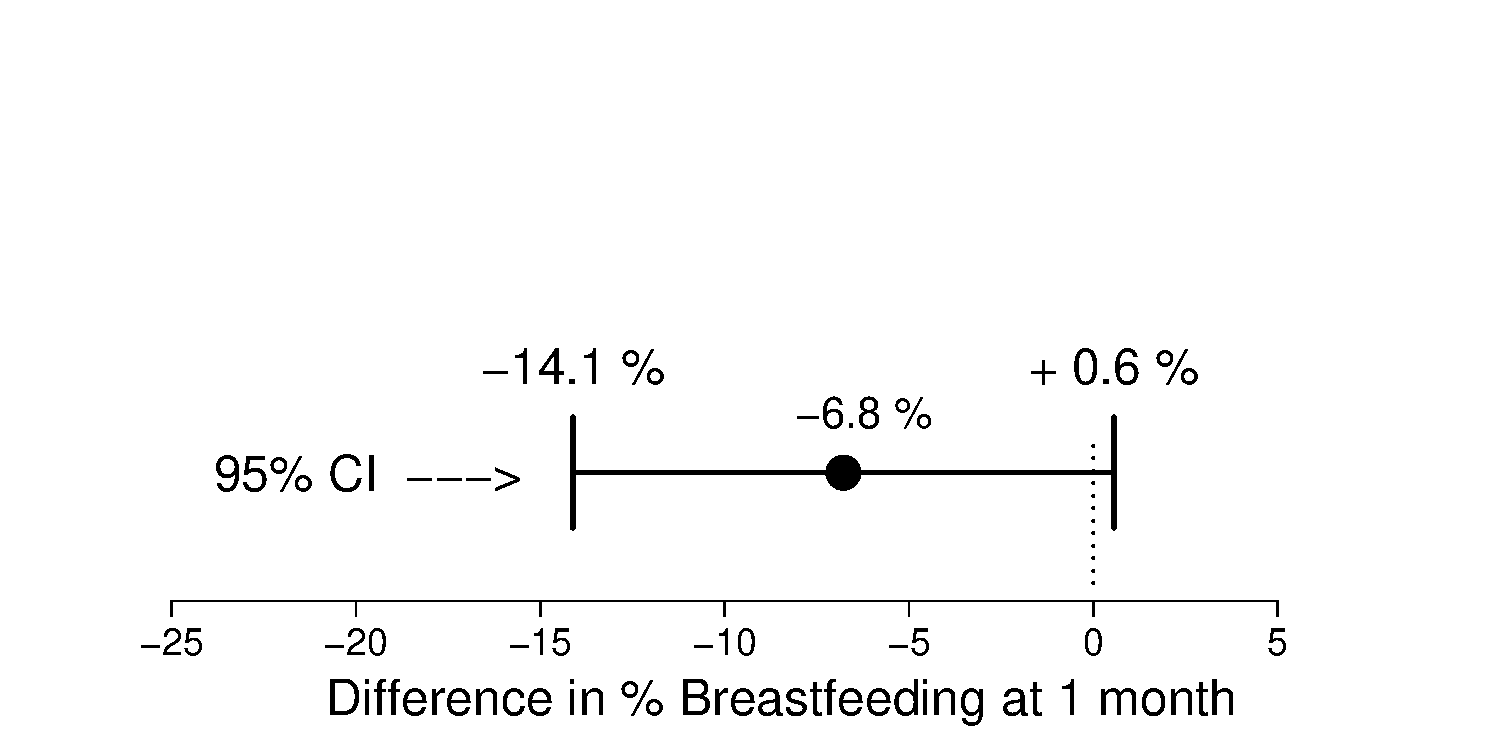
\includegraphics[width=1.75in]{Bergevin.pdf}
\end{center}

\end{frame}

\begin{frame}
\frametitle{Messages}

\begin{small}
\begin{itemize}
		\setlength\itemsep{0.5em}
	
\item \lowercase{NO MATTER WHETHER THE $p$-value IS ``STATISTICALLY SIGNIFICANT'' OR NOT,
ALWAYS LOOK AT THE LOCATION AND WIDTH OF THE CONFIDENCE INTERVAL. IT
GIVES YOU A BETTER AND MORE COMPLETE INDICATION OF THE MAGNITUDE OF
THE EFFECT AND OF THE PRECISION WITH WHICH IT WAS MEASURED.
\item
THIS IS AN EXAMPLE OF AN \textbf{INCONCLUSIVE NEGATIVE} STUDY, SINCE IT 
HAS \textbf{INSUFFICIENT PRECISION} (``RESOLVING POWER") \textbf{TO DISTINGUISH} BETWEEN TWO IMPORTANT POSSIBILITIES -- \textbf{NO HARM}, AND WHAT AUTHOROTIES WOULD CONSIDER A \textbf{SUBSTANTIAL HARM: A REDUCTION OF 10 PERCENTAGE POINTS} IN BREASTFEEDING RATES . 
\item
``\textbf{STATISTICALLY} SIGNIFICANT`` AND ``\textbf{CLINICALLY}-'' (OR ``\textbf{PUBLIC HEALTH}-'') SIGNIFICANT ARE DIFFERENT CONCEPTS.   

\item
(Message from 1st author:) Plan to have \textbf{enough statistical power}. His study had only 50\% power to detect a difference of 10 percentage points)}

\end{itemize}
\end{small}
\end{frame}

\begin{frame}
\frametitle{Do starch blockers really block calorie absorption?}

{\scriptsize Starch blockers -- their effect on calorie absorption from a high-starch meal.
Bo-Linn GW. et al New Eng J Med. 307(23):1413-6, 1982 Dec 2}

\begin{footnotesize}

\begin{itemize}
\item
Known for more than 25 years that certain plant foods, e.g., kidney beans \& wheat, contain a substance that inhibits activity of salivary and pancreatic amylase.
\item
More recently, this antiamylase has been purified and marketed for use in weight control under generic name ``starch blockers.'' 
\item
Although this approach to weight control is highly popular, it has never been shown whether starch-blocker tablets actually reduce  absorption of calories from starch.
\item
Using a one-day calorie-balance technique and a high starch (100 g) meal (spaghetti, tomato sauce, and bread), we measured excretion of fecal calories after $n=5$ normal subjects in a cross-over trial had taken either placebo or starch-blocker tablets.
\item
If the starch-blocker tablets had prevented the digestion of starch, fecal calorie excretion should have increased by 400 kcal.
\end{itemize}
\end{footnotesize}
\end{frame}

\begin{frame}
\frametitle{Do starch blockers really block calorie absorption?}

\begin{itemize}
\item
However, fecal calorie excretion was same on the 2 test days (mean $\pm$ S.E.M., 80 $\pm$ 4 as compared with 78 $\pm$ 2).
\begin{center}
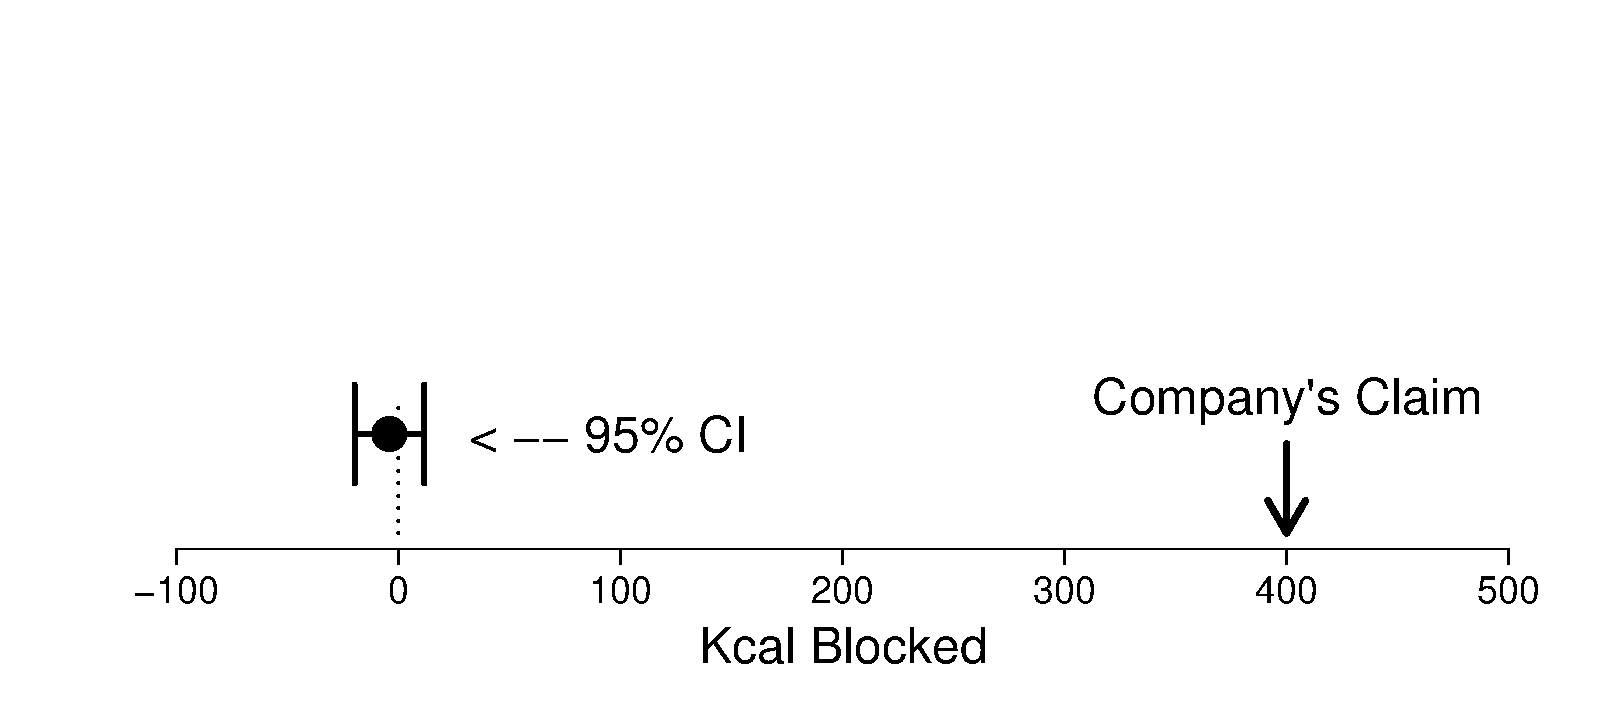
\includegraphics[width=4in]{StarchBlockers.pdf}
\end{center}
\item
We conclude that starch blocker tablets do not inhibit the digestion and absorption of starch calories in human beings.
\item
EFFECT IS MINISCULE (AND ESTIMATE QUITE PRECISE) 
AND VERY FAR FROM COMPANY'S CLAIM !!! 
\item
A `\textbf{DEFINITIVELY NEGATIVE}' STUDY.
\end{itemize}
\end{frame}

\section{Summary}
\begin{frame}
\frametitle{SUMMARY - 1}
\begin{itemize}
			\setlength\itemsep{1em}
%\item The difference sources of variability have important implications in patient management.
%\item Descriptive statistics should be descriptive, and should suit the pattern of variation.
\item Confidence intervals  preferable to $p$-values, since they are expressed in terms of (comparative) parameter of interest;  they allow us to judge magnitude and its precision, and help  us in
`ruling in / out'  certain parameter values. 
\item
A `statistically significant' difference does not necessarily imply a clinically important difference.
\item
A `not-statistically-significant' difference does not necessarily imply that we have ruled out a clinically important difference. 
\end{itemize}
\end{frame}

\begin{frame}
\frametitle{SUMMARY - 2}
\begin{itemize}
				\setlength\itemsep{.51em}
\item
Precise estimates  distinguish b/w that which --  if it were true  -- would be important and that which --  if it were true  --  would not. `$n$'  an important determinant of precision.
\item A lab value in upper 1\% of reference distribution  (of values derived from people  without known diseases/conditions )  does not mean that there is a 1\% chance that person in whom it was measured is healthy; i.e., it doesn't mean that there's a 99\% chance that the person in whom it was measured  does have some disease/condition.
\item Likewise,  $p$-value $\neq$ probability that null hypothesis is true.
\item
The fact that 
$$Prob[ the \ data \ | \ Healthy ]\textrm{  is small [or large]}$$
does not necessarily mean that
$$Prob[ Healthy \ | \ the \ data ]\textrm{  is small [or large]}$$
\end{itemize}
\end{frame}

\begin{frame}
\frametitle{SUMMARY - 3}
\begin{itemize}
\item
Ultimately, $p$-values, CI's and other evidence from a study need to be combined with other information bearing on  parameter or process. \newline
\item
Don't treat any one study as last word on the topic. \newline
%\item
%Worry also about distortions of a non-sampling kind that are not minimized by having a large `$n$.' A larger sample size will not reduce  systematic differences in a comparison. \newline
\end{itemize}
\end{frame}


\section{Power and Sample Size}

\frame{\frametitle{Is this milk watered down?\footnote{\scriptsize{Adapted from Q 15.17 from Moore and McCabe, 4th Edition}}}


\begin{itemize}
	\item A cheese maker buys milk from several suppliers. It suspects that some suppliers are adding water to their milk to increase their profits.
	\item Excess water can be detected by measuring the freezing point of the liquid. \pause
	\item The freezing temperature of natural milk varies according to a Gaussian distribution, with mean $\mu =  -0.540^{\circ}$ Celsius (C) and standard deviation $\sigma =0.008^{\circ}$C. 
	\item Added water raises the freezing temperature toward $0^{\circ}$C, the freezing point of water. \pause
	\item The laboratory manager measures the freezing temperature of five consecutive lots of `milk' from one supplier. The mean of these 5 measurements is -0.533$^{\circ}$C. \pause
	\item \blue{Question:} Is this good evidence that the producer is adding water to the milk? 
\end{itemize}

%\textit{Moore and McCabe} asked students to `State hypotheses, carry out the test, give the P -value, and state your conclusion.'
}

\begin{frame}[fragile]{Is this milk watered down?}
	\begin{itemize}
		\setlength\itemsep{.7em}
		\item \blue{State hypotheses:} \pause \begin{itemize}
			\item $H_0: \mu =  -0.540^{\circ}$C \pause
			\item  $H_a: \mu >  -0.540^{\circ}$C
		\end{itemize}
		\item Which test should we use and why? \pause \\ \ \\

		
\begin{knitrout}\scriptsize
\definecolor{shadecolor}{rgb}{0.969, 0.969, 0.969}\color{fgcolor}
\begin{alltt}
\hlstd{mosaic}\hlopt{::}\hlkwd{xpnorm}\hlstd{(}\hlkwc{q} \hlstd{=} \hlopt{-}\hlnum{0.533}\hlstd{,} \hlkwc{mean} \hlstd{=} \hlopt{-}\hlnum{0.540}\hlstd{,} \hlkwc{sd} \hlstd{=} \hlnum{0.008}\hlopt{/}\hlkwd{sqrt}\hlstd{(}\hlnum{5}\hlstd{))}
\end{alltt}


{\ttfamily\noindent\itshape\color{messagecolor}{\#\# }}

{\ttfamily\noindent\itshape\color{messagecolor}{\#\# If X \textasciitilde{} N(-0.54, 0.003578), then}}

{\ttfamily\noindent\itshape\color{messagecolor}{\#\# 	P(X <= -0.533) = P(Z <= 1.957) = 0.9748}}

{\ttfamily\noindent\itshape\color{messagecolor}{\#\# 	P(X >\ \ -0.533) = P(Z >\ \ 1.957) = 0.0252}}

{\ttfamily\noindent\itshape\color{messagecolor}{\#\# }}

{\centering 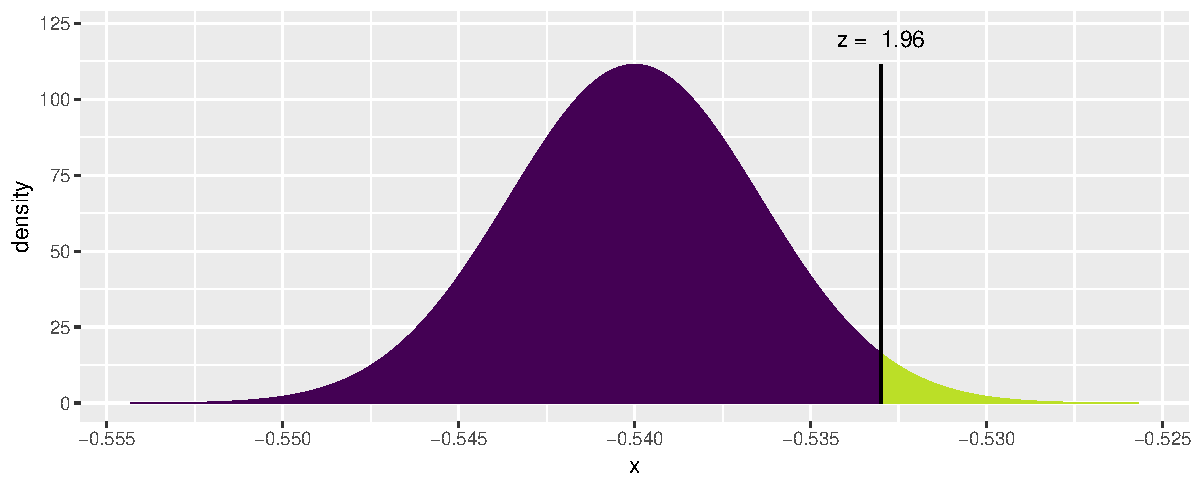
\includegraphics[width=1\linewidth]{figure/unnamed-chunk-1-1} 

}


\begin{verbatim}
## [1] 0.9748004
\end{verbatim}

\end{knitrout}

\end{itemize}
\end{frame}

\begin{frame}[fragile]{Testing using the $p$-value}
Appropriate wordings to accompany $p=0.0252$:
\begin{itemize}
	\setlength\itemsep{1.5em}
	\item If we test samples of \underline{pure milk}, only 2.6\% of test results would be this high or higher.
	\pause 
	\item \underline{IF} the \underline{only} factor operating here were sampling variation, only  2.6\% of test results on pure milk  \underline{would be} this high or higher.
\end{itemize}

\end{frame}

\begin{frame}[fragile]{Test using a $Z$ statistic}
\begin{itemize}
	\setlength\itemsep{.7em}
	\item   $H_0: \mu =  -0.540^{\circ}$C $\qquad$  $H_a: \mu >  -0.540^{\circ}$C
	
	\item We can also standardize our observed mean and calculate the $p$-value under a $\mathcal{N}(0,1)$ \\ \ \\

\begin{knitrout}\scriptsize
\definecolor{shadecolor}{rgb}{0.969, 0.969, 0.969}\color{fgcolor}
\begin{alltt}
\hlstd{SEM} \hlkwb{<-} \hlnum{0.008}\hlopt{/}\hlkwd{sqrt}\hlstd{(}\hlnum{5}\hlstd{)}
\hlstd{z_stat} \hlkwb{<-} \hlstd{(}\hlopt{-}\hlnum{0.533} \hlopt{-} \hlstd{(}\hlopt{-}\hlnum{0.540}\hlstd{))} \hlopt{/} \hlstd{SEM}
\hlstd{mosaic}\hlopt{::}\hlkwd{xpnorm}\hlstd{(}\hlkwc{q} \hlstd{= z_stat,} \hlkwc{mean} \hlstd{=} \hlnum{0}\hlstd{,} \hlkwc{sd} \hlstd{=} \hlnum{1}\hlstd{)}
\end{alltt}


{\ttfamily\noindent\itshape\color{messagecolor}{\#\# }}

{\ttfamily\noindent\itshape\color{messagecolor}{\#\# If X \textasciitilde{} N(0, 1), then}}

{\ttfamily\noindent\itshape\color{messagecolor}{\#\# 	P(X <= 1.957) = P(Z <= 1.957) = 0.9748}}

{\ttfamily\noindent\itshape\color{messagecolor}{\#\# 	P(X >\ \ 1.957) = P(Z >\ \ 1.957) = 0.0252}}

{\ttfamily\noindent\itshape\color{messagecolor}{\#\# }}

{\centering 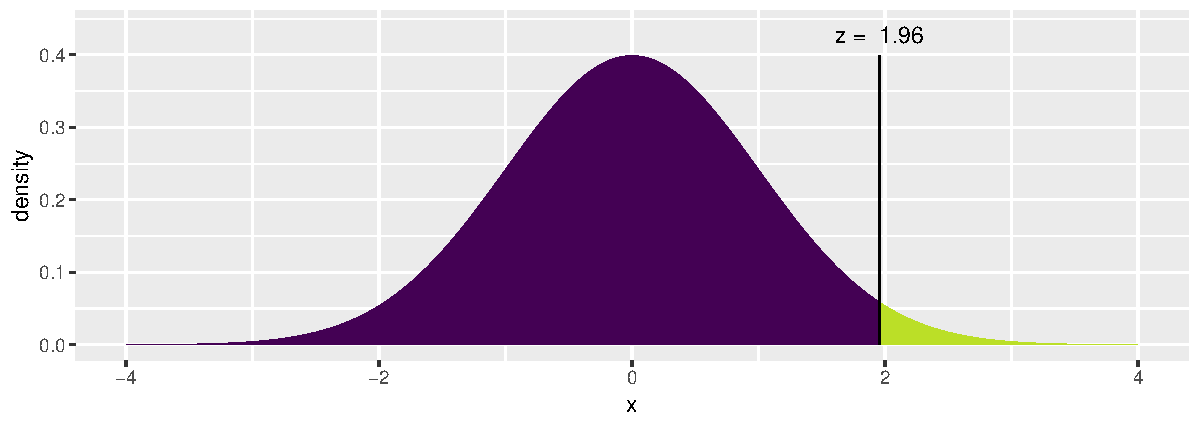
\includegraphics[width=1\linewidth]{figure/unnamed-chunk-2-1} 

}


\begin{verbatim}
## [1] 0.9748004
\end{verbatim}

\end{knitrout}
	
\end{itemize}
\end{frame}


\begin{frame}[fragile]{Test using critical values}
\begin{itemize}

	\item An observed mean freezing temperature greater than -0.5341 rejects the null hypothesis:
	
\begin{knitrout}\scriptsize
\definecolor{shadecolor}{rgb}{0.969, 0.969, 0.969}\color{fgcolor}
\begin{alltt}
\hlstd{mosaic}\hlopt{::}\hlkwd{xqnorm}\hlstd{(}\hlkwc{p} \hlstd{=} \hlnum{0.95}\hlstd{,} \hlkwc{mean} \hlstd{=} \hlopt{-}\hlnum{0.540}\hlstd{,} \hlkwc{sd} \hlstd{=} \hlnum{0.008}\hlopt{/}\hlkwd{sqrt}\hlstd{(}\hlnum{5}\hlstd{))}
\end{alltt}


{\ttfamily\noindent\itshape\color{messagecolor}{\#\# }}

{\ttfamily\noindent\itshape\color{messagecolor}{\#\# If X \textasciitilde{} N(-0.54, 0.003577709), then}}

{\ttfamily\noindent\itshape\color{messagecolor}{\#\# 	P(X <= -0.5341152) = 0.95}}

{\ttfamily\noindent\itshape\color{messagecolor}{\#\# 	P(X >\ \ -0.5341152) = 0.05}}

{\ttfamily\noindent\itshape\color{messagecolor}{\#\# }}

{\centering 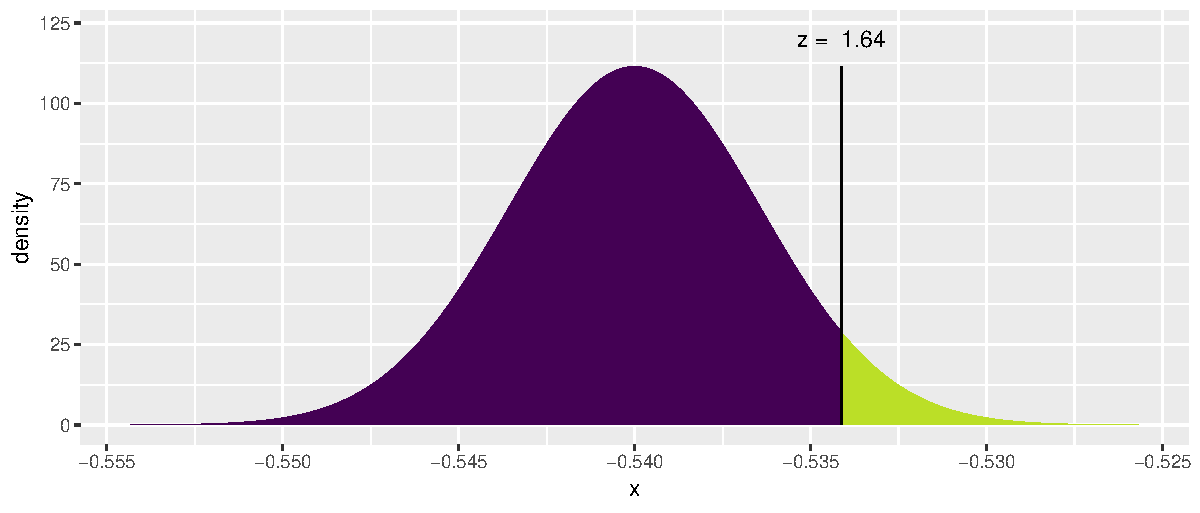
\includegraphics[width=1\linewidth]{figure/unnamed-chunk-3-1} 

}


\begin{verbatim}
## [1] -0.5341152
\end{verbatim}

\end{knitrout}

	
\end{itemize}
\end{frame}

\begin{frame}[fragile]{Test using critical values}


	\begin{minipage}{0.47\textwidth}
\begin{knitrout}\scriptsize
\definecolor{shadecolor}{rgb}{0.969, 0.969, 0.969}\color{fgcolor}
\begin{alltt}
\hlstd{mosaic}\hlopt{::}\hlkwd{xqnorm}\hlstd{(}\hlkwc{p} \hlstd{=} \hlnum{0.95}\hlstd{,}
\hlkwc{mean} \hlstd{=} \hlopt{-}\hlnum{0.540}\hlstd{,}
\hlkwc{sd} \hlstd{=} \hlnum{0.008}\hlopt{/}\hlkwd{sqrt}\hlstd{(}\hlnum{5}\hlstd{))}
\end{alltt}
\begin{figure}

{\centering 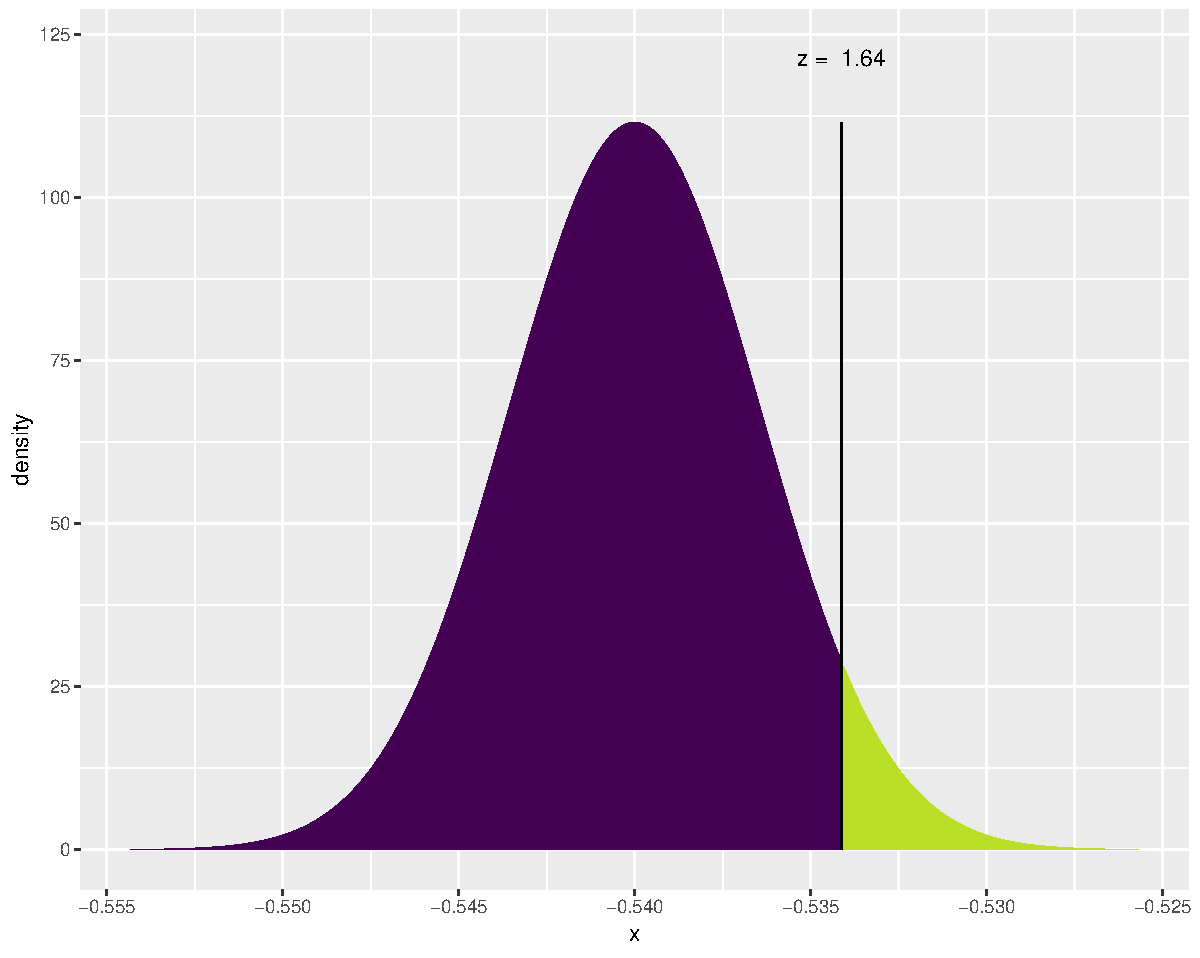
\includegraphics[width=1\linewidth]{figure/unnamed-chunk-4-1} 

}

\caption[critical value under the null distribution]{critical value under the null distribution}\label{fig:unnamed-chunk-4}
\end{figure}


\end{knitrout}
	\end{minipage}
	\begin{minipage}{0.47\textwidth}
\begin{knitrout}\scriptsize
\definecolor{shadecolor}{rgb}{0.969, 0.969, 0.969}\color{fgcolor}
\begin{alltt}
\hlstd{mosaic}\hlopt{::}\hlkwd{xpnorm}\hlstd{(}\hlkwc{q} \hlstd{=} \hlopt{-}\hlnum{0.533}\hlstd{,}
\hlkwc{mean} \hlstd{=} \hlopt{-}\hlnum{0.540}\hlstd{,}
\hlkwc{sd} \hlstd{=} \hlnum{0.008}\hlopt{/}\hlkwd{sqrt}\hlstd{(}\hlnum{5}\hlstd{))}
\end{alltt}
\begin{figure}

{\centering 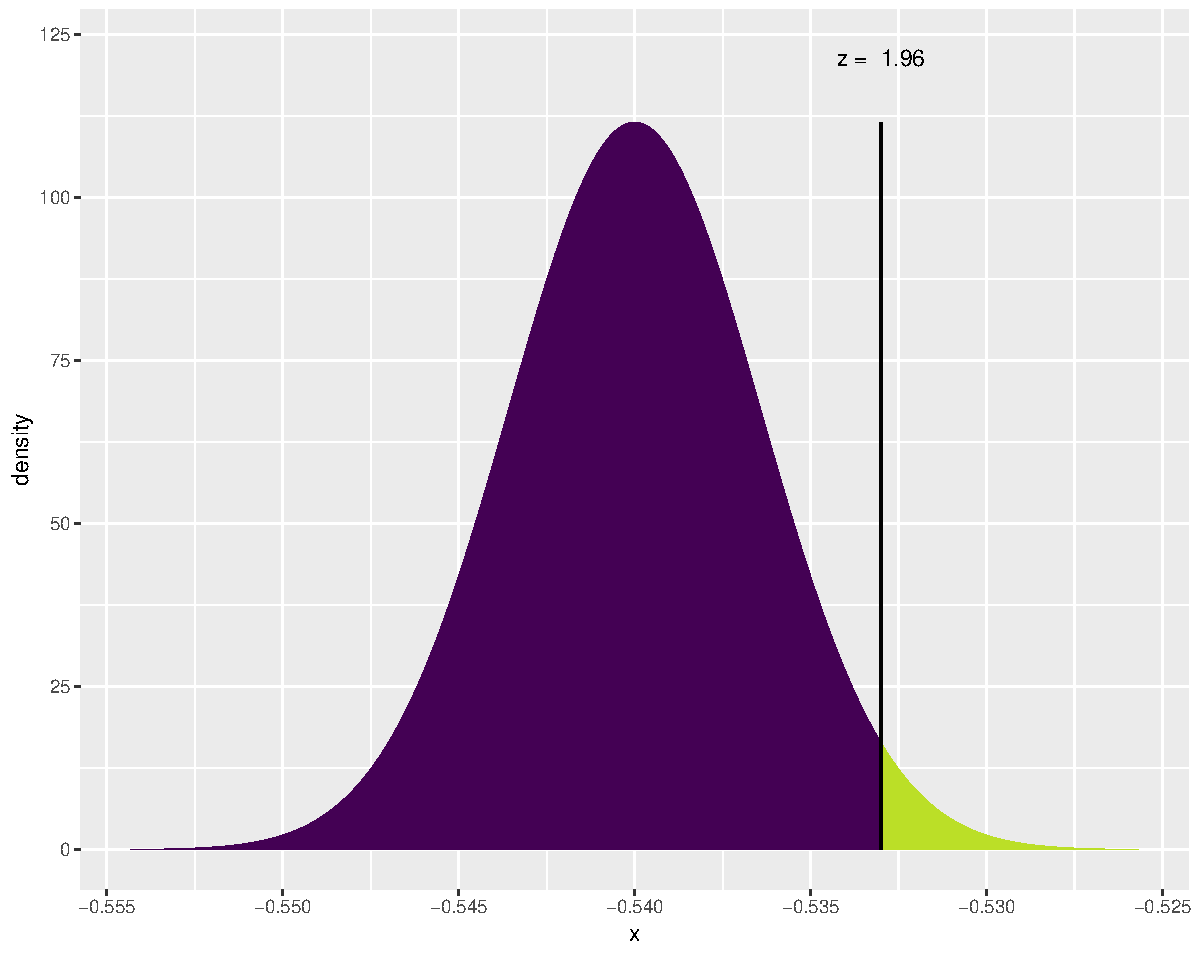
\includegraphics[width=1\linewidth]{figure/unnamed-chunk-5-1} 

}

\caption[test statistic under the null distribution]{test statistic under the null distribution}\label{fig:unnamed-chunk-5}
\end{figure}


\end{knitrout}
\end{minipage}	
	
Thus we reject $H_0$ at $\alpha = 0.05$.
\end{frame}

\frame{\frametitle{Type I and II errors} What does it mean to reject
	$H_0$ at level $\alpha$? \pause 
	\begin{itemize}
		\item It means that, if $H_0$ were true and the procedure (sampling data,
		performing the significance test) were repeated many times, the
		testing procedure would reject $H_0$ $\alpha100$\% of the time.
	\end{itemize}
\centering
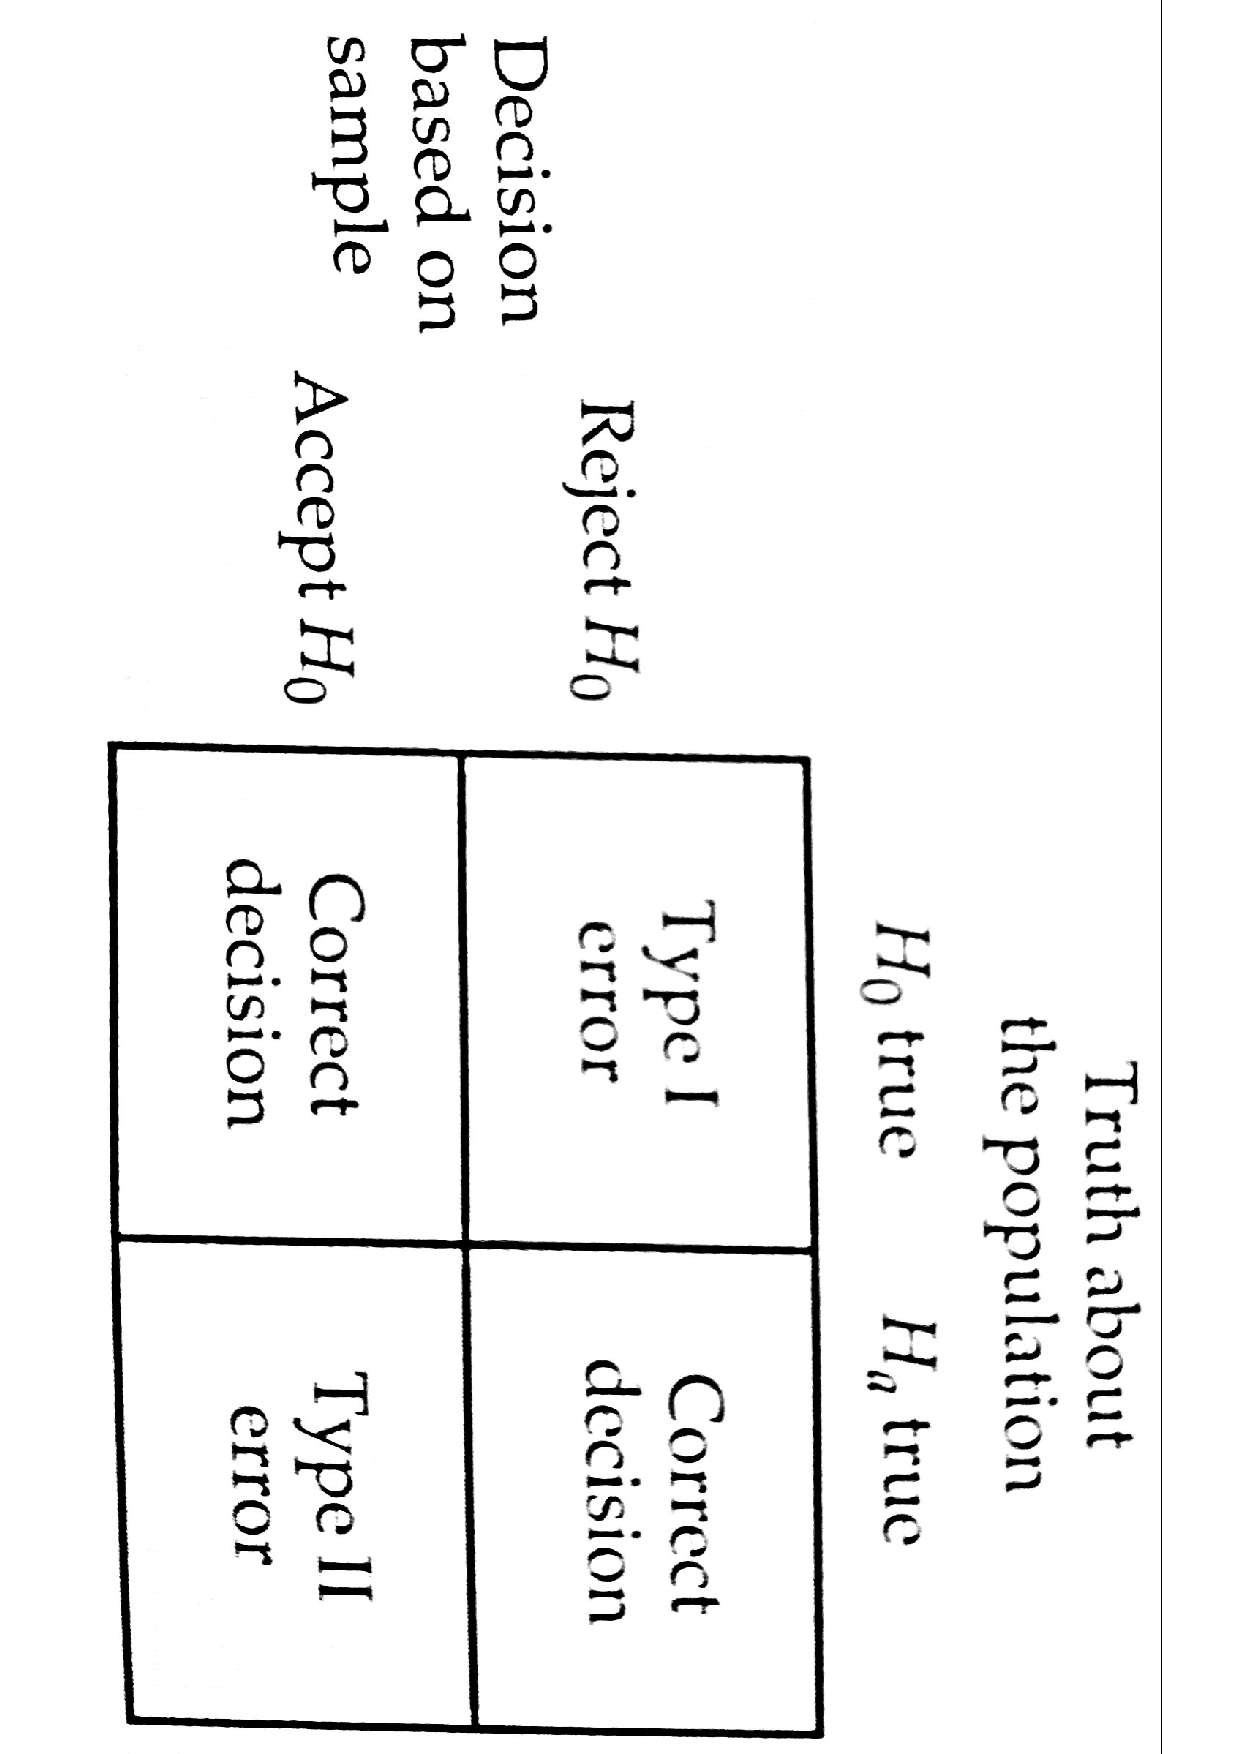
\includegraphics[angle=90, scale=0.25]{type1.pdf}

} \frame{\frametitle{Type I and II errors} In this special setting
	we give special names to the false positive and false negative
	rates:
	\begin{itemize}
		\item \textbf{Type I error ($\alpha$):} probability that a significance test will
		reject $H_0$ when in fact $H_0$ is true. \pause
		\item \textbf{Type II error ($\beta$):} probability that a significance test will
		fail to reject $H_0$ when $H_0$ is not true.
		\item[]
	\end{itemize}
\pause 
	The Type I error is the significance level of the test, $\alpha$,
	which is often set to 0.05. \\ \ \\
	As we will see in a moment, the Type II error, $\beta$, is
	determined by the sample size and the chosen Type I error
	rate/significance level. (Therefore, with $\alpha$ fixed at, say
	0.05, the only way to reduce $\beta$ is to increase $n$ or decrease
	$s$.)}

\frame{\frametitle{Type I and II errors}
	\begin{figure}
		\begin{center}
			\epsfig{figure=HypTest1.pdf,width=4.2in,height=3.4in}
		\end{center}
	\end{figure}
} \frame{\frametitle{Type I and II errors}
	\begin{figure}
		\begin{center}
			\epsfig{figure=HypTest2.pdf,width=4.2in,height=3.4in}
		\end{center}
	\end{figure}
} 

\frame{\frametitle{Type I and II errors}
\small
\begin{itemize}
	\item \pause[2] The blue area represents the Type I error -- the probability of
	rejecting $H_0$ \textbf{if $H_0$ is true}.
	\item \pause[3] The purple area represents the Type II error -- the probability of
	\textit{not} rejecting $H_0$ \textbf{if $H_A$ is in fact true} (and therefore $H_0$
	should be rejected). 
\end{itemize}

\vspace*{-0.2in}

\pause[1]
\begin{figure}
	\begin{center}
		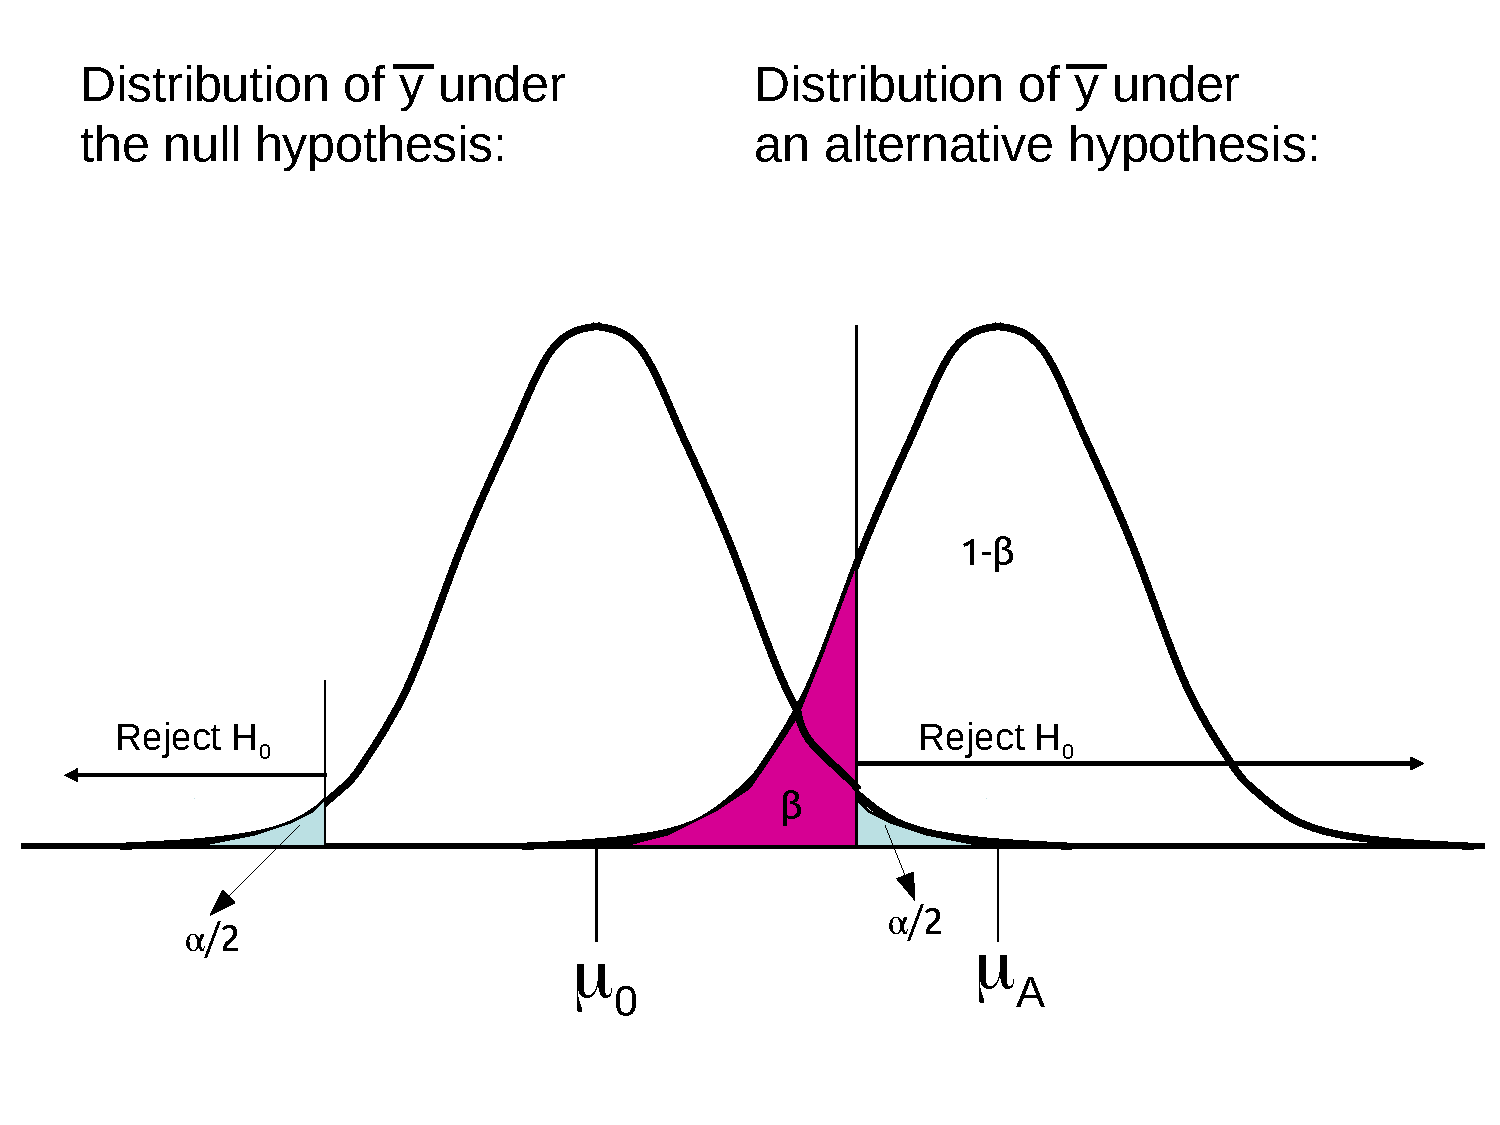
\includegraphics[scale=0.30]{HypTest3-2.pdf}
	\end{center}
\end{figure}
} 


\begin{frame}[fragile]{Type I and II errors}
\small
\begin{itemize}
	%\item the variability of the sampling distribution of $\overline{y}$ 
	\item Notice the distribution of the alternative has a different center, but the same SD  \pause 
	\item The distance between $\mu_0$ and the true value of $\mu$ (in our previous slide we called this $\mu_A$) will affect the Type II error. This distance is denoted as $\Delta$.
\end{itemize}


\centering
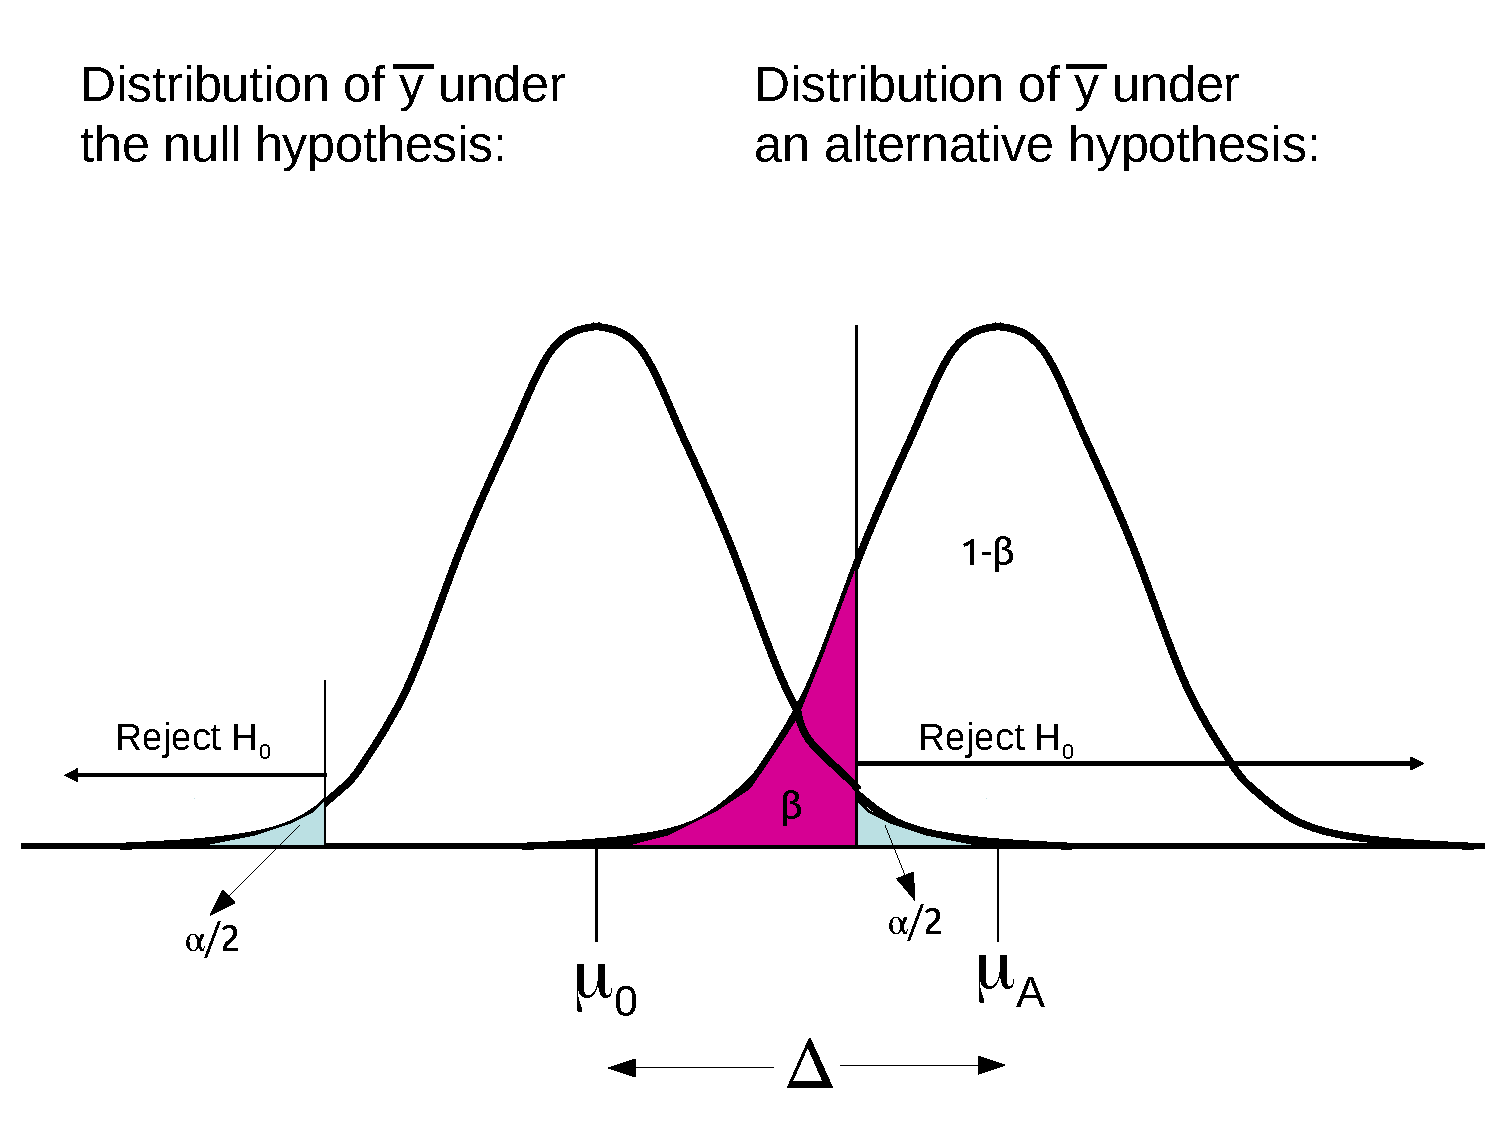
\includegraphics[scale=0.30]{HypTest3-3.pdf}



\end{frame}


\begin{frame}[fragile]{Power = $1 - \beta$}

\vspace*{-0.2in}

\begin{defm}[Power = $1-\beta$]
	The probability that a fixed level $\alpha$ significance test will reject $H_0$ when a particular alternative value of the parameter is true is called the \textbf{power} of the test to detect the alternative. 
\end{defm}


\vspace*{-0.08in}

\centering
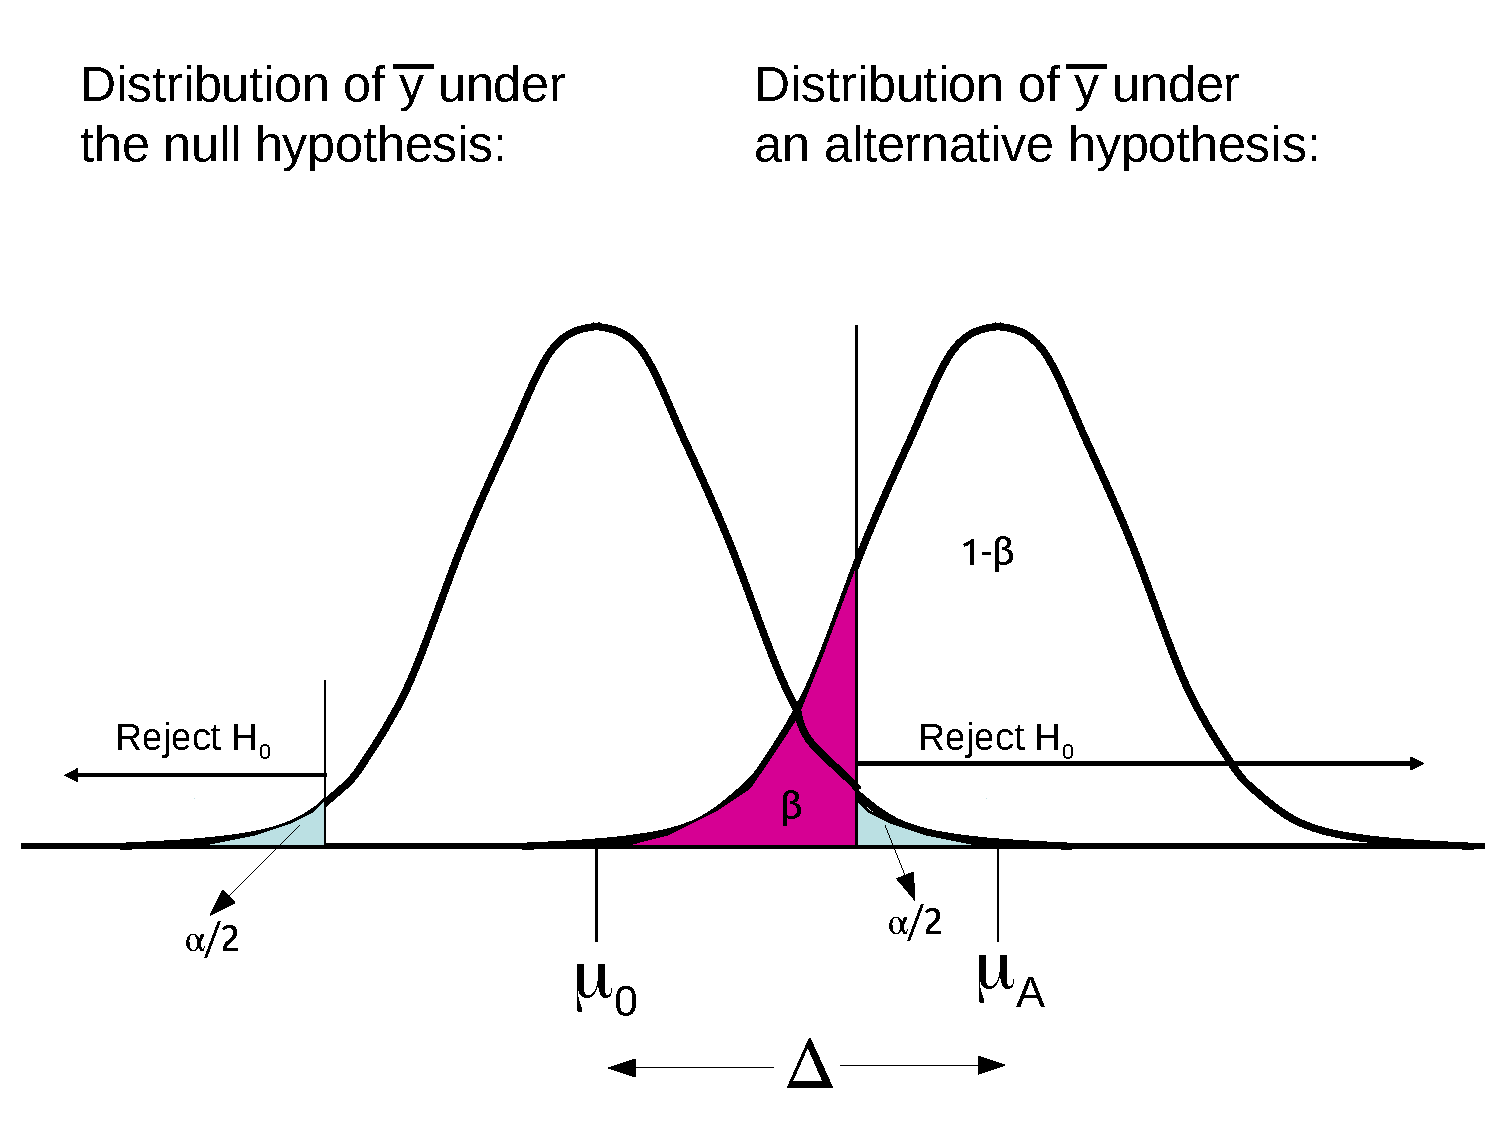
\includegraphics[scale=0.31]{HypTest3-3.pdf}


\end{frame}




\begin{frame}{Power and Sample Size: 3 questions}

\begin{enumerate}
	\setlength\itemsep{1em}
	\item How much water a supplier could add to the milk before they have a 10\% , 50\%, 80\%
	chance of getting caught, i.e., of the buyer detecting the cheating ? \pause
	\item Assume a 99:1 mix of milk and water. What are the chances of detecting cheating if the buyer uses samples $n$=10, 15 or 20 rather than just 5 measurements? \pause
	\item At what $n$ does the chance of detecting cheating reach 80\%? (\textit{a commonly used, but arbitrary, criterion used in sample-size planning by investigators seeking funding for their proposed research})
	\end{enumerate}

\end{frame}


\section{How much water a supplier could add to the milk before they have a 10\% , 50\%, 80\% chance of getting caught, i.e., of the buyer detecting the cheating ?}

\begin{frame}{Statistical Power: the chance of getting caught}
\begin{itemize}
	\setlength\itemsep{1em}
	\item We want to know how much water a farmer could add to the milk before they have a 10\% , 50\%, 80\% chance of getting caught (of the buyer detecting the cheating). 
	\item Assume the buyer continues to use an $n=5$, and the same $\sigma =0.008^{\circ}$C, and  bases the boundary for rejecting/accepting the product on a $\alpha = 0.05$, and a 1-sided test which translates to the buyer setting the cutoff at $$-0.540 + 1.645 \times 0.008/\sqrt{5}  = -0.534^{\circ}\textrm{C}.$$
	\item This is equivalent to \texttt{qnorm(p = 0.95, mean = -0.540, sd = 0.008/sqrt(5))}
\end{itemize}
\end{frame}

\begin{frame}[fragile]{The cutoff at $\alpha = 0.05$}
\begin{itemize}
	\item $-0.540 + 1.645 \times 0.008/\sqrt{5}  = -0.534^{\circ}\textrm{C}.$
\end{itemize}

\begin{knitrout}\scriptsize
\definecolor{shadecolor}{rgb}{0.969, 0.969, 0.969}\color{fgcolor}
\begin{alltt}
\hlstd{mosaic}\hlopt{::}\hlkwd{xqnorm}\hlstd{(}\hlkwc{p} \hlstd{=} \hlnum{0.95}\hlstd{,} \hlkwc{mean} \hlstd{=} \hlopt{-}\hlnum{0.540}\hlstd{,} \hlkwc{sd} \hlstd{=} \hlnum{0.008}\hlopt{/}\hlkwd{sqrt}\hlstd{(}\hlnum{5}\hlstd{))}
\end{alltt}


{\centering 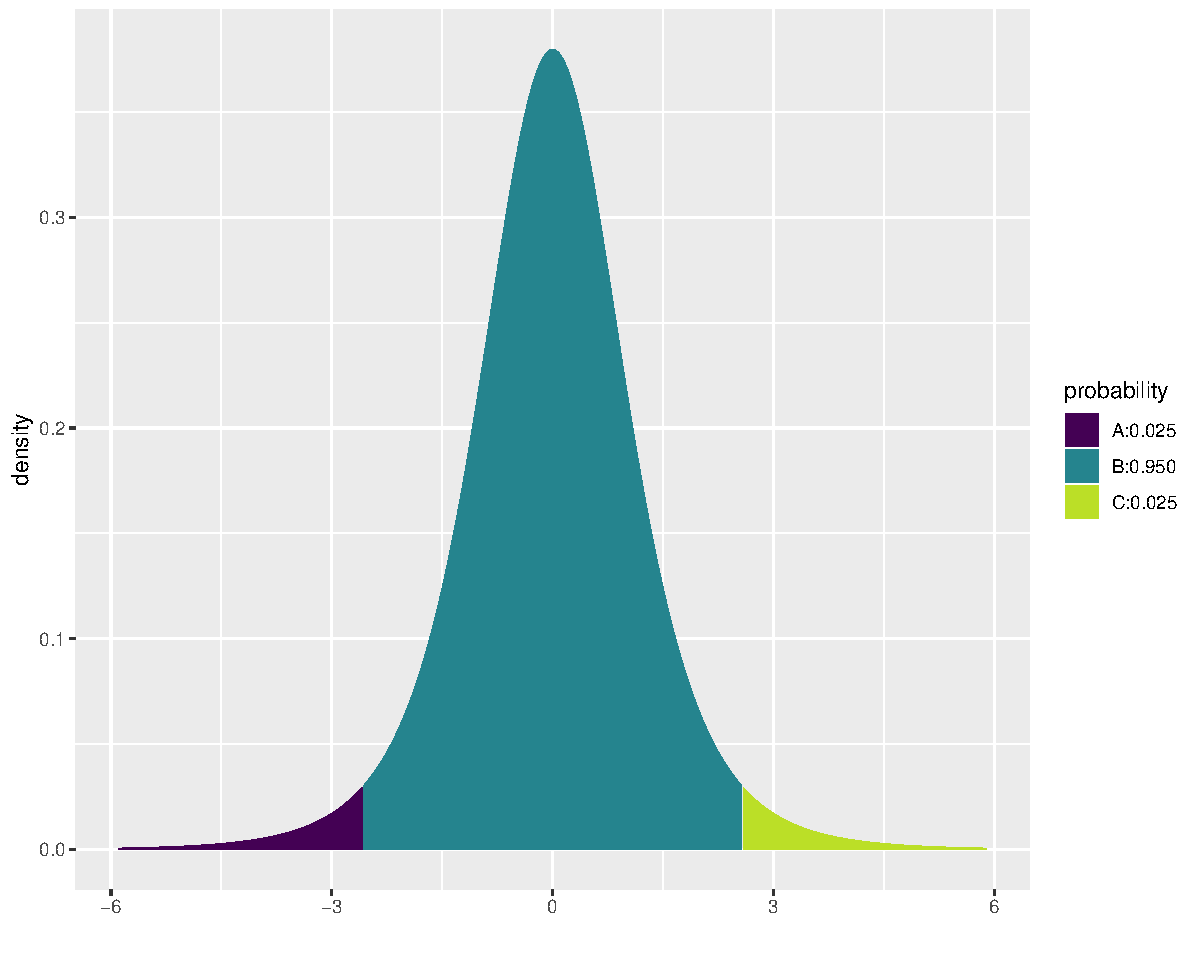
\includegraphics[width=1\linewidth]{figure/unnamed-chunk-6-1} 

}


\begin{verbatim}
## [1] -0.5341152
\end{verbatim}

\end{knitrout}
\end{frame}



\begin{frame}{Statistical Power}
\small
\begin{itemize}
	\setlength\itemsep{1em}
	\item Assume that  mixtures of M\% milk and W\% water  would freeze at a mean of $$\mu_{mixture} =  (M/100) \times -0.545^{\circ}C + (W/100) \times 0 ^{\circ}C$$ and that the $\sigma$ would remain unchanged. \pause 
	\item Thus, mixtures of 99\% milk and 1\% water  would freeze at a mean of $\mu =  (99/100) \times -0.540^{\circ}C + (1/100) \times 0 ^{\circ}C = -0.5346 ^{\circ} C.$ 
	\end{itemize}

\begin{center}
	\begin{tabular}{|c|c|c|}
		\hline 
		\% milk & \% water & mean ($\mu$) \\ 
		\hline 
		99 & 1 & -0.5346$^{\circ}C$ \\ 
		98 & 2 & -0.5292$^{\circ}C$ \\ 
		97 & 3 & -0.5238$^{\circ}C$ \\ 
		\hline 
	\end{tabular} 
\end{center}
\end{frame}


\begin{frame}[fragile]{If the supplier added 1\% water to the milk}
\begin{knitrout}\scriptsize
\definecolor{shadecolor}{rgb}{0.969, 0.969, 0.969}\color{fgcolor}

{\centering 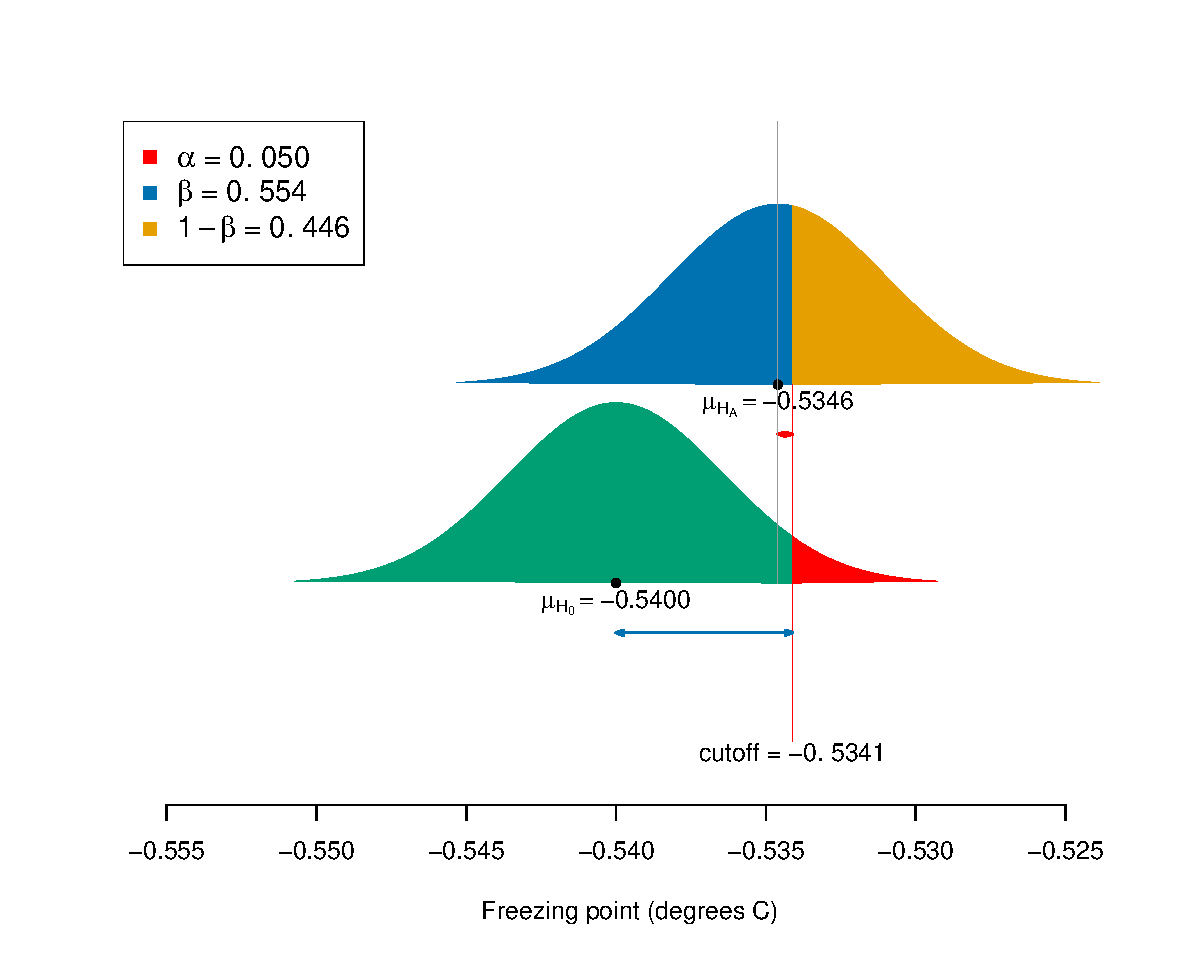
\includegraphics[width=1\linewidth]{figure/unnamed-chunk-7-1} 

}



\end{knitrout}
\end{frame}


\begin{frame}[fragile]{If the supplier added 2\% water to the milk}
\begin{knitrout}\scriptsize
\definecolor{shadecolor}{rgb}{0.969, 0.969, 0.969}\color{fgcolor}

{\centering 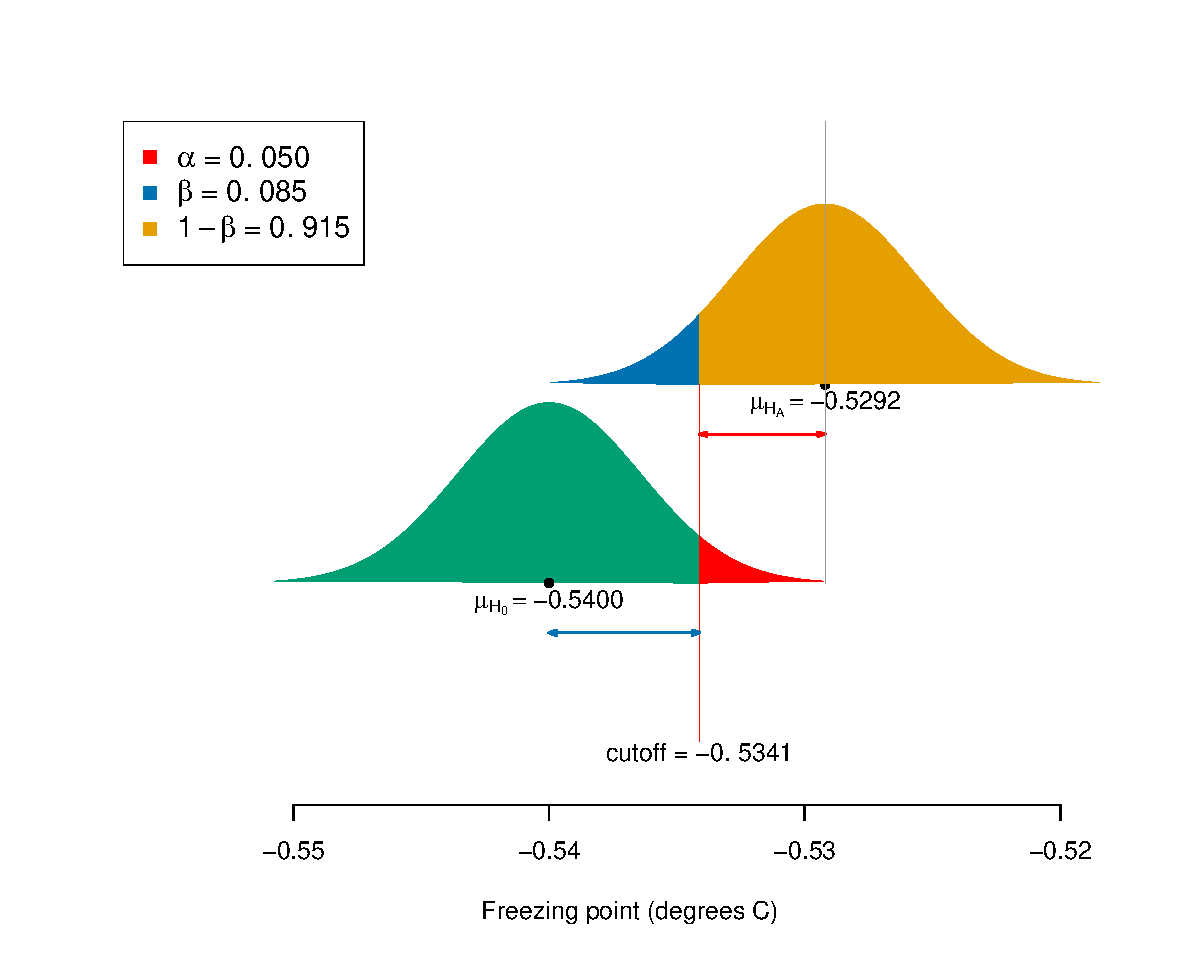
\includegraphics[width=1\linewidth]{figure/unnamed-chunk-8-1} 

}



\end{knitrout}
\end{frame}

\begin{frame}[fragile]{If the supplier added 3\% water to the milk}
\begin{knitrout}\scriptsize
\definecolor{shadecolor}{rgb}{0.969, 0.969, 0.969}\color{fgcolor}

{\centering 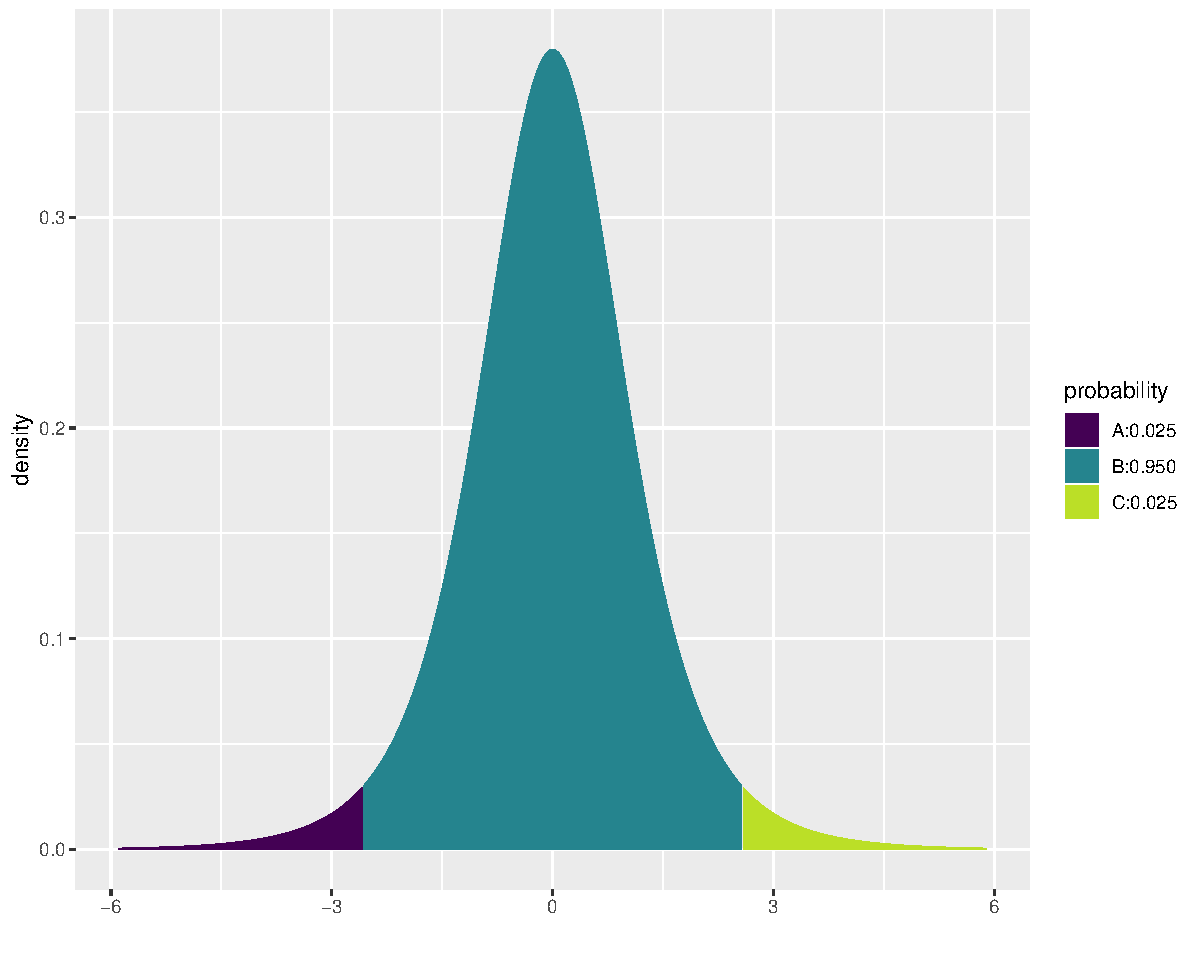
\includegraphics[width=1\linewidth]{figure/unnamed-chunk-9-1} 

}



\end{knitrout}
\end{frame}



\begin{frame}

\begin{center}
	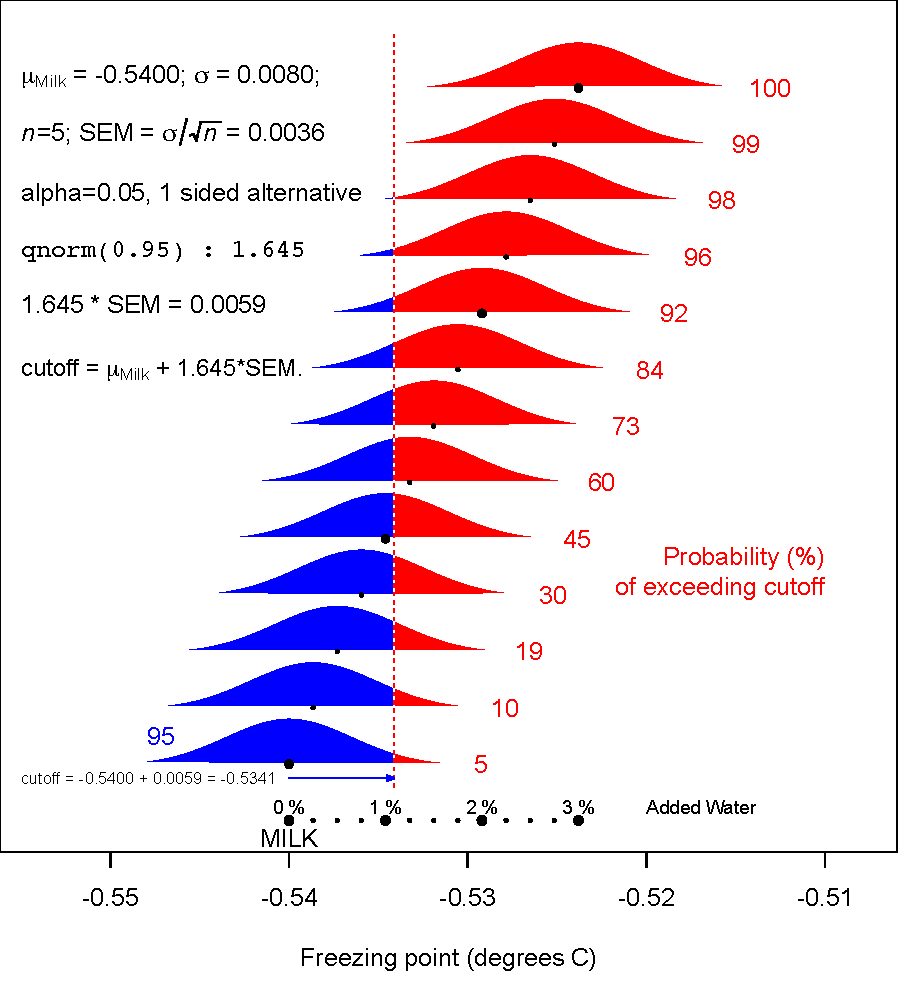
\includegraphics[scale=0.45]{ProbDetectingWaterInMilk.pdf} 
\end{center}

\vspace*{-0.18in}

{ \footnotesize
	The probabilities in red were calculated using the formula:
	\texttt{stats::pnorm(cutoff, mean = mu.mixture, sd = SEM, lower.tail=FALSE)}
}
\end{frame}


\begin{frame}{Statistical Power: the chance of getting caught}
\begin{itemize}
		\setlength\itemsep{1em}
	\item The calculations shown at the left in the figure on the previous slide are used to set  the cutoff; it is based on the \underline{\textbf{null}} distribution shown at the bottom. \pause  
\item Clearly the bigger the signal (the `$\Delta$') the more chance the test will `raise the red flag.' It is 92\% when it is a 98:2, and virtually 100\% when it is a 97:3 mix.
\end{itemize}


\end{frame}


\section{Assume a 99:1 mix of milk and water. What are the chances of detecting cheating if the buyer uses samples $n$=10, 15 or 20 rather than just 5 measurements?}

\begin{frame}{Power as a function of sample size}

\begin{itemize}
	\setlength\itemsep{1em}
	\item Suppose even a 1\% added water is serious, and worth detecting.
\item Clearly, from the previous Figure, and again at the bottom row of the following Figure,
one has only a 45\% chance of detecting it: there is a \textbf{large overlap between the sampling distributions under the null (100\% Milk) and the mixture (99\% milk, 1\% water) scenarios}. \pause 

\item So, to better discriminate, one needs to make a bigger resting effort, and measure more lots,
i.e., increase the $n$.
\end{itemize}
\end{frame}


\begin{frame}[fragile]{When the buyer uses samples of size 5}
\begin{knitrout}\scriptsize
\definecolor{shadecolor}{rgb}{0.969, 0.969, 0.969}\color{fgcolor}

{\centering 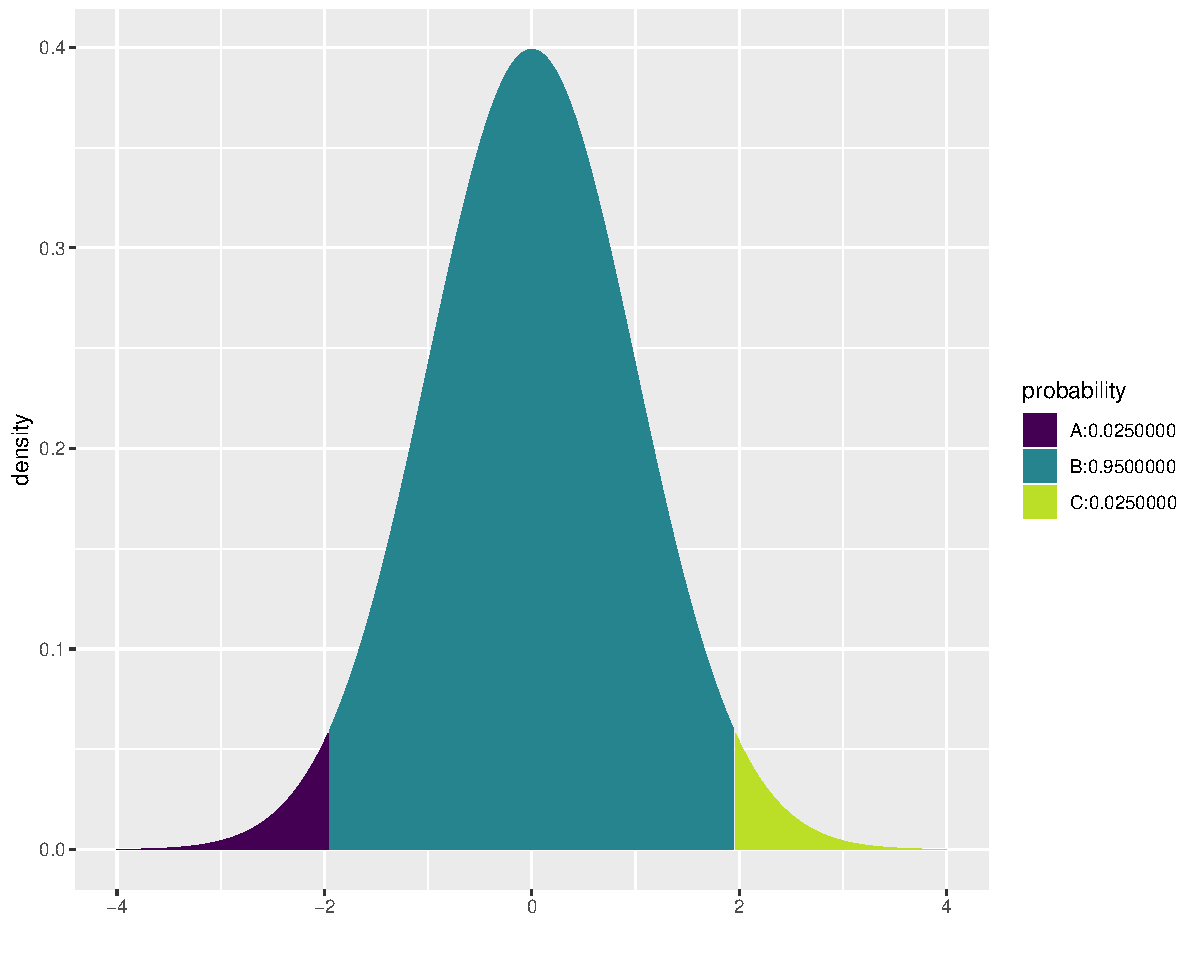
\includegraphics[width=1\linewidth]{figure/unnamed-chunk-10-1} 

}



\end{knitrout}
\end{frame}


\begin{frame}[fragile]{When the buyer uses samples of size 10}
\begin{knitrout}\scriptsize
\definecolor{shadecolor}{rgb}{0.969, 0.969, 0.969}\color{fgcolor}

{\centering 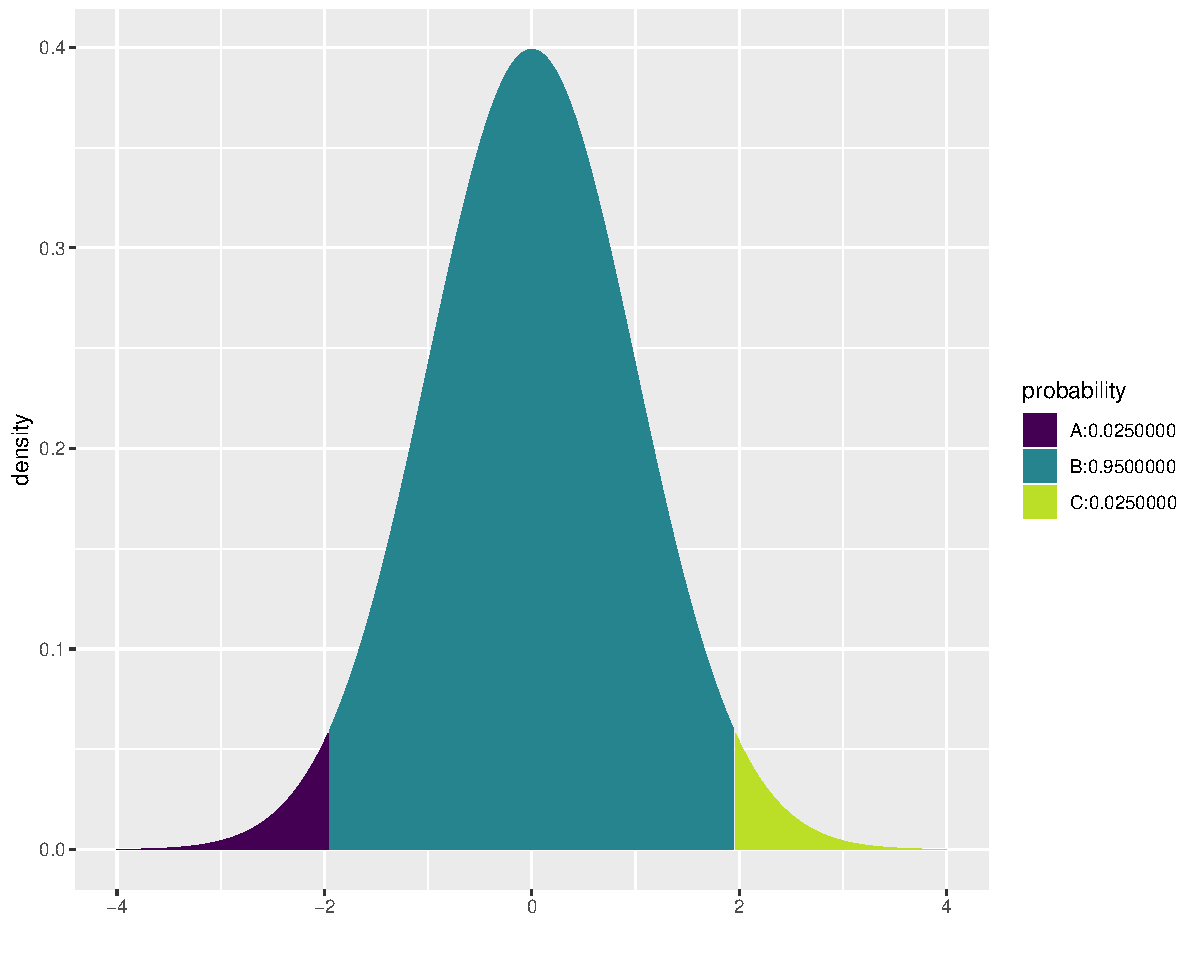
\includegraphics[width=1\linewidth]{figure/unnamed-chunk-11-1} 

}



\end{knitrout}
\end{frame}

\begin{frame}[fragile]{When the buyer uses samples of size 15}
\begin{knitrout}\scriptsize
\definecolor{shadecolor}{rgb}{0.969, 0.969, 0.969}\color{fgcolor}

{\centering 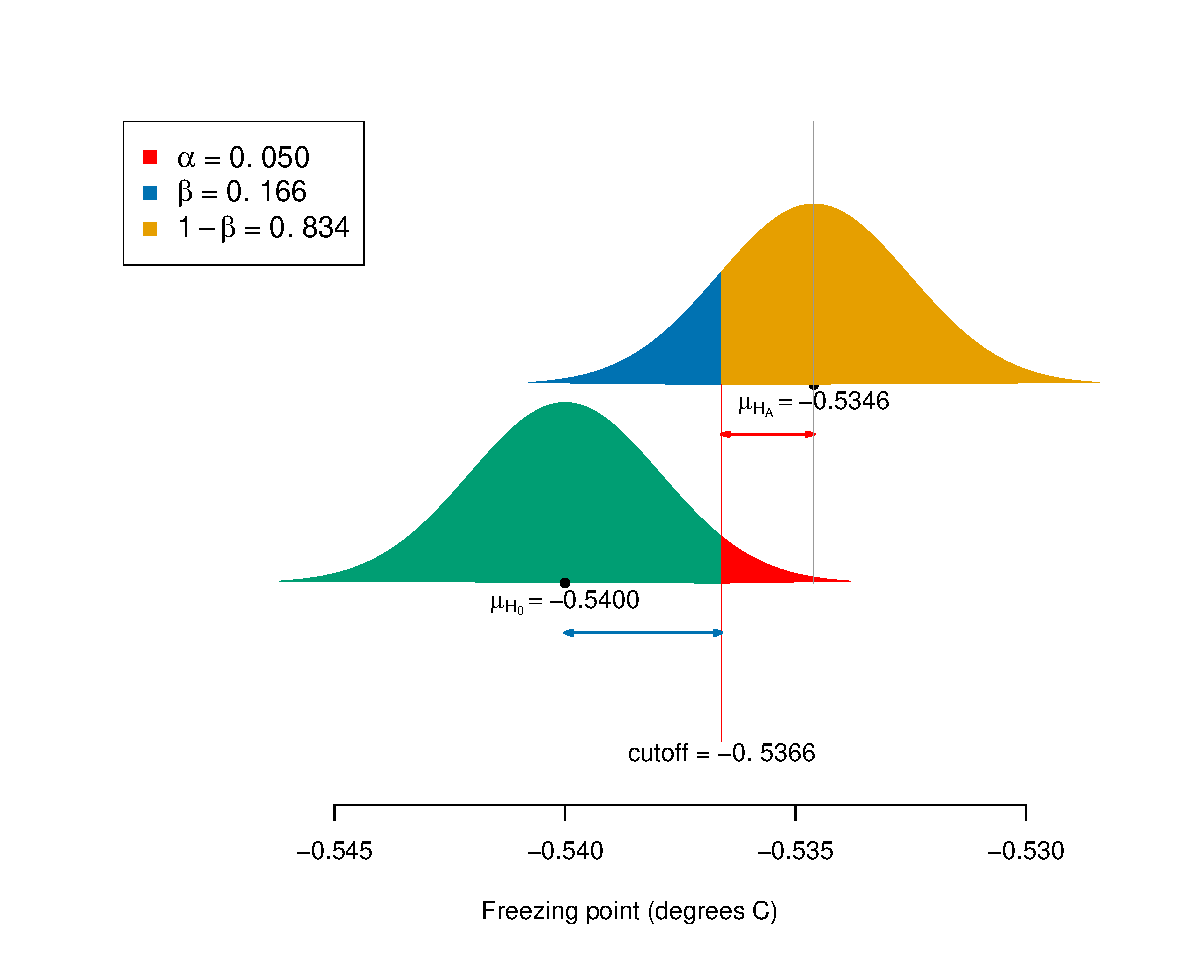
\includegraphics[width=1\linewidth]{figure/unnamed-chunk-12-1} 

}



\end{knitrout}
\end{frame}


\begin{frame}
\begin{center}
	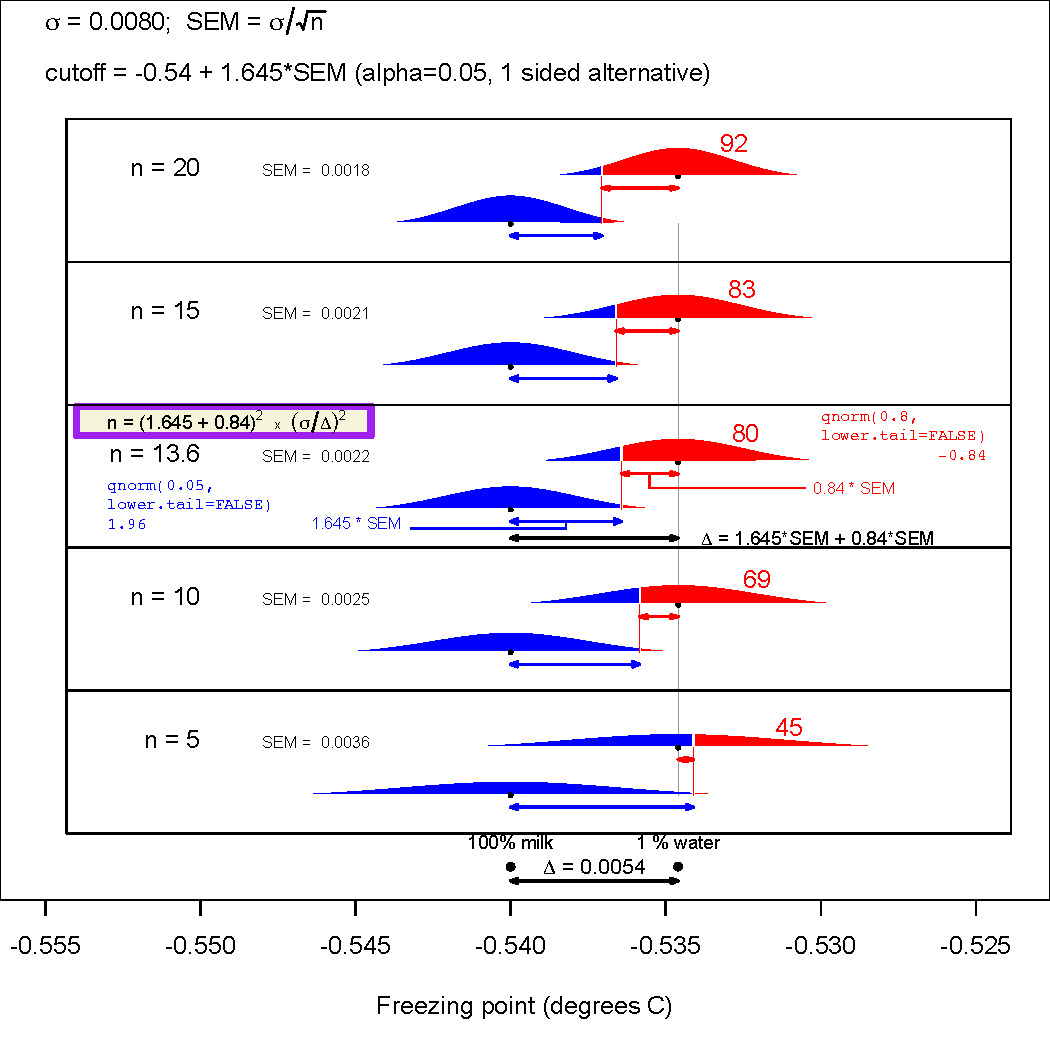
\includegraphics[scale=0.5]{SampleSize1pctWaterAdded.pdf} 
\end{center}
\end{frame}


\begin{frame}{Increasing $n$ leads to increased power}
\begin{itemize}
	\item The larger $n$ narrows and concentrates the sampling distribution. The width is governed by the SD of the sampling distribution of the mean of $n$ measurements, i.e., by the Standard Error of the Mean, or SEM = $\sigma/\sqrt{n}$.\pause 

\item Because the null sampling distribution narrows, the cutoff is brought closer to the null.
And under the alternative (non-null) scenario, a greater portion of its sampling distribution is to
the right of (i.e., exceeds) the cutoff. \pause 

\item Indeed, under the alternative (i.e., cheating) scenario the probability of exceeding the threshold  is almost 70\% when $n=10,$ 82\% when $n=15$ and 92\% when n=20. \pause 
\item 
You can check these for yourself in \texttt{R} using this expression:\\ \ \\
{ \footnotesize
	\ \ \ \ \texttt{\textbf{stats::pnorm(cutoff, mean = mu.mixture, sd = sigma/sqrt(n), lower.tail=FALSE)} }  \\ \ \\
} 
\end{itemize}
\end{frame}


\section{At what $n$ does the chance of detecting cheating reach 80\%?}

\begin{frame}{What sample size needed?}

\begin{itemize}
	\item We can come up with a closed form formula that (a) allows you to compute the sample size `by hand' and (b) shows you, more explicitly than the diagram or R code can, what drives the $n$.

\end{itemize}

\end{frame}

\begin{frame}[fragile]{The balancing formula}
\begin{knitrout}\scriptsize
\definecolor{shadecolor}{rgb}{0.969, 0.969, 0.969}\color{fgcolor}

{\centering 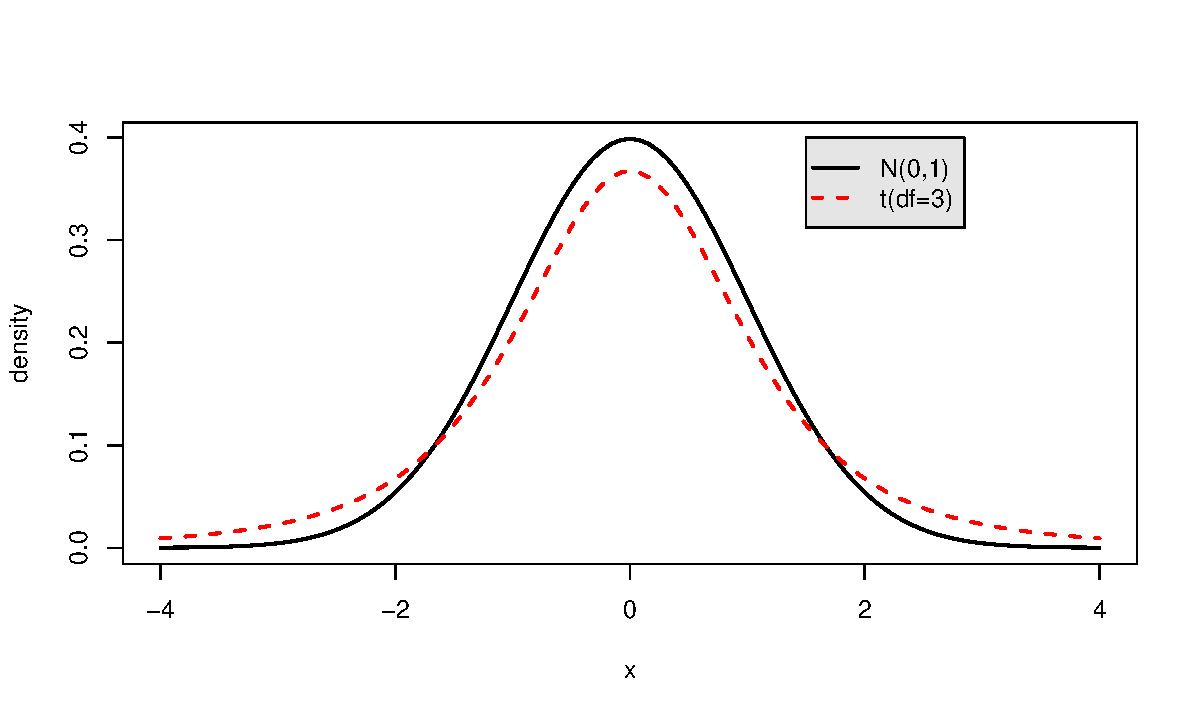
\includegraphics[width=1\linewidth]{figure/unnamed-chunk-13-1} 

}



\end{knitrout}
\end{frame}


\begin{frame}{What sample size needed?}

\begin{itemize}
	\setlength\itemsep{1em}
	\item The `balancing formula', in SEM terms, is simply the $n$ where
	$$ 1.645 \times SEM + 0.84 \times SEM = \Delta.$$
	Replacing each of the  SEMs (assumed equal, because we assumed the variability
	is approx. the same under both scenarios) by $\sigma/\sqrt{n}$,  i.e.,
	
	$$ 1.645 \times \sigma/\sqrt{n} + 0.84 \times \sigma/\sqrt{n} = \Delta.$$
	
	and solving for $n$, one gets
	
	$$  n = (1.645 + 0.84)^2  \times \bigg\{ \frac{\sigma}{\Delta} \bigg\}^2 = 
	(1.645 + 0.84)^2  \times \bigg\{ \frac{Noise}{Signal} \bigg\}^2 .$$
\end{itemize}

\end{frame}


\begin{frame}{What sample size needed?}
\begin{itemize}
		\setlength\itemsep{1em}
	\item Notice the structure of the formula. The \textit{first} component has to do
	with the operating characteristics or performance of the test, i.e.,
	the type I error probability $\alpha$ and the desired power (the complement of the type II error probability, $\beta$).
	
	\pause 
	
	\item The \textit{second} has to do	with the context in which it is applied, i..e, the size of the noise relative to the  signal. \pause 
	
	\item In our example, where the \underline{Noise-to-Signal Ratio} is $\frac{\sigma = 0.0080}{\Delta = 0.0054}$ = 1.48, so that its square is $1.48^2$ or approx 2.2,	and $(1.645 + 0.84)^2 = 2.485^2$ = approx 6.2,	$$  n = 6.2  \times 2.2  =  13.6, \textrm{approx, or, rounded up,  } n = \textbf{14}. $$
\end{itemize}
\end{frame}



\begin{frame}[fragile]{Code for null and alternative distribution plots}
\begin{knitrout}\scriptsize
\definecolor{shadecolor}{rgb}{0.969, 0.969, 0.969}\color{fgcolor}
\begin{alltt}
\hlkwd{source}\hlstd{(}\hlstr{"https://raw.githubusercontent.com/sahirbhatnagar/EPIB607/
master/assignments/a6/plot_null_alt.R"}\hlstd{)}

\hlstd{mu0} \hlkwb{<-} \hlopt{-}\hlnum{0.540} \hlcom{# mean under the null}
\hlstd{mha} \hlkwb{<-} \hlnum{0.99}\hlopt{*-}\hlnum{0.540} \hlcom{# mean under the alternative}
\hlstd{s} \hlkwb{<-} \hlnum{0.0080} \hlcom{# sample/population SD}
\hlstd{n} \hlkwb{<-} \hlnum{5} \hlcom{# sample size}
\hlstd{cutoff} \hlkwb{<-} \hlstd{mu0} \hlopt{+} \hlkwd{qnorm}\hlstd{(}\hlnum{0.95}\hlstd{)} \hlopt{*} \hlstd{s} \hlopt{/} \hlkwd{sqrt}\hlstd{(n)}

\hlkwd{power_plot}\hlstd{(}\hlkwc{n} \hlstd{= n,}
        \hlkwc{s} \hlstd{= s,}
        \hlkwc{mu0} \hlstd{= mu0,}
        \hlkwc{mha} \hlstd{= mha,}
        \hlkwc{cutoff} \hlstd{= cutoff,}
        \hlkwc{alternative} \hlstd{=} \hlstr{"greater"}\hlstd{,}
        \hlkwc{xlab} \hlstd{=} \hlstr{"Freezing point (degrees C)"}\hlstd{)}
\end{alltt}

\end{knitrout}
\end{frame}


\begin{frame}[fragile]{Code for power as a function of sample size and noise}
\begin{knitrout}\scriptsize
\definecolor{shadecolor}{rgb}{0.969, 0.969, 0.969}\color{fgcolor}
\begin{alltt}
\hlkwd{source}\hlstd{(}\hlstr{"https://raw.githubusercontent.com/sahirbhatnagar/EPIB607/
master/assignments/a6/plot_null_alt.R"}\hlstd{)}

\hlstd{pacman}\hlopt{::}\hlkwd{p_load}\hlstd{(manipulate)} \hlcom{# or library(manipulate)}

\hlstd{mu0} \hlkwb{<-} \hlopt{-}\hlnum{0.540} \hlcom{# mean under the null}
\hlstd{mha} \hlkwb{<-} \hlnum{0.99}\hlopt{*-}\hlnum{0.540} \hlcom{# mean under the alternative}
\hlstd{s} \hlkwb{<-} \hlnum{0.0080}
\hlstd{n} \hlkwb{<-} \hlnum{5}
\hlstd{cutoff} \hlkwb{<-} \hlstd{mu0} \hlopt{+} \hlkwd{qnorm}\hlstd{(}\hlnum{0.95}\hlstd{)} \hlopt{*} \hlstd{s} \hlopt{/} \hlkwd{sqrt}\hlstd{(n)}

\hlstd{manipulate}\hlopt{::}\hlkwd{manipulate}\hlstd{(}
\hlkwd{power_plot}\hlstd{(}\hlkwc{n} \hlstd{= sample_size,} \hlkwc{s} \hlstd{= sample_sd,}
        \hlkwc{mu0} \hlstd{= mu0,} \hlkwc{mha} \hlstd{= mha,}
        \hlkwc{cutoff} \hlstd{= cutoff,}
        \hlkwc{alternative} \hlstd{=} \hlstr{"greater"}\hlstd{,}
        \hlkwc{xlab} \hlstd{=} \hlstr{"Freezing point (degrees C)"}\hlstd{),}
        \hlkwc{sample_size} \hlstd{= manipulate}\hlopt{::}\hlkwd{slider}\hlstd{(}\hlnum{5}\hlstd{,} \hlnum{100}\hlstd{),}
        \hlkwc{sample_sd} \hlstd{= manipulate}\hlopt{::}\hlkwd{slider}\hlstd{(}\hlnum{0.001}\hlstd{,} \hlnum{0.01}\hlstd{,} \hlkwc{initial} \hlstd{=} \hlnum{0.008}\hlstd{))}
\end{alltt}

\end{knitrout}
\end{frame}


\begin{frame}{Interpreting p-values from statistical tests}
\begin{itemize}
	\small
	\setlength\itemsep{1em}
	\item In the milk example, an $n=5$ gives an SEM of	$\sigma/\sqrt{5}$ = 0.0080/2236 = 0.0036. So the cutoff for a 1 sided test with $\alpha$ = 0.05 is $1.645 \times 0.0036 = 0.0059$ above -0.5400,
	i.e,. at - 0.5341. 
	\item This is computed under the null (innocence) hypothesis, namely that what we are testing is pure milk, with no added water. \pause 
	\item The 1 sided alternative is that we are testing a `less than 100\%, more than 0\%' mix, where the
	mean is above (to right of) -0.540, i.e., on the (upper) 'added water' side of the null. 
	\item Formally, these two hypotheses are 
	$$\textrm{H}_0: \mu = -0.540; \  H_{alt}: \mu > -0.540.$$
	\pause 
	\item Since the mean of the 5 measurements, namely -0.533$^{\circ}$C, is to the right of (\textbf{exceeds}) this threshold, it would be considered `statistically significant at the 0.05 level.' The actual p-value is \texttt{pnorm(-0.533, mean=-0.54, sd = 0.0036, lower.tail=FALSE)} = \underline{0.026}.
\end{itemize}
\end{frame}

\begin{frame}{Is this good evidence that the producer is adding water to the milk?}
\begin{itemize}
	\small
	\setlength\itemsep{1em}
	\pause 
	\item Do  not jump to conclusions and immediately accuse the supplier of cheating
	\pause 
	\item In particular, it would not be appropriate -- or accurate -- to say that you are 1 - 0.026 = 0.974 = 97.4\% certain that the supplier is cheating. 
	\item Remember that a \underline{p-value} is a probability \underline{concerning the data}, \textbf{conditional} on (i.e., computed	under the  assumption that) H$_0$  being (is) true.  In other words, the p-value has to do with P(data $|$ `innocence'), whereas at issue is the reverse,  P(`innocence' $|$ data).
	\pause 
	\item As to this latter probability (of being innocent), there are a lot of other factors to consider first, before accusing the supplier of cheating.
\end{itemize}
\end{frame}


\begin{frame}{Other factors to consider before accusing the supplier}
\begin{itemize}
	\small
	\setlength\itemsep{1em}
	\item First, did you (re-)check the calculations?  How recently was the instrument 
	calibrated? etc. \pause 
	\item JH calls these \textbf{Type III errors}: the data were wrong, or the
		instrument was wrong, or the technician mis-calculated something. 
	\item It should remind us that, in the \textit{real} world, there are \textit{many} alternative hypotheses, not just the one.
	\pause 
	\item Second, why did you chose to test \textbf{this} supplier? \pause
	\begin{itemize}
		\item Is it someone that the manager suspected based on previous data, or based on knowing that he is behind in his loan payments to the bank? 
		\item Or maybe the laboratory manager merely asked a technician to start randomly testing, and the first supplier (blindly) chosen was the manager's brother-in-law?
	\end{itemize}
\end{itemize}
\end{frame}



\begin{frame}{Are all $p$-values created equal?}
\begin{itemize}
	\small
	\setlength\itemsep{1em}
	\item So, you can see that, just as in medical tests, there are\textbf{ many other pieces of evidence} or information, or circumstances, besides the $p$-value, that bear on the probability of innocence or guilt.
	\item This is very nicely brought out in the article `Are all p-values created equal?' which you can
	here: { \footnotesize \url{http://www.biostat.mcgill.ca/hanley/BionanoWorkshop/AreAllSigPValuesCreatedEqual.pdf}}
	
	\item Sadly, the mixing up of P(data $|$ hypothesis) and P(data $|$ data) -- often referred to as
	`The Prosecutor's Fallacy' -- is  common, and can lead to serious harm. 
\end{itemize}
\end{frame}


\begin{frame}{When does the $p$-value work well?}
\begin{itemize}
	\small
	\setlength\itemsep{1em}
	\item The use of $p$-values works well in \underline{Quality Control}, where the aim is to detect
	(the \underline{few})  deviations ('\underline{bad}' ones)  from the desired specifications, to stop and fix	the offending machine, or to flag defective batches. \pause 
	\item It is not clear that it is equally effective at identifying the (\underline{few}) truly active (`{good}) compounds	via the mass testing of lots of compounds, most of which are expected to be inactive -- and then investing all one's effort in these few `good' ones at the next stage of development.
\end{itemize}
\end{frame}


\section{Another example on power: Lake Wobegon}

\begin{frame}[fragile]{Power: Lake Wobegon}
\small
\begin{itemize}
	\item It is claimed that the children of Lake Wobegon are above
	average. Take a simple random sample of 9 children from Lake
	Wobegon, and measure their IQ to obtain a sample mean of 112.8. 
	\item IQ scores are scaled to be Normally distributed with mean 100 and
	standard deviation 15. 
	\item Does this sample provide evidence to reject the null hypothesis of no difference between children of Lake Wobegon and the general population? \pause 
	\item[]\item[1.] \textcolor{blue}{Null and alternative hypotheses:} The claim made is
	that the population of children Lake Wobegon have higher than
	average intellidence. Thus the null hypothesis is that the
	population has average intelligence, or a score of 100. Therefore
	$H_0: \mu=100$, and the (one-sided) alternative is $H_A: \mu >
	100$.
\end{itemize}
\end{frame}


\begin{frame}[fragile]{Lower limit of 95\% CI}
\small
	\begin{enumerate}
		\item \underline{Hypotheses.} $H_0: \mu = 100$, $H_A: \mu > 100$.
		\item \underline{Calculate 95\% CI.}
\begin{knitrout}\scriptsize
\definecolor{shadecolor}{rgb}{0.969, 0.969, 0.969}\color{fgcolor}
\begin{alltt}
\hlstd{mosaic}\hlopt{::}\hlkwd{xqnorm}\hlstd{(}\hlkwc{p} \hlstd{=} \hlkwd{c}\hlstd{(}\hlnum{0.05}\hlstd{,}\hlnum{1}\hlstd{),} \hlnum{112.8}\hlstd{,} \hlnum{15}\hlopt{/}\hlkwd{sqrt}\hlstd{(}\hlnum{9}\hlstd{))}
\end{alltt}


{\centering 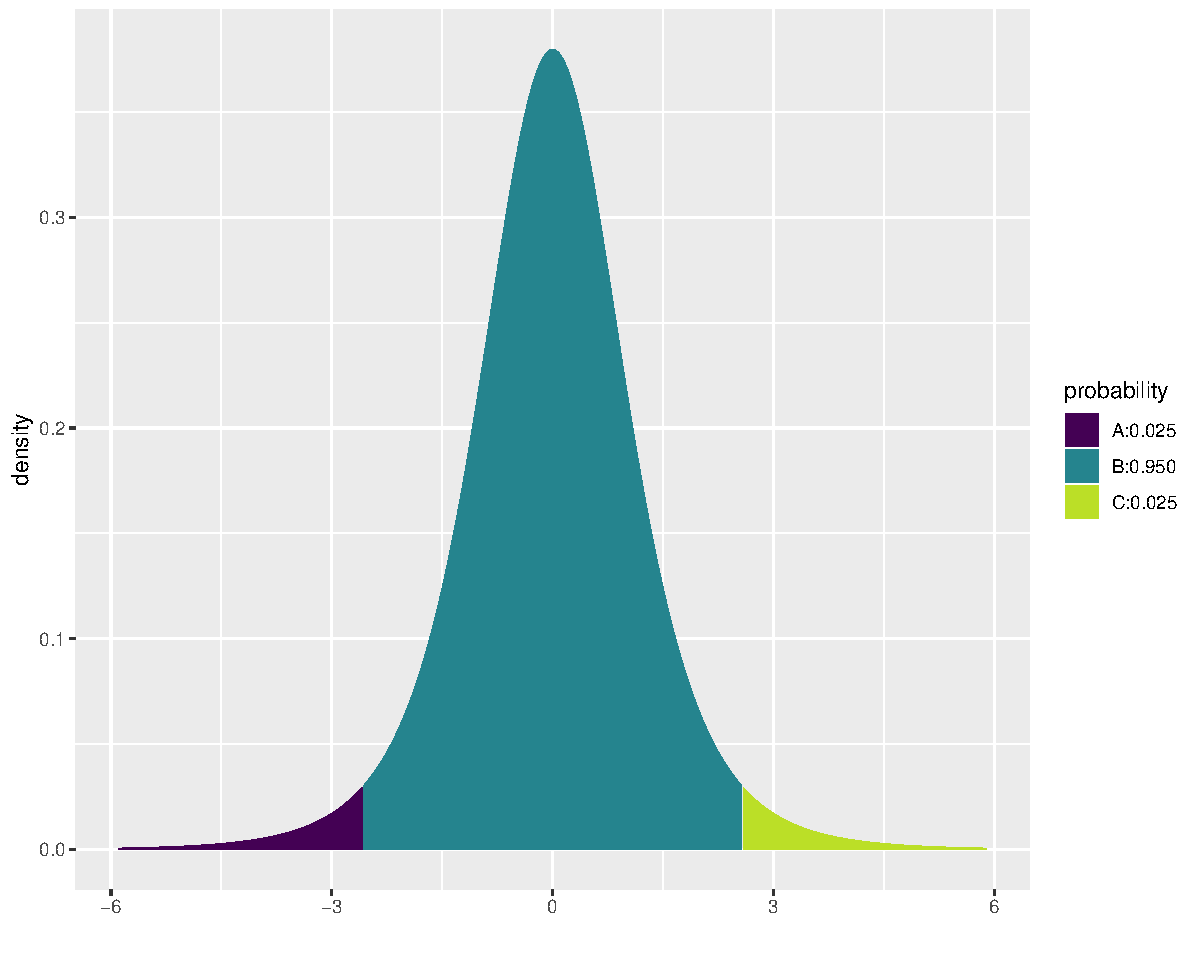
\includegraphics[width=1\linewidth]{figure/unnamed-chunk-16-1} 

}


\begin{verbatim}
## [1] 104.5757      Inf
\end{verbatim}

\end{knitrout}
\pause 
\item \underline{Statement.} The lower limit of the CI excludes $\mu_0=100$, and so \underline{there is evidence to suggest} that the children at Lake Wobegon are brighter than other children at the $\alpha=0.05$ level.
	\end{enumerate}

\end{frame}

\frame{\frametitle{Power} Steps to finding power:
	\begin{enumerate}
		\item State null hypothesis, $H_0$, and state a specific alternative, $H_A$, as the minimum (clinical/substantive) departure from the null hypothesis that would
		be of interest. \pause
		\item Find the values of $\overline{y}$ that lead to rejection of
		$H_0$. \pause
		\item Calculate the probability of observing the values found in
		(2) when the alternative is true.
	\end{enumerate}
} \frame{\frametitle{Power} Example: Lake Wobegon\\
	Suppose you hope to use a \textbf{one-sided} test to show that the children from Lake
	Wobegon are at least 10 points higher than average on the IQ test. What power do you have
	to detect this with the sample of 9 children if using a 0.05-level test? \\ \ \\ \pause
	\begin{enumerate}
		\item \underline{Hypotheses.} $H_0: \mu = 100$, $H_A: \mu > 110$. \pause
		\item[] \item \underline{Find values of the sample mean that reject the
			null.}\\ \ \\ The test will reject $H_0$ at the 0.05 level whenever
		\[z = \frac{\overline{y}-\mu_0}{\sigma/\sqrt{n}} =
		\frac{\overline{y}-100}{15/\sqrt{9}} \ge 1.645.\] Now we must
		translate this back to values of $\overline{y}$...
	\end{enumerate}
} \frame{\frametitle{Power} Example: Lake Wobegon\\
	\begin{enumerate}
		\item[2.] \underline{Values of the sample mean that reject $H_0$
			(con't)}\\ \ \\
		The test will reject $H_0$ at the 0.05 level whenever \[
		\frac{\overline{y}-100}{15/\sqrt{9}} \ge 1.645,\] which means we
		reject $H_0$ whenever \[ \overline{y} \ge 1.645\times 15/\sqrt{9}+100 = 108.2\]
		If $H_0$ is true, the probability of seeing an IQ score as big as
		108.2 or bigger is 5\%.
	\end{enumerate}
} \frame{\frametitle{Power} Example: Lake Wobegon\\
	\begin{enumerate}
		\item[3.] \underline{Find the probability of rejecting $H_0$ if
			$\mu=\mu_A=110$.}\\ \ \\
		$P(\overline{y} > 108.2|\mu=\mu_A=110) $
		\begin{eqnarray*} \qquad \qquad & = &
			P\left(\left.\frac{\overline{y}-\mu_A}{\sigma/\sqrt{n}}
			> \frac{108.2-110}{15/\sqrt{9}}\right|\mu=\mu_A=110\right)\\
			& = & P\left(z > -0.36\right)\\
			& = & 0.64\\
		\end{eqnarray*}
		So there is approximately a 2/3 chance of detecting a difference of
		10 points on the IQ scale at the 0.05 level of significance with a
		sample size of 9.
	\end{enumerate}
} 


\begin{frame}[fragile]{Null and alternative distribution plots}
\begin{knitrout}\scriptsize
\definecolor{shadecolor}{rgb}{0.969, 0.969, 0.969}\color{fgcolor}
\begin{alltt}
\hlkwd{power_plot}\hlstd{(}\hlkwc{n} \hlstd{=} \hlnum{9}\hlstd{,} \hlkwc{s} \hlstd{=} \hlnum{15}\hlstd{,} \hlkwc{mu0} \hlstd{=} \hlnum{100}\hlstd{,} \hlkwc{mha} \hlstd{=} \hlnum{110}\hlstd{,}
        \hlkwc{cutoff} \hlstd{=} \hlnum{100} \hlopt{+} \hlkwd{qnorm}\hlstd{(}\hlnum{0.95}\hlstd{)} \hlopt{*} \hlnum{15} \hlopt{/} \hlkwd{sqrt}\hlstd{(}\hlnum{9}\hlstd{),}
        \hlkwc{alternative} \hlstd{=} \hlstr{"greater"}\hlstd{,} \hlkwc{xlab} \hlstd{=} \hlstr{"Average IQ Score"}\hlstd{)}
\end{alltt}


{\centering 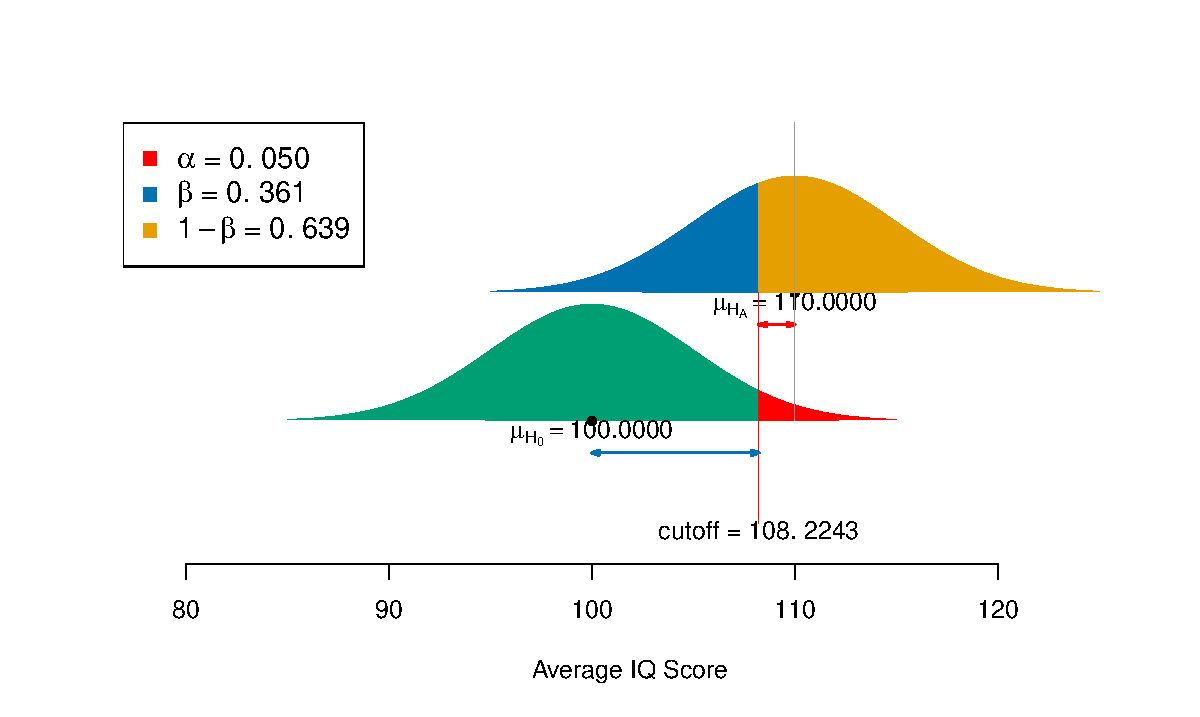
\includegraphics[width=1\linewidth]{figure/unnamed-chunk-17-1} 

}



\end{knitrout}
\end{frame}



\frame{\frametitle{Power} Example: Lake Wobegon\\ \ \\
	If you hoped to use a \underline{two-sided test} to show that the children from Lake Wobegon are at
	least 10 points higher than average on the IQ test, what power do you have with the
	sample size of 9 and a 0.05-level test? \pause
	\begin{enumerate}
		\item \underline{Hypotheses.} $H_0: \mu = 100$, $H_A: \mu = 110$.\pause 
		\item[] \item \underline{Find values of the sample mean that reject the
			null.}\\ \ \\ The test will reject $H_0$ at the 0.05 level whenever
		\[z = \frac{\overline{y}-\mu_0}{\sigma/\sqrt{n}} =
		\frac{\overline{y}-100}{15/\sqrt{9}} \ge \textcolor{red}{1.96}
		\qquad \hbox{\textbf{\textcolor{blue}{OR when}}}\]
		\[z = \frac{\overline{y}-\mu_0}{\sigma/\sqrt{n}} =
		\frac{\overline{y}-100}{15/\sqrt{9}} \le \textcolor{red}{-1.96}\]
		since we are performing a two-sided test.
	\end{enumerate}
} \frame{\frametitle{Power} Thus we reject $H_0$ if $\overline{y}
	\ge 1.96\times5+100 = 109.8$ \textbf{OR} if $\overline{y} \le
	-1.96\times5+100 = 90.2$
	\begin{enumerate}
		\item[3.] \underline{Find the probability of rejecting $H_0$ if
			$\mu=\mu_A=110$.}\\ \ \\
		$P(\overline{y} > 109.8 \hbox{\textbf{ OR }} \overline{y} <
		90.2|\mu=\mu_A=110) $
		\begin{eqnarray*} \qquad & = & P(\overline{y} >
			109.8|\mu_A=110) + P(\overline{y} < 90.2|\mu_A=110)\\
			& = & P\left(\left.\frac{\overline{y}-\mu_A}{\sigma/\sqrt{n}}
			> \frac{109.8-110}{15/\sqrt{9}}\right|\mu_A=110\right)\\
			&  & \quad + P\left(\left.\frac{\overline{y}-\mu_A}{\sigma/\sqrt{n}}
			< \frac{90.2-110}{15/\sqrt{9}}\right|\mu_A=110\right)\\
			& = & P\left(z > -0.04\right) + P\left(z < -3.96\right)\\
			& = & 0.52 + 3.7\times10^{-5} \approx 0.52\\
		\end{eqnarray*}
		There is about a 1/2 chance of detecting a difference of 10 pts on
		the IQ scale at the 0.05 level of significance with $n=9$ using a
		two-sided alternative hypothesis.
	\end{enumerate}
} \frame{\frametitle{Power} 
\small 

\begin{itemize}
	\item Steps 1 and 2 used to find the power of a one-sided test to detect a difference of $x$ points above (or below) the population mean are similar to the steps for finding the power of a two-sided test to detect a difference of $x$ points on either side of the population mean. 
	\item However for a two-sided test, there will be two sets of values of $\overline{y}$
		that lead us to reject $H_0$ (also, $z_\alpha$ for one-sided and
		$z_{\alpha/2}$ for two-sided).  %\pause
		
		\item \textbf{However}, there is one critical difference in the third step: we need to
		calculate the probability of seeing $\overline{y}$ in either of the two tails (rejection
		regions) of the null distribution under the assumption that the true distribution has
		mean $\mu_A$. So there will be two probabilities to calculate in the third step. 
		\pause
		
		\item Note: If we felt that the minimum significant departure from $\mu_0$
		was different above and below (e.g., we are interested in increases
		of blood pressure of at least 3.5mmHg and decreases of blood
		pressure of at least 2mmHg), we perform the calculations as though
		we were interested in the minimum of the two values (Why?).
\end{itemize}
 } 

\frame{\frametitle{Power} Exercises: Lake Wobegon\\ \ \\
	Find the power of the following tests, assuming two-sided
	alternative hypotheses:
	\begin{enumerate}
		\item A 0.05-level test to detect a difference of 15 points on the
		IQ scale using the 9 children.
		\item A 0.05-level test to detect a difference of 5 points on the
		IQ scale using the 9 children.
		\item A 0.05-level test to detect a difference of 10 points on the
		IQ scale using 25 children.
		\item A 0.01-level test to detect a difference of 10 points on the
		IQ scale using the 9 children.
\end{enumerate} }

\end{document}



























\begin{frame}[fragile]{$t_{(5)}$ distribution vs. Standard Normal distribution}
\begin{minipage}{0.47\textwidth}
\begin{knitrout}\scriptsize
\definecolor{shadecolor}{rgb}{0.969, 0.969, 0.969}\color{fgcolor}
\begin{alltt}
\hlkwd{library}\hlstd{(mosaic)}
\hlkwd{xqnorm}\hlstd{(}\hlkwc{p} \hlstd{=} \hlkwd{c}\hlstd{(}\hlnum{0.025}\hlstd{,} \hlnum{0.975}\hlstd{))}
\end{alltt}

\end{knitrout}
\begin{knitrout}\scriptsize
\definecolor{shadecolor}{rgb}{0.969, 0.969, 0.969}\color{fgcolor}

{\centering 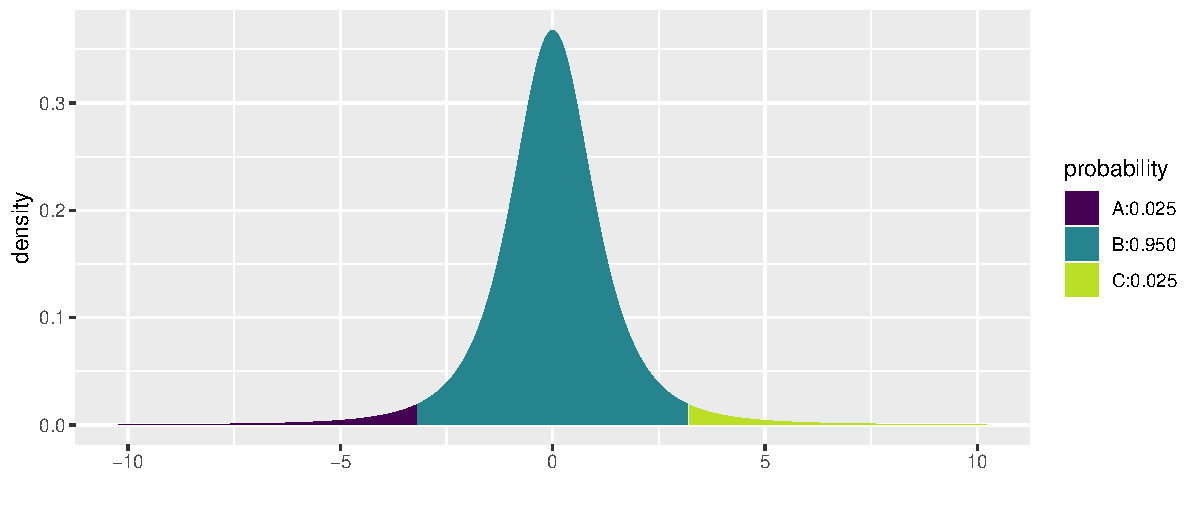
\includegraphics[width=1\linewidth]{figure/unnamed-chunk-19-1} 

}


\begin{verbatim}
## [1] -1.959964  1.959964
\end{verbatim}

\end{knitrout}
\end{minipage}
\begin{minipage}{0.5\textwidth}
\begin{knitrout}\scriptsize
\definecolor{shadecolor}{rgb}{0.969, 0.969, 0.969}\color{fgcolor}
\begin{alltt}
\hlkwd{library}\hlstd{(mosaic)}
\hlkwd{xqt}\hlstd{(}\hlkwc{p} \hlstd{=} \hlkwd{c}\hlstd{(}\hlnum{0.025}\hlstd{,} \hlnum{0.975}\hlstd{),} \hlkwc{df} \hlstd{=} \hlnum{5}\hlstd{)}
\end{alltt}


{\centering 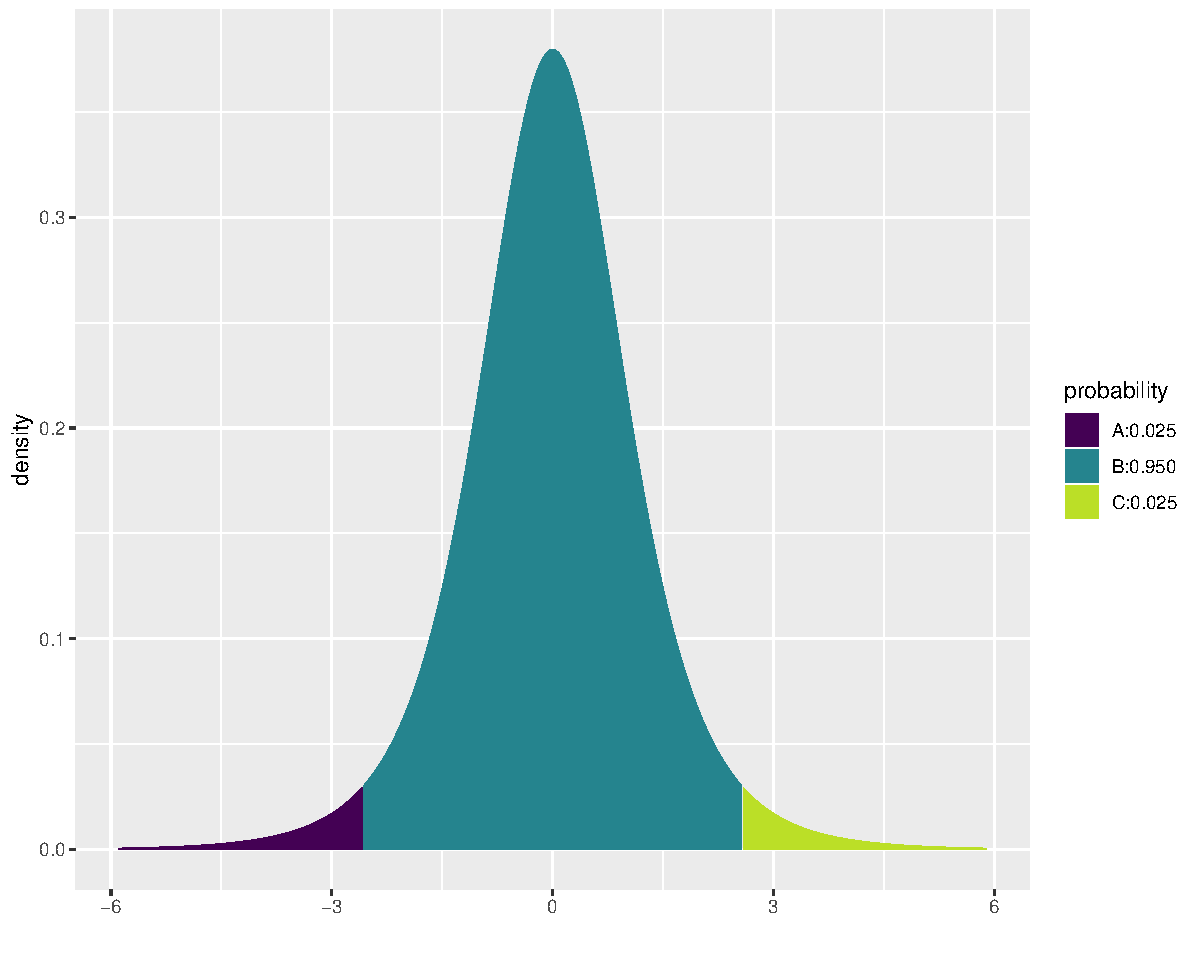
\includegraphics[width=1\linewidth]{figure/unnamed-chunk-20-1} 

}


\begin{verbatim}
## [1] -2.570582  2.570582
\end{verbatim}

\end{knitrout}
\end{minipage}
\end{frame}




\begin{frame}[fragile]{$t_{(30)}$ distribution vs. Standard Normal distribution}
\begin{minipage}{0.47\textwidth}
\begin{knitrout}\scriptsize
\definecolor{shadecolor}{rgb}{0.969, 0.969, 0.969}\color{fgcolor}
\begin{alltt}
\hlkwd{library}\hlstd{(mosaic)}
\hlkwd{xqnorm}\hlstd{(}\hlkwc{p} \hlstd{=} \hlkwd{c}\hlstd{(}\hlnum{0.025}\hlstd{,} \hlnum{0.975}\hlstd{))}
\end{alltt}

\end{knitrout}
\begin{knitrout}\scriptsize
\definecolor{shadecolor}{rgb}{0.969, 0.969, 0.969}\color{fgcolor}

{\centering 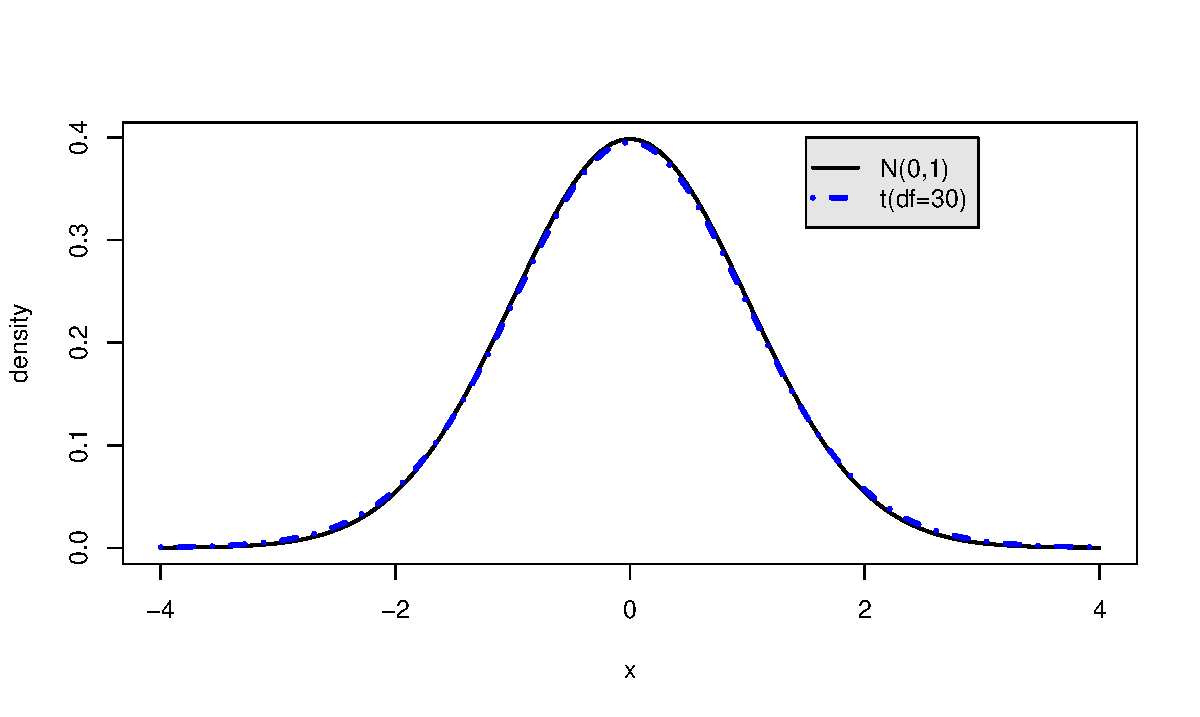
\includegraphics[width=1\linewidth]{figure/unnamed-chunk-22-1} 

}


\begin{verbatim}
## [1] -1.959964  1.959964
\end{verbatim}

\end{knitrout}
\end{minipage}
\begin{minipage}{0.5\textwidth}
\begin{knitrout}\scriptsize
\definecolor{shadecolor}{rgb}{0.969, 0.969, 0.969}\color{fgcolor}
\begin{alltt}
\hlkwd{library}\hlstd{(mosaic)}
\hlkwd{xqt}\hlstd{(}\hlkwc{p} \hlstd{=} \hlkwd{c}\hlstd{(}\hlnum{0.025}\hlstd{,} \hlnum{0.975}\hlstd{),} \hlkwc{df} \hlstd{=} \hlnum{30}\hlstd{)}
\end{alltt}

\end{knitrout}
\begin{knitrout}\scriptsize
\definecolor{shadecolor}{rgb}{0.969, 0.969, 0.969}\color{fgcolor}

{\centering 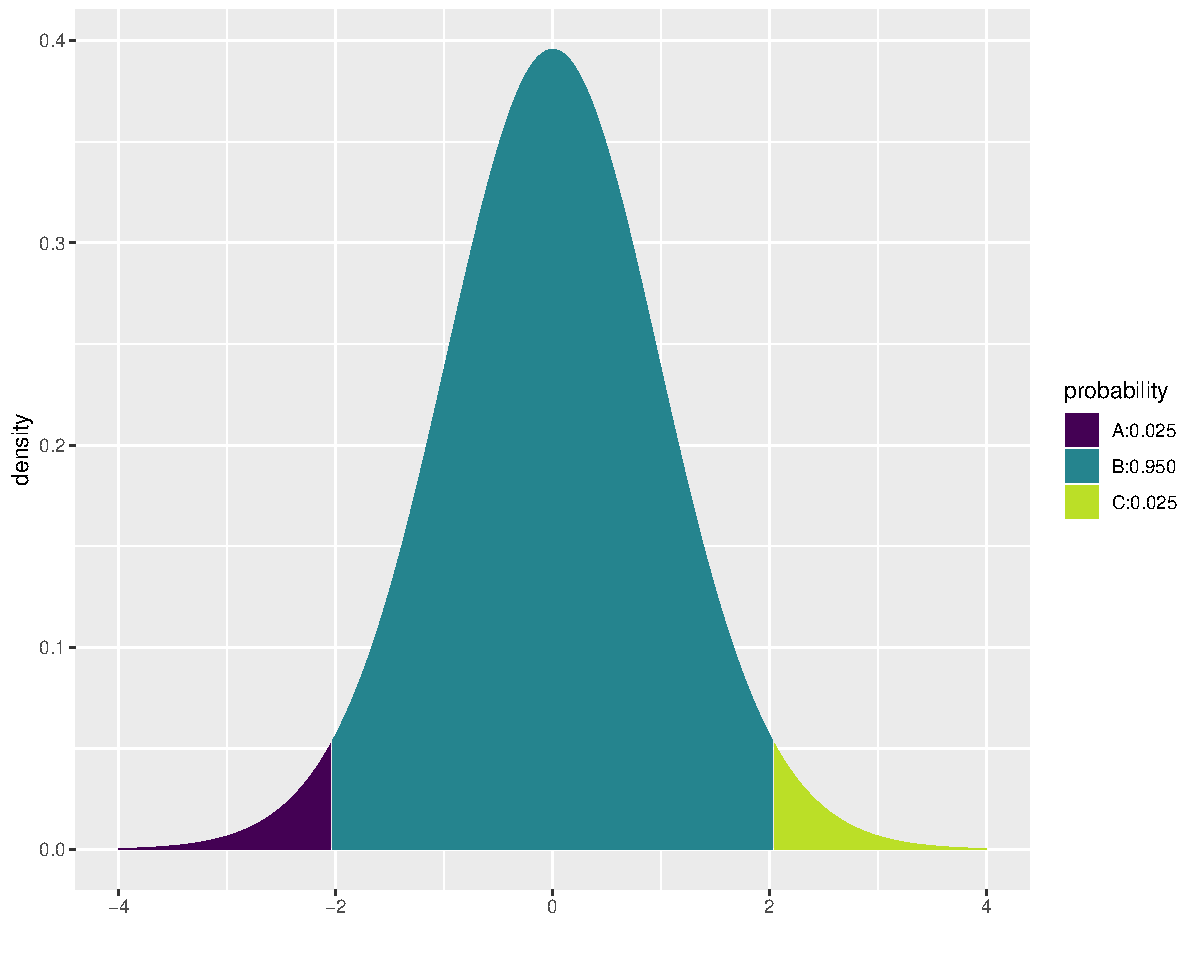
\includegraphics[width=1\linewidth]{figure/unnamed-chunk-24-1} 

}


\begin{verbatim}
## [1] -2.042272  2.042272
\end{verbatim}

\end{knitrout}
\end{minipage}
\end{frame}

%\frame{\frametitle{$t$ distributions}
%	\begin{figure}
%		\begin{center}
%			\epsfig{figure=Tables/psls_table_C.eps,scale=.35}
%		\end{center}
%	\end{figure}
%}


\begin{frame}{$t$ distributions}
\begin{itemize}
	\small
	\item Is symmetric around 0 ( just like the $\mathcal{N}(0,1)$ )
	\item Has a shape like that of the Z distribution, but with a SD slightly larger than
	unity i.e. slightly flatter and heavier-tailed
	\item Shape becomes indistinguishable from Z distribution as $n \rightarrow \infty$ (in fact as $n$ goes much beyond 30)
	\item Instead of  $\pm 1.96 \times  $ SEM for 95\% confidence (or to use as the critical value in a null-hypothesis test), we need these multiples (or critical values): \\ \ \\
	
	\begin{tabular}{r r r r}
		$n$ & `degrees of freedom' & Multiple & from \texttt{R} \\ 
		\hline
		2 & 1 & 12.71 & \texttt{qt(0.975,  1)} \\
		3 & 2 & 4.30 & \texttt{qt(0.975,  2)}\\
		4 & 3 & 3.18 & \texttt{qt(0.975,  3)}\\
		11 &10 & 2.23 & \texttt{qt(0.975, 10)}  \\
		21 & 20 & 2.09 & \texttt{qt(0.975, 20)} \\
		31 & 30 & 2.04 & \texttt{qt(0.975, 30)} \\
		121 & 120 & 1.98 & \texttt{qt(0.975,120)} \\
		$\infty$ & $\infty$ & 1.96 & \texttt{qt(0.975,Inf)}   \\
	\end{tabular}
	
\end{itemize}
\end{frame}

 

\begin{frame}[fragile]{$t$ distributions}
Sample size increases $\rightarrow$ degrees of freedom increase $\rightarrow$ $t$ starts to look like $\mathcal{N}(0,1)$
\begin{knitrout}\scriptsize
\definecolor{shadecolor}{rgb}{0.969, 0.969, 0.969}\color{fgcolor}

{\centering 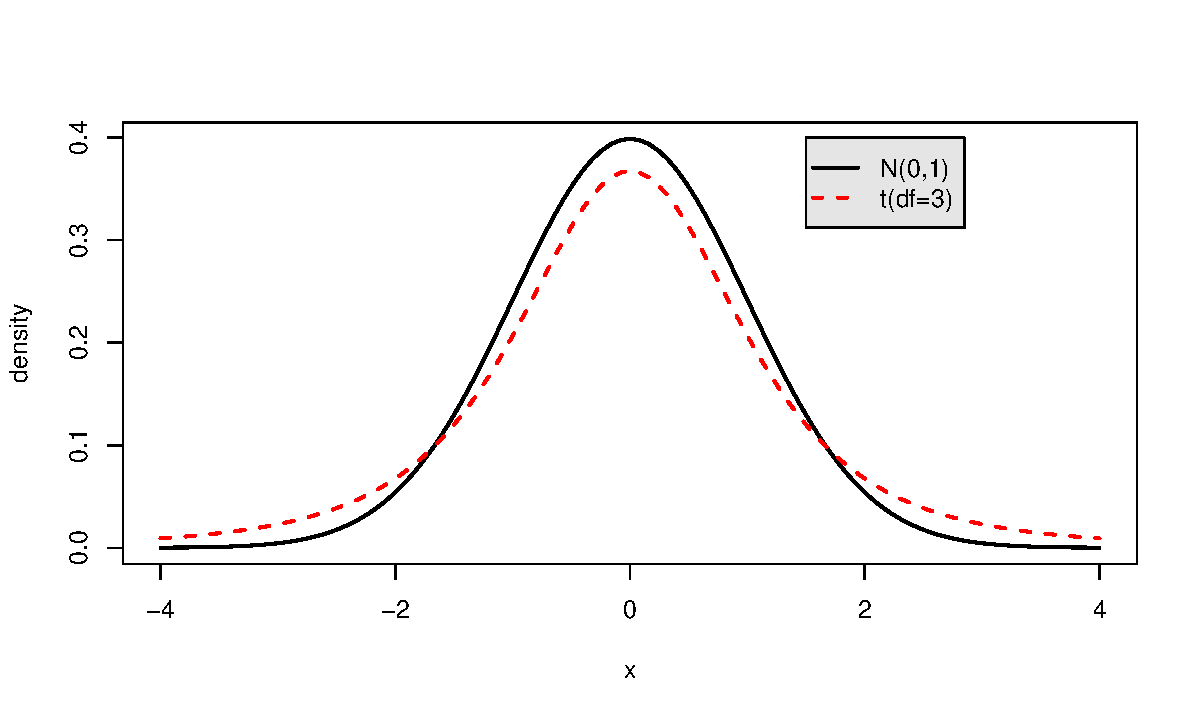
\includegraphics[width=1\linewidth]{figure/unnamed-chunk-25-1} 

}



\end{knitrout}
\end{frame}

\begin{frame}[fragile]{$t$ distributions}
Sample size increases $\rightarrow$ degrees of freedom increase $\rightarrow$ $t$ starts to look like $\mathcal{N}(0,1)$
\begin{knitrout}\scriptsize
\definecolor{shadecolor}{rgb}{0.969, 0.969, 0.969}\color{fgcolor}

{\centering 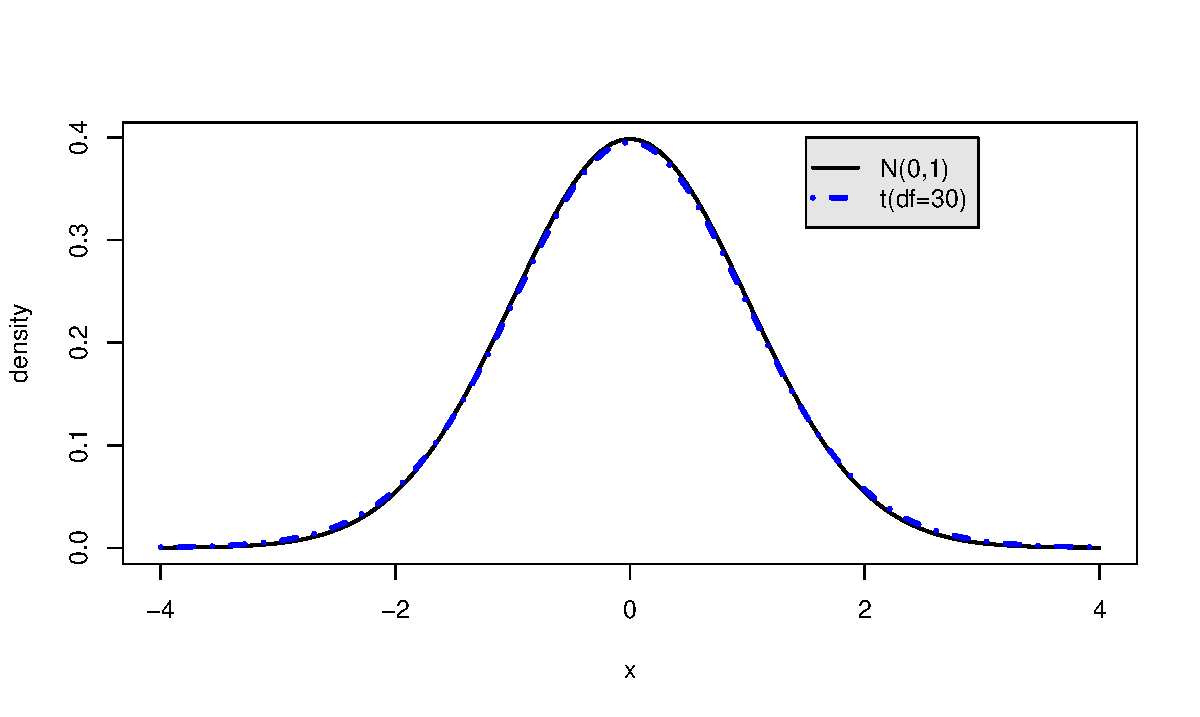
\includegraphics[width=1\linewidth]{figure/unnamed-chunk-26-1} 

}



\end{knitrout}

\Large This is where the infamous $n=30$ comes from !!
\end{frame}

\frame{\frametitle{$t$ procedures} We can calculate CIs and
	perform significance tests much as before (example coming up
	soon).\\\ \\
	
	A significance test of a single sample mean using the $t$-statistic
	is called a \textcolor{blue}{one-sample $t$-test}. \\ \ \\
	
	Collectively, the significance tests and confidence-interval based
	tests using the $t$ distribution are called \underline{$t$ procedures}.  \\ \ \\
	
}

\begin{frame}{The one-sample $t$ test}

\Wider[4em]{
	\centering
		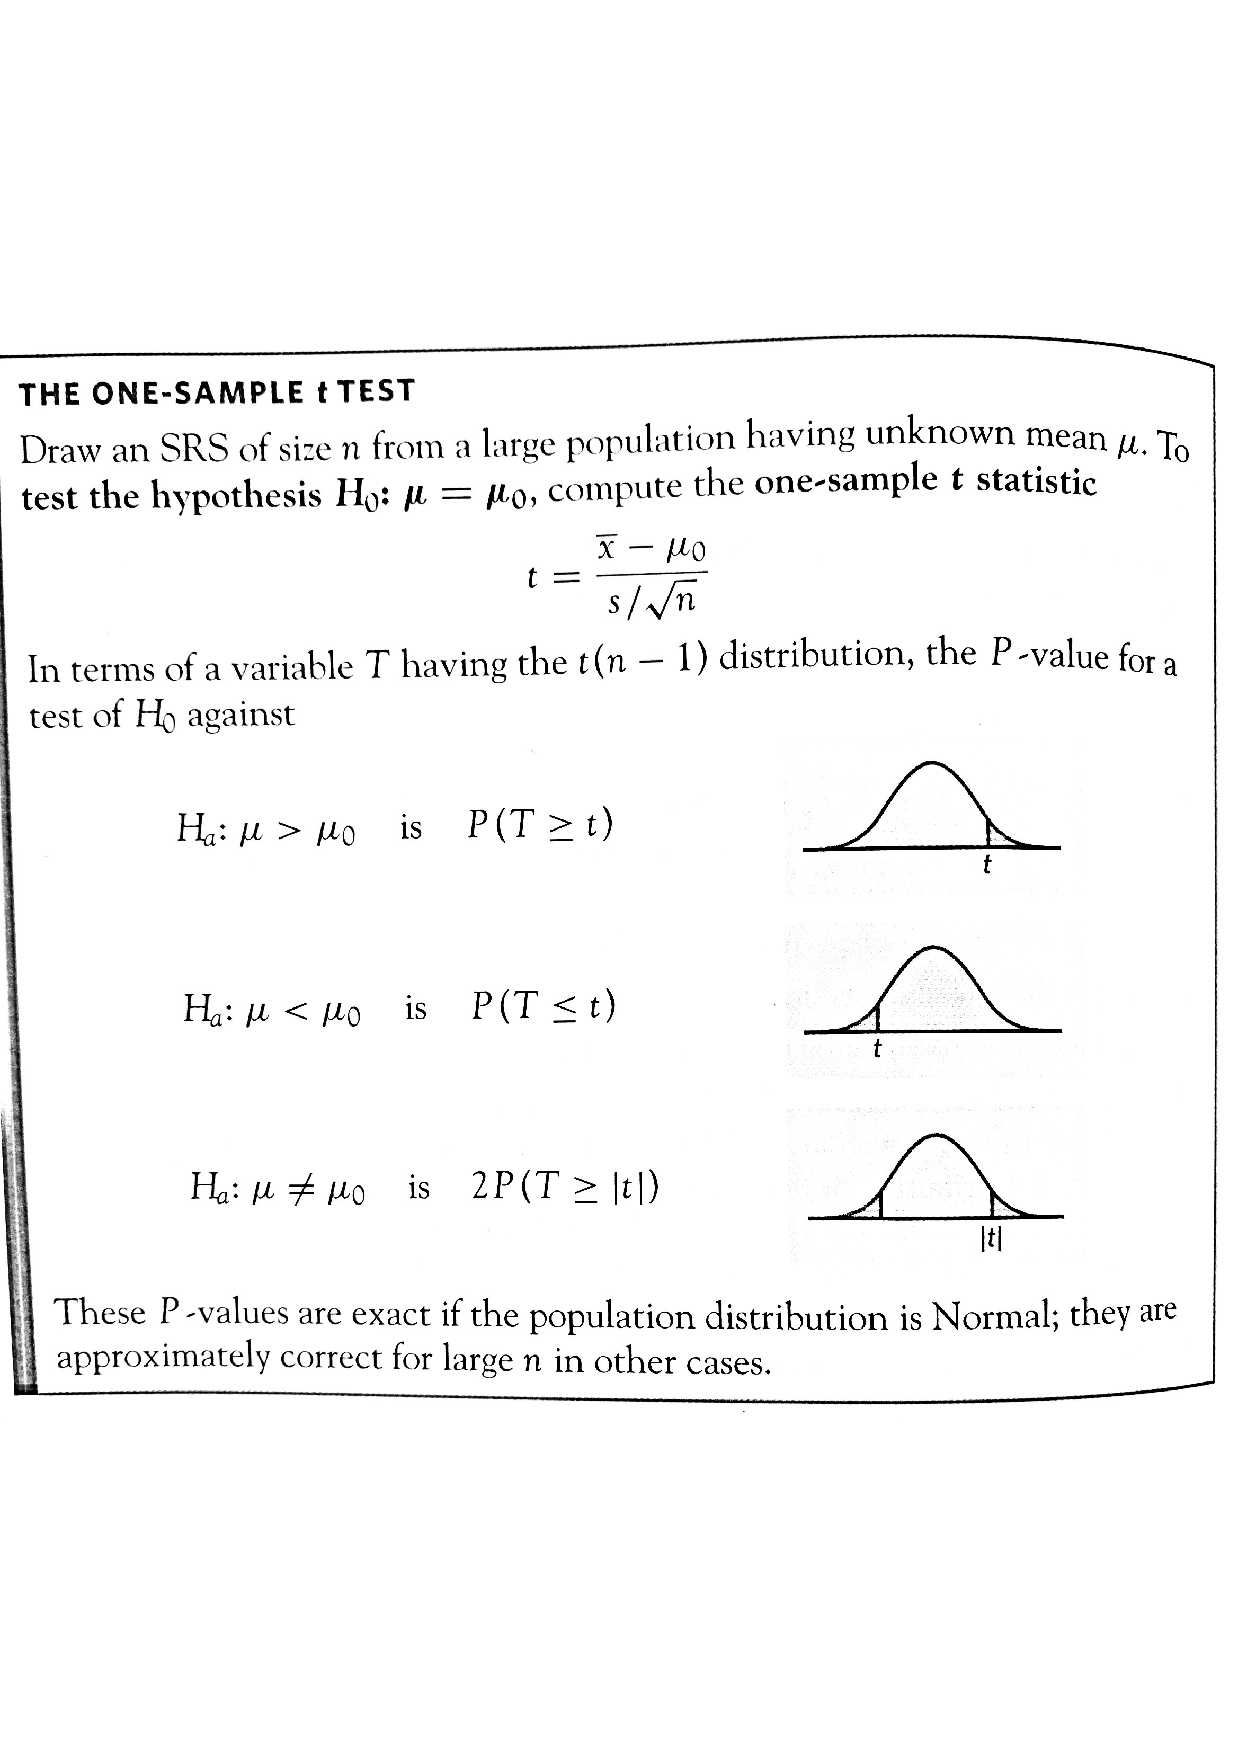
\includegraphics[scale=0.35]{ttest.pdf}
	
}

\end{frame}

 
\begin{frame}{A note about the conditions for $t$ procedures}

\begin{itemize}
	\setlength\itemsep{1em}
	\item B\&M stress that the \textbf{first} of their conditions as \textit{very important}: \textit{we can regard} our data as a simple random sample (SRS) from  the population \pause 
	\item The \textbf{second}, observations from the population have a \textit{\underline{Normal}} distribution with unknown mean parameter $\mu$ and unknown standard deviation parameter $\sigma$ less so 
	\item \textit{In practice}, inference procedures \textit{can accommodate some deviations from
		the Normality condition} when the sample is large enough. 
\end{itemize}
\end{frame}


\frame{\frametitle{Robustness of the $t$ procedures} A statistical
	procedure is said to be \textbf{robust} if it is insensitive to
	violations of the assumptions made. \\ \ \\
	\begin{itemize}
			\setlength\itemsep{1em}
		%\item Results of $t$ procedures (CIs, significance tests) are exact if the
		%population from which the simple random sample was drawn is Normal. \pause
		\item $t$ procedures are not robust against \textit{extreme}
		skewness, \underline{in small samples}, since the procedures are
		based on using $\overline{y}$ and $s$ (which are sensitive to
		outliers).
		\item Recall: \textcolor{blue}{Unless there is a very compelling reason
			(e.g.~known/confirmed error in the recorded data), outliers should not be discarded.}
		
	\end{itemize}
} \frame{\frametitle{Robustness of the $t$ procedures}
	\begin{itemize}
					\setlength\itemsep{2em}
		\item $t$ procedures \textbf{are} robust against other forms
		of non-normality and, even with considerable skew, perform well when $n$ is large. Why?
		\pause
		\item When $n$ is large, $s$ is a good estimate of $\sigma$
		(recall that $s$ is unbiased and, like most estimates, precision
		improves with increasing sample size) \pause
		\item CLT: $\overline{y}$ will be Normal when $n$ is large, even if the
		population data are not


	\end{itemize}
}



\begin{frame}{When and why we use the $t$-distribution}
\mylist{When $\sigma$ is unknown use $t$ distribution. \blue{but why?}; \pause the spread of the $t$ distribution is greater than $\mathcal{N}(0,1)$  }
\end{frame}



\begin{frame}[fragile]{Rejecting the Null ($H_0: \mu = \mu_0$) when $\sigma$ is known}
\small
\[ \underbrace{z_{0.975}}_{\textrm{critical value}}=1.96 = \frac{\bar{y}-\mu_0}{\sigma/\sqrt{n}} \rightarrow \frac{1.96 }{\sqrt{n}}\sigma = \bar{y}-\mu_0   \] which means that to reject $H_0$ the difference between your sample mean and $\mu_0$ needs to be \blue{greater than $\frac{1.96}{\sqrt{n}}$ standard deviations} 

\begin{knitrout}\scriptsize
\definecolor{shadecolor}{rgb}{0.969, 0.969, 0.969}\color{fgcolor}
\begin{alltt}
\hlstd{mosaic}\hlopt{::}\hlkwd{xqnorm}\hlstd{(}\hlkwc{p} \hlstd{=} \hlkwd{c}\hlstd{(}\hlnum{0.025}\hlstd{,} \hlnum{0.975}\hlstd{))}
\end{alltt}


{\centering 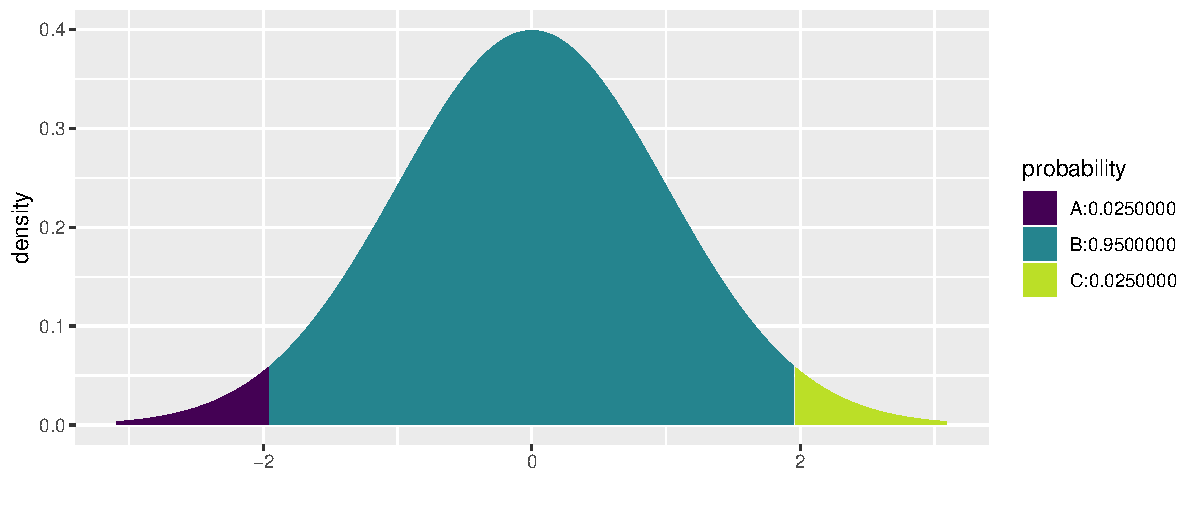
\includegraphics[width=1\linewidth]{figure/unnamed-chunk-28-1} 

}


\begin{verbatim}
## [1] -1.959964  1.959964
\end{verbatim}

\end{knitrout}
\end{frame}



\begin{frame}[fragile]{Rejecting the Null ($H_0: \mu = \mu_0$) when $\sigma$ is unknown}
\small
\[ \underbrace{t_{0.975,df=3}^\star}_{\textrm{critical value}}=3.18 = \frac{\bar{y}-\mu_0}{s/\sqrt{n}} \rightarrow  \frac{3.18}{\sqrt{n}}s = \bar{y}-\mu_0   \] which means that to reject $H_0$ the difference between your sample mean and $\mu_0$ needs to be \blue{greater than $\frac{3.18}{\sqrt{n}}$ standard deviations} 


\begin{knitrout}\scriptsize
\definecolor{shadecolor}{rgb}{0.969, 0.969, 0.969}\color{fgcolor}
\begin{alltt}
\hlstd{mosaic}\hlopt{::}\hlkwd{xqt}\hlstd{(}\hlkwc{p} \hlstd{=} \hlkwd{c}\hlstd{(}\hlnum{0.025}\hlstd{,} \hlnum{0.975}\hlstd{),} \hlkwc{df} \hlstd{=} \hlnum{3}\hlstd{)}
\end{alltt}


{\centering 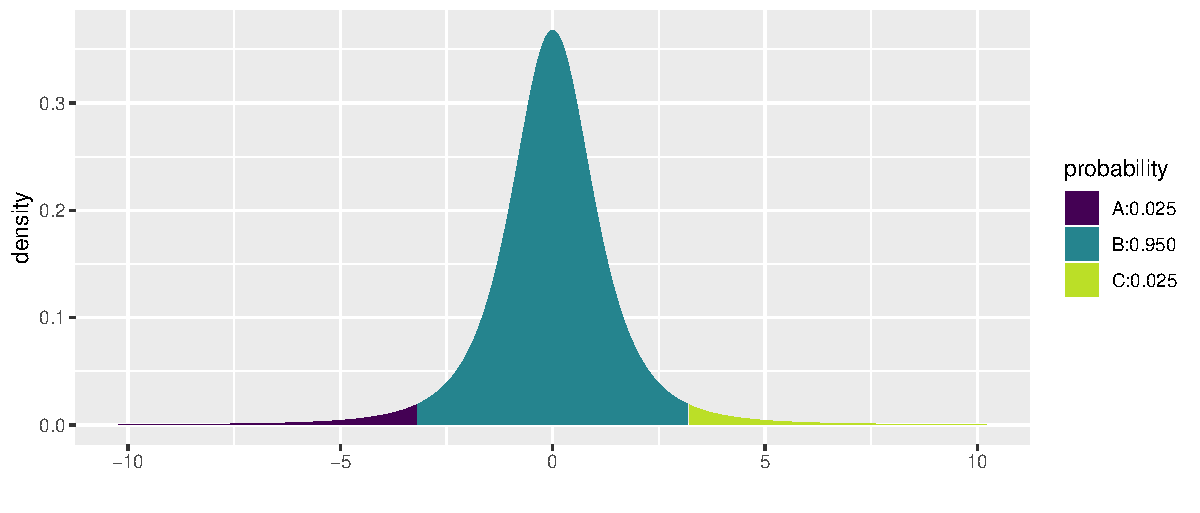
\includegraphics[width=1\linewidth]{figure/unnamed-chunk-30-1} 

}


\begin{verbatim}
## [1] -3.182446  3.182446
\end{verbatim}

\end{knitrout}

\end{frame}




\begin{frame}{Summary of $t$ distribution}
\mylist{Its harder to reject the null when using the $t$ distribution; \pause Confidence intervals are also wider; \pause This is due to our uncertainty about the estimated variance ;\pause Larger samples lead to more accurate estimates of $\sigma$; \pause This is reflected in the fact that there is a different $t$ distribution for each sample size  ; \pause As $n \rightarrow \infty$, sample standard deviation $s$ gets closer to $\sigma$; \pause As degrees of freedom increase, $t$ distribution gets closer to Normal distribution}
\end{frame}


\section{Examples}


\begin{frame}{Application: How fast is your reaction time?}
\small\url{https://faculty.washington.edu/chudler/java/redgreen.html} 

\framedgraphic{JHReactionTimes.png}

\end{frame}


\begin{frame}[fragile]{Application: How fast is your reaction time?}
\begin{knitrout}\scriptsize
\definecolor{shadecolor}{rgb}{0.969, 0.969, 0.969}\color{fgcolor}
\begin{alltt}
\hlstd{reaction.times} \hlkwb{<-} \hlkwd{c}\hlstd{(}\hlnum{325}\hlstd{,}\hlnum{327}\hlstd{,}\hlnum{357}\hlstd{,}\hlnum{299}\hlstd{,}\hlnum{378}\hlstd{)}\hlopt{/}\hlnum{1000}
\hlkwd{summary}\hlstd{(reaction.times)}
\end{alltt}
\begin{verbatim}
##    Min. 1st Qu.  Median    Mean 3rd Qu.    Max. 
##  0.2990  0.3250  0.3270  0.3372  0.3570  0.3780
\end{verbatim}
\begin{alltt}
\hlkwd{round}\hlstd{(}\hlkwd{sd}\hlstd{(reaction.times),}\hlnum{3}\hlstd{)}
\end{alltt}
\begin{verbatim}
## [1] 0.031
\end{verbatim}
\begin{alltt}
\hlkwd{length}\hlstd{(reaction.times)}
\end{alltt}
\begin{verbatim}
## [1] 5
\end{verbatim}

\end{knitrout}

\end{frame}


\begin{frame}[fragile]{5 ways of calculating a confidence interval}

We are interested in calculating a 95\% confidence interval for the mean reaction time based on the sample of 5 reaction times. \\ \ \\
\pause
Five ways of doing this:
\begin{enumerate}
	\setlength\itemsep{1em}
	\item By hand (using the $\pm$ formula and \texttt{R} as a calculator)
	\item Using the quantile function for the $t$ distribution \texttt{stats::qt}
	\item Fitting an intercept-only regression model ($y = \beta_0 + \varepsilon$)
	\item Using a canned function (\texttt{mosaic::t.test}, \texttt{stats::t.test})
	\item Bootstrap
\end{enumerate}

\end{frame}

\begin{frame}[fragile]{1. By hand using the $\pm$ formula}
\begin{knitrout}\scriptsize
\definecolor{shadecolor}{rgb}{0.969, 0.969, 0.969}\color{fgcolor}
\begin{alltt}
\hlstd{n} \hlkwb{<-} \hlkwd{length}\hlstd{(reaction.times)}
\hlstd{SEM} \hlkwb{<-} \hlkwd{sd}\hlstd{(reaction.times)}\hlopt{/}\hlkwd{sqrt}\hlstd{(n)}
\end{alltt}
\begin{verbatim}
## [1] 0.01372734
\end{verbatim}
\begin{alltt}
\hlstd{ybar} \hlkwb{<-} \hlkwd{mean}\hlstd{(reaction.times)}
\end{alltt}
\begin{verbatim}
## [1] 0.3372
\end{verbatim}
\begin{alltt}
\hlstd{multiple.for.95pct} \hlkwb{<-} \hlstd{stats}\hlopt{::}\hlkwd{qt}\hlstd{(}\hlkwc{p} \hlstd{=} \hlkwd{c}\hlstd{(}\hlnum{0.025}\hlstd{,} \hlnum{0.975}\hlstd{),} \hlkwc{df} \hlstd{= n}\hlopt{-}\hlnum{1}\hlstd{)}
\end{alltt}
\begin{verbatim}
## [1] -2.776445  2.776445
\end{verbatim}
\begin{alltt}
\hlstd{by_hand_CI} \hlkwb{<-} \hlstd{ybar} \hlopt{+} \hlstd{multiple.for.95pct} \hlopt{*} \hlstd{SEM}
\end{alltt}
\begin{verbatim}
## [1] 0.29909 0.37531
\end{verbatim}

\end{knitrout}
\end{frame}

\begin{frame}[fragile]{2. Using \texttt{stats::qt}}
\textit{Note: \texttt{R} only provides the standard $t$ distribution. In order to get a scaled version we must define our own function.}

\vspace*{0.2in}

\begin{knitrout}\scriptsize
\definecolor{shadecolor}{rgb}{0.969, 0.969, 0.969}\color{fgcolor}
\begin{alltt}
\hlstd{n} \hlkwb{<-} \hlkwd{length}\hlstd{(reaction.times)}
\hlstd{SEM} \hlkwb{<-} \hlkwd{sd}\hlstd{(reaction.times)}\hlopt{/}\hlkwd{sqrt}\hlstd{(n)}
\hlstd{ybar} \hlkwb{<-} \hlkwd{mean}\hlstd{(reaction.times)}

\hlcom{# scaled version of the standard t distribution}
\hlstd{qt_ls} \hlkwb{<-} \hlkwa{function}\hlstd{(}\hlkwc{p}\hlstd{,} \hlkwc{df}\hlstd{,} \hlkwc{mean}\hlstd{,} \hlkwc{sd}\hlstd{)} \hlkwd{qt}\hlstd{(}\hlkwc{p} \hlstd{= p,} \hlkwc{df} \hlstd{= df)} \hlopt{*} \hlstd{sd} \hlopt{+} \hlstd{mean}

\hlkwd{qt_ls}\hlstd{(}\hlkwc{p} \hlstd{=} \hlkwd{c}\hlstd{(}\hlnum{0.025}\hlstd{,} \hlnum{0.975}\hlstd{),} \hlkwc{df} \hlstd{= n} \hlopt{-} \hlnum{1}\hlstd{,} \hlkwc{mean} \hlstd{= ybar,} \hlkwc{sd} \hlstd{= SEM)}
\end{alltt}
\begin{verbatim}
## [1] 0.2990868 0.3753132
\end{verbatim}

\end{knitrout}
\end{frame}


\begin{frame}[fragile]{3. Fitting an intercept-only regression model}
\begin{knitrout}\scriptsize
\definecolor{shadecolor}{rgb}{0.969, 0.969, 0.969}\color{fgcolor}
\begin{alltt}
\hlstd{fit} \hlkwb{<-} \hlstd{stats}\hlopt{::}\hlkwd{lm}\hlstd{(reaction.times} \hlopt{~} \hlnum{1}\hlstd{)}
\hlkwd{summary}\hlstd{(fit)}
\end{alltt}
\begin{verbatim}
## 
## Call:
## stats::lm(formula = reaction.times ~ 1)
## 
## Residuals:
##       1       2       3       4       5 
## -0.0122 -0.0102  0.0198 -0.0382  0.0408 
## 
## Coefficients:
##             Estimate Std. Error t value Pr(>|t|)    
## (Intercept)  0.33720    0.01373   24.56 1.63e-05 ***
## ---
## Signif. codes:  0 '***' 0.001 '**' 0.01 '*' 0.05 '.' 0.1 ' ' 1
## 
## Residual standard error: 0.0307 on 4 degrees of freedom
\end{verbatim}
\begin{alltt}
\hlstd{stats}\hlopt{::}\hlkwd{confint}\hlstd{(fit)}
\end{alltt}
\begin{verbatim}
##                 2.5 %    97.5 %
## (Intercept) 0.2990868 0.3753132
\end{verbatim}

\end{knitrout}
\end{frame}


\begin{frame}[fragile]{3. Fitting an intercept-only regression model}
In the regression output:
\begin{itemize}
	\setlength\itemsep{1em}
	\item \texttt{Estimate}: the mean reaction time (an estimate of the intercept $\beta_0$)
	\item \texttt{t value}: the test statistic 
	\item \texttt{Std. Error}: the standard error of the mean (SEM)
	\item \texttt{Pr(>|t|)}: is the $p$-value
\end{itemize} 


\end{frame}


\begin{frame}[fragile]{3. Fitting an intercept-only regression model}



\small
These are based on the (useless) null hypothesis $H_0: \mu_0 = 0$ \\ \ \\

\begin{itemize}
	\item \texttt{t value} = $\frac{\bar{y} - \mu_0}{s / \sqrt{n}}$ = $\frac{0.33720 - 0}{0.01373}$ = 24.56
	\item \texttt{Pr(>|t|)} \\ \ \\
	= $P(\textrm{t value} > t_{(n-1)}) + P(-\textrm{t value} < t_{(n-1)})$ \\ \ \\
	 = \small{\texttt{pt(q = 24.56, df = n-1, lower.tail = FALSE)} +  \texttt{pt(q = -24.56, df = n-1)}} \\ \ \\
	  = \ensuremath{8.1549827\times 10^{-6}} + \ensuremath{8.1549827\times 10^{-6}} = \ensuremath{1.6309965\times 10^{-5}}
\end{itemize}


\end{frame}



\begin{frame}[fragile]{4. Canned function}

\begin{knitrout}\scriptsize
\definecolor{shadecolor}{rgb}{0.969, 0.969, 0.969}\color{fgcolor}
\begin{alltt}
\hlstd{stats}\hlopt{::}\hlkwd{t.test}\hlstd{(reaction.times)}
\end{alltt}
\begin{verbatim}
## 
## 	One Sample t-test
## 
## data:  reaction.times
## t = 20, df = 4, p-value = 2e-05
## alternative hypothesis: true mean is not equal to 0
## 95 percent confidence interval:
##  0.299 0.375
## sample estimates:
## mean of x 
##     0.337
\end{verbatim}

\end{knitrout}

\end{frame}



\begin{frame}[fragile]{5. Bootstrap}

\begin{knitrout}\scriptsize
\definecolor{shadecolor}{rgb}{0.969, 0.969, 0.969}\color{fgcolor}
\begin{alltt}
\hlstd{df_react} \hlkwb{<-} \hlkwd{data.frame}\hlstd{(reaction.times)} \hlcom{# need data.frame to bootstrap}
\hlstd{s_dist} \hlkwb{<-} \hlkwd{do}\hlstd{(}\hlnum{10000}\hlstd{)} \hlopt{*} \hlkwd{mean}\hlstd{(} \hlopt{~} \hlstd{reaction.times,}
                \hlkwc{data} \hlstd{=} \hlkwd{resample}\hlstd{(df_react))}
\hlstd{CI_95} \hlkwb{<-} \hlkwd{quantile}\hlstd{(}\hlopt{~} \hlstd{mean,} \hlkwc{data} \hlstd{= s_dist,} \hlkwc{probs} \hlstd{=} \hlkwd{c}\hlstd{(}\hlnum{0.025}\hlstd{,} \hlnum{0.975}\hlstd{))}
\end{alltt}
\begin{verbatim}
##  2.5% 97.5% 
## 0.315 0.362
\end{verbatim}


{\centering 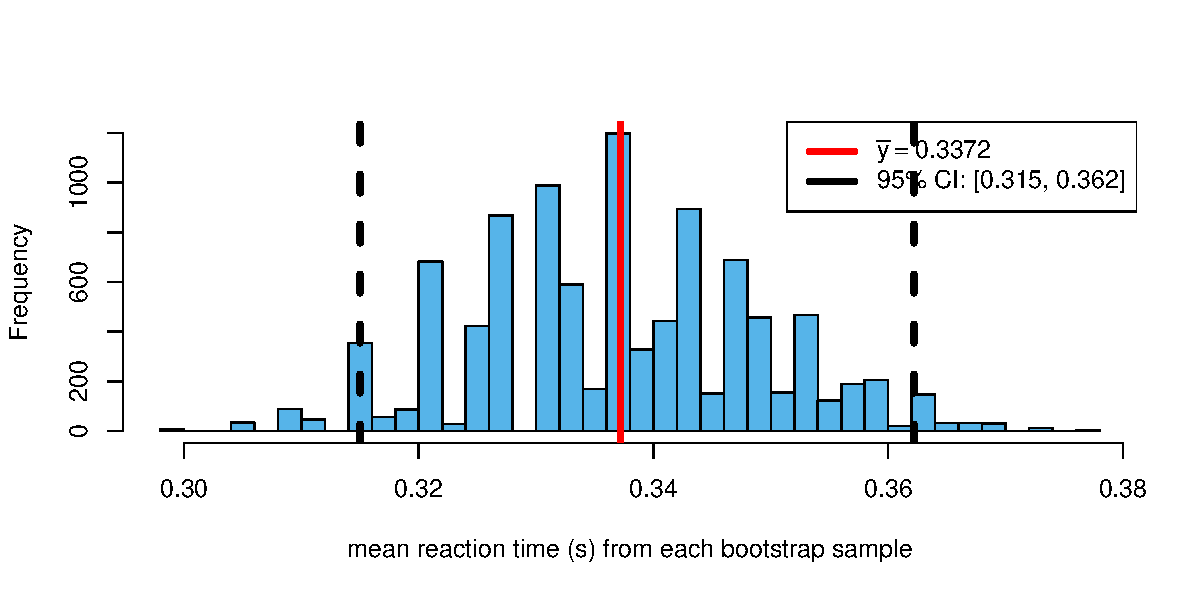
\includegraphics[width=1\linewidth]{figure/unnamed-chunk-37-1} 

}



\end{knitrout}

\end{frame}


\begin{frame}{Summary}
\begin{itemize}
	\setlength\itemsep{1em}
	\item We use $t$ procedures instead of $Z$ when we have very small samples ($n \leq 30$)
	\item This is because our estimate of $\sigma$ is probably not accurate with such a small sample
	\item We account for this extra uncertainty by widening the interval $\to$ larger multiplicative factor ($t_{(n-1)}$ > $z^\star$) \pause 
	\item Reality check: It is unlikely you will have such a small sample unless you're working with rats
	\item In practice you don't need to worry about $t$ vs. $Z$. The software does it for you.
	\item However, you should still understand where the numbers are coming from and how it is being calculated. Computers aren't intelligent, they're just well trained. 
\end{itemize}
\end{frame}


\end{document}






